%Autores: Prof. Phyllipe Lima
%         Daylon Ramos da Silva
%Contato: phyllipe@inatel.br / phyllipe_slf@yahoo.com.br
%         biblioteca.pesquisa@inatel.br
%Modelo para escrita de artigos científicos para o TCC dos cursos Graduação do INATEL - Instituto Nacional de Telecomunicações. 
%Este template LaTeX é uma adaptação do modelo doc desenvolvido pelos professores Carlos Ynoguti e Dayan Guimarães

%Se você é novo no latex, um bom lugar para começar é
%https://pt.overleaf.com/learn
\documentclass[10pt,twocolumn]{article} 
%Use esse arquivo para incluir novos pacotes

\usepackage[%usado para determinar medidas
top=1.78cm,
bottom=1.78cm,
left=1.65cm,
right=1.65cm,
headsep=0cm,
%showframe
]{geometry}
%\usepackage[justification=centering]{caption}
\usepackage{inatel}%carregar algumas estilizacoes do inatel
\usepackage{times}
\usepackage{xcolor}
% initialize math tools
\usepackage{bm}
\usepackage{amsmath}
% sinc
\DeclareMathOperator{\sinc}{sinc}
\usepackage{cancel}
\usepackage{amssymb}
\usepackage{mathtools}
\usepackage{empheq}
\usepackage{arydshln}
\usepackage{steinmetz}
% define equal
\newcommand\eqdef{\mathrel{\overset{\makebox[0pt]{\mbox{\normalfont\tiny\sffamily def}}}{=}}}
% multirow in Tables
\usepackage{multirow}
% change title size
\usepackage{titlesec}
\titleformat*{\section}{\centering\huge}
% MATLAB Code Block
\usepackage[framed,numbered,autolinebreaks,useliterate]{mcode}
\usepackage{enumitem}%redefinir espacos itemize
\usepackage{graphicx}
\usepackage{url,hyperref}
\usepackage[utf8]{inputenc}
\usepackage{float}%mais controle para manipular figuras
\usepackage{caption}%manipular legenda da figura e tabela
\usepackage{mathtools}%equacoes
\usepackage[hang,flushmargin]{footmisc} 
\usepackage{xcolor}
\usepackage{wrapfig} %usado para envolver figura com texto
%\usepackage[portuguese]{babel}
\usepackage{fancyhdr}%criacao do cabecalho
\usepackage{etoolbox}
\usepackage{adjustbox}%mais controle para ajustar tamanho da tabela
\usepackage{comment}%ambiente para comentario
\usepackage{relsize} %usado por comandos \mathlarger
%\usepackage{mathptmx}

%Referencia bibliografica
\usepackage[
    style=numeric,
    sorting=none,
    maxbibnames=10]{biblatex}
\addbibresource{referencia.bib}

% better underlines
\usepackage{soul}

%Idioma. Use "english" para trabalhos em inglês
\usepackage[brazil]{babel}

\newcommand{\volume}{{\ooalign{\hfil$V$\hfil\cr\kern0.08em--\hfil\cr}}}
%Ajustes na legenda da figura. Incluindo espacamento apos a legenda
\captionsetup[figure]{labelformat={default},labelsep=period,font=footnotesize, name=\footnotesize{Fig.},justification=raggedright,singlelinecheck=false,belowskip=-0.9\normalbaselineskip}
%\pagenumbering{gobble}

%Ajustes na legenda da tabela. 
\captionsetup[table]{labelformat={default},labelsep=newline,font={sc,footnotesize},justification=centering,singlelinecheck=false}

\renewcommand{\headrulewidth}{0pt}


\begin{document}

\title{\Huge \bf MECH3610 Cheat Sheet}
\author{\large Currently maintained by: D.S.}

\maketitle

\section{Week 1}
\textbf{\large Terminologies}
\begin{table}[h]
\begin{tabular}{|l|l|l|}
\hline
\textbf{Jargon} & \textbf{Symbol}    & \textbf{Unit} \\ \hline
Heat            & $Q$                & $[J]$         \\ \hline
Heat rate       & $\dot{Q}=Q/t$      & $[W]$         \\ \hline
Heat flux       & $q''=\dot{Q}/A$ & $[W/m^2]$      \\ \hline
\end{tabular}
\end{table}

\textbf{\large Mode of Heat Transfer}
\begin{itemize}
    \item \underline{\textbf{Conduction:}} Energy transfer from \color{red} more energetic \color{black} particles to \color{red} less energetic \color{black} particles of a substance; requires medium.
    
    \textbf{Fourier's law of heat conduction:}
    \begin{align*}
       \dot{Q} &= -kA\frac{T_2-T_1}{\Delta x} = -kA \frac{\Delta T}{\Delta x}, \; \; [W] \\
        q'' &= -k\frac{T_2-T_1}{\Delta x} = k \frac{T_1-T_2}{\Delta x}, \; \; [W/m^2]\\
        \text{where } k &= \text{thermal conductivity, [$W/m\cdot K$]}
    \end{align*}
    \begin{figure}[h]
        \centering
        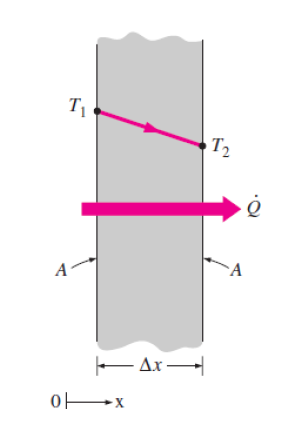
\includegraphics[width=0.5\linewidth]{images/conduction.png}
    \end{figure}
    \item \underline{\textbf{Convection:}} Energy transfer between a solid surface and an adjacent liquid/gas in motion; combined effects of \color{red} conduction \color{black} and \color{red} fluid motion \color{black}; requires medium.
    
    \textbf{Newton's Law of Cooling:}
    \begin{align*}
        \dot{Q} &= h A_s (T_s - T_{\infty}), \; \; [W] \\
        q'' &= h (T_s - T_{\infty}), \; \; [W/m^2] \\
        \text{where } T_s &= \text{temp. of the surface,} \\
        T_{\infty} &= \text{temp. of fluid far from surface,} \\
        A_s &= \text{surface area,} \\
        h &= \text{convection coefficient, [$W/m^2\cdot K$]}
    \end{align*}
    \item \underline{\textbf{Radiation:}} Energy that is emitted by matter and is transported as \color{red} electromagnetic waves / photons \color{black}; does not require medium.
    \begin{figure}[h]
        \centering
        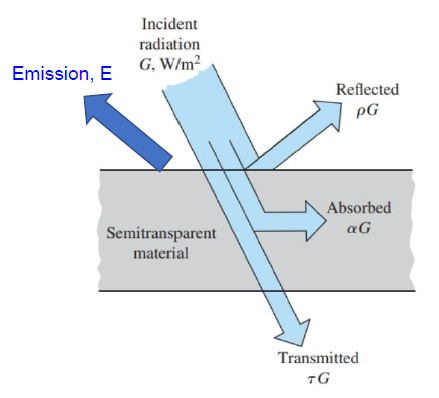
\includegraphics[width=0.75\linewidth]{images/radiation.png}
    \end{figure}
    \begin{align*}
        \rho + \alpha + \tau &= 1, \; \; \text{(for any medium)} \\
        \rho + \alpha &= 1, \; \; \text{(for opaque medium)} \\
        \text{where } \rho &= \text{fraction of G reflected,} \\
        \alpha &= \text{fraction of G absorbed,} \\
        \tau &= \text{fraction of G transmitted through the medium.}
    \end{align*}
    \textbf{Kirchoff's Law of Thermal Radiation:}
    \begin{equation*}
        \alpha = \epsilon \; \; \text{(for most cases)}
    \end{equation*}
    \textbf{Emissive Power E:} 
    \begin{align*}
        E &= \sigma \epsilon T_{s}^{4}, \; \; [W/m^2] \\
        \dot{Q}_E &= \sigma A_s \epsilon T_s^4, \; \; [W]\\
        \text{where } \sigma &= 5.67\times 10^{-8} \; W/m^2 K^4 \; \; \text{(Stefan-Boltzmann constant)} \\
        \epsilon &= \text{Emissivity} 
    \end{align*}
    \textbf{Irradiation G:}
    \begin{align*}
        G_{total} &= (\alpha + \beta + \tau) \sigma T_{surr}^4 \\
        &= \sigma T_{surr}^4 \\
        G_{absorbed} &= \alpha \sigma T_{surr}^4 \\
        &= \epsilon \sigma T_{surr}^4
    \end{align*}
    \textbf{Special case:} surface exposed to large surroundings of uniform temperature $T_{surr}$
    \begin{figure}[h]
        \centering
        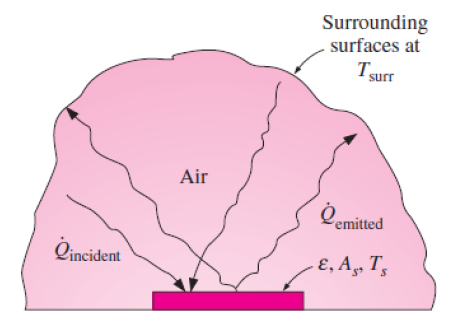
\includegraphics[width=0.7\linewidth]{images/radiation_special_case.png}
    \end{figure}
    \begin{align*}
        \dot{Q} &= E- G_{absorbed} \\
        &= A_s \left(\underbrace{\epsilon \sigma T_s^4}_{E} - \underbrace{\alpha \sigma T_{surr}^4}_{\alpha G}\right) \\
        &= \sigma A_s \epsilon (T_s^4 - T_{surr}^4)
    \end{align*}
    Alternatively,
    \begin{align*}
        \dot{Q} &= h_r A_s (T_s - T_{surr} ) \\
        \text{where } h_r &= \text{radiation heat transfer coefficient, W/$m^2$K}\\ 
        &=\epsilon \sigma (T_s + T_{surr})(T_s^2+T_{surr}^2)
    \end{align*}
    \item \textbf{\color{red}Overall\color{black}} heat flux for radiation:
    \begin{equation*}
        \dot{Q} = E + (\rho - \alpha - \tau) \cdot G
    \end{equation*}
    \item \textbf{\color{red}Net\color{black}} heat flux for radiation:
    \begin{align*}
        \dot{Q} &= \text{total leaving surface} - \text{total approaching surface} \\
        \dot{Q} &= E + (\rho+\tau ) G - G
    \end{align*}
\end{itemize}

\large\textbf{Heat Generation}
\begin{itemize}
    \item Unit of heat generation $\dot{g}$: [W/$m^3$]
    \item Rate of heat generation: $\dot{Q}=\dot{g}V$ [W]
    \item Surface Temperature: $T_s = T_{\infty}+\frac{\dot{g}V}{h A_s}$
    \item For \underline{\textbf{large plane wall}} of thickness $2L$:
    \begin{align*}
        A_s&=2A_{wall} \\
        V &=2LA_{wall} \\
        T_{\text{s,plane wall}} &= T_{\infty}+\frac{\dot{g}L}{h}
    \end{align*}
    \item For \underline{\textbf{solid cylinder}} of radius $r_o$:
    \begin{align*}
        A_s &= 2\pi r_o L \\
        V &=\pi r_o^2 L \\
        T_{\text{s,cylinder}} &= T_{\infty} + \frac{\dot{g}r_o}{2h}
    \end{align*}
    \item For \underline{\textbf{sphere}} of radius $r_o$:
    \begin{align*}
        A_s &= 4\pi r_o^2 \\
        V &= \frac{4}{3} \pi r_o^3 \\
        T_{\text{s,sphere}} &= T_{\infty} + \frac{\dot{g}r_o}{3h} 
    \end{align*}
\end{itemize}

\large\textbf{Max Temperature}
\begin{figure}[h]
    \centering
    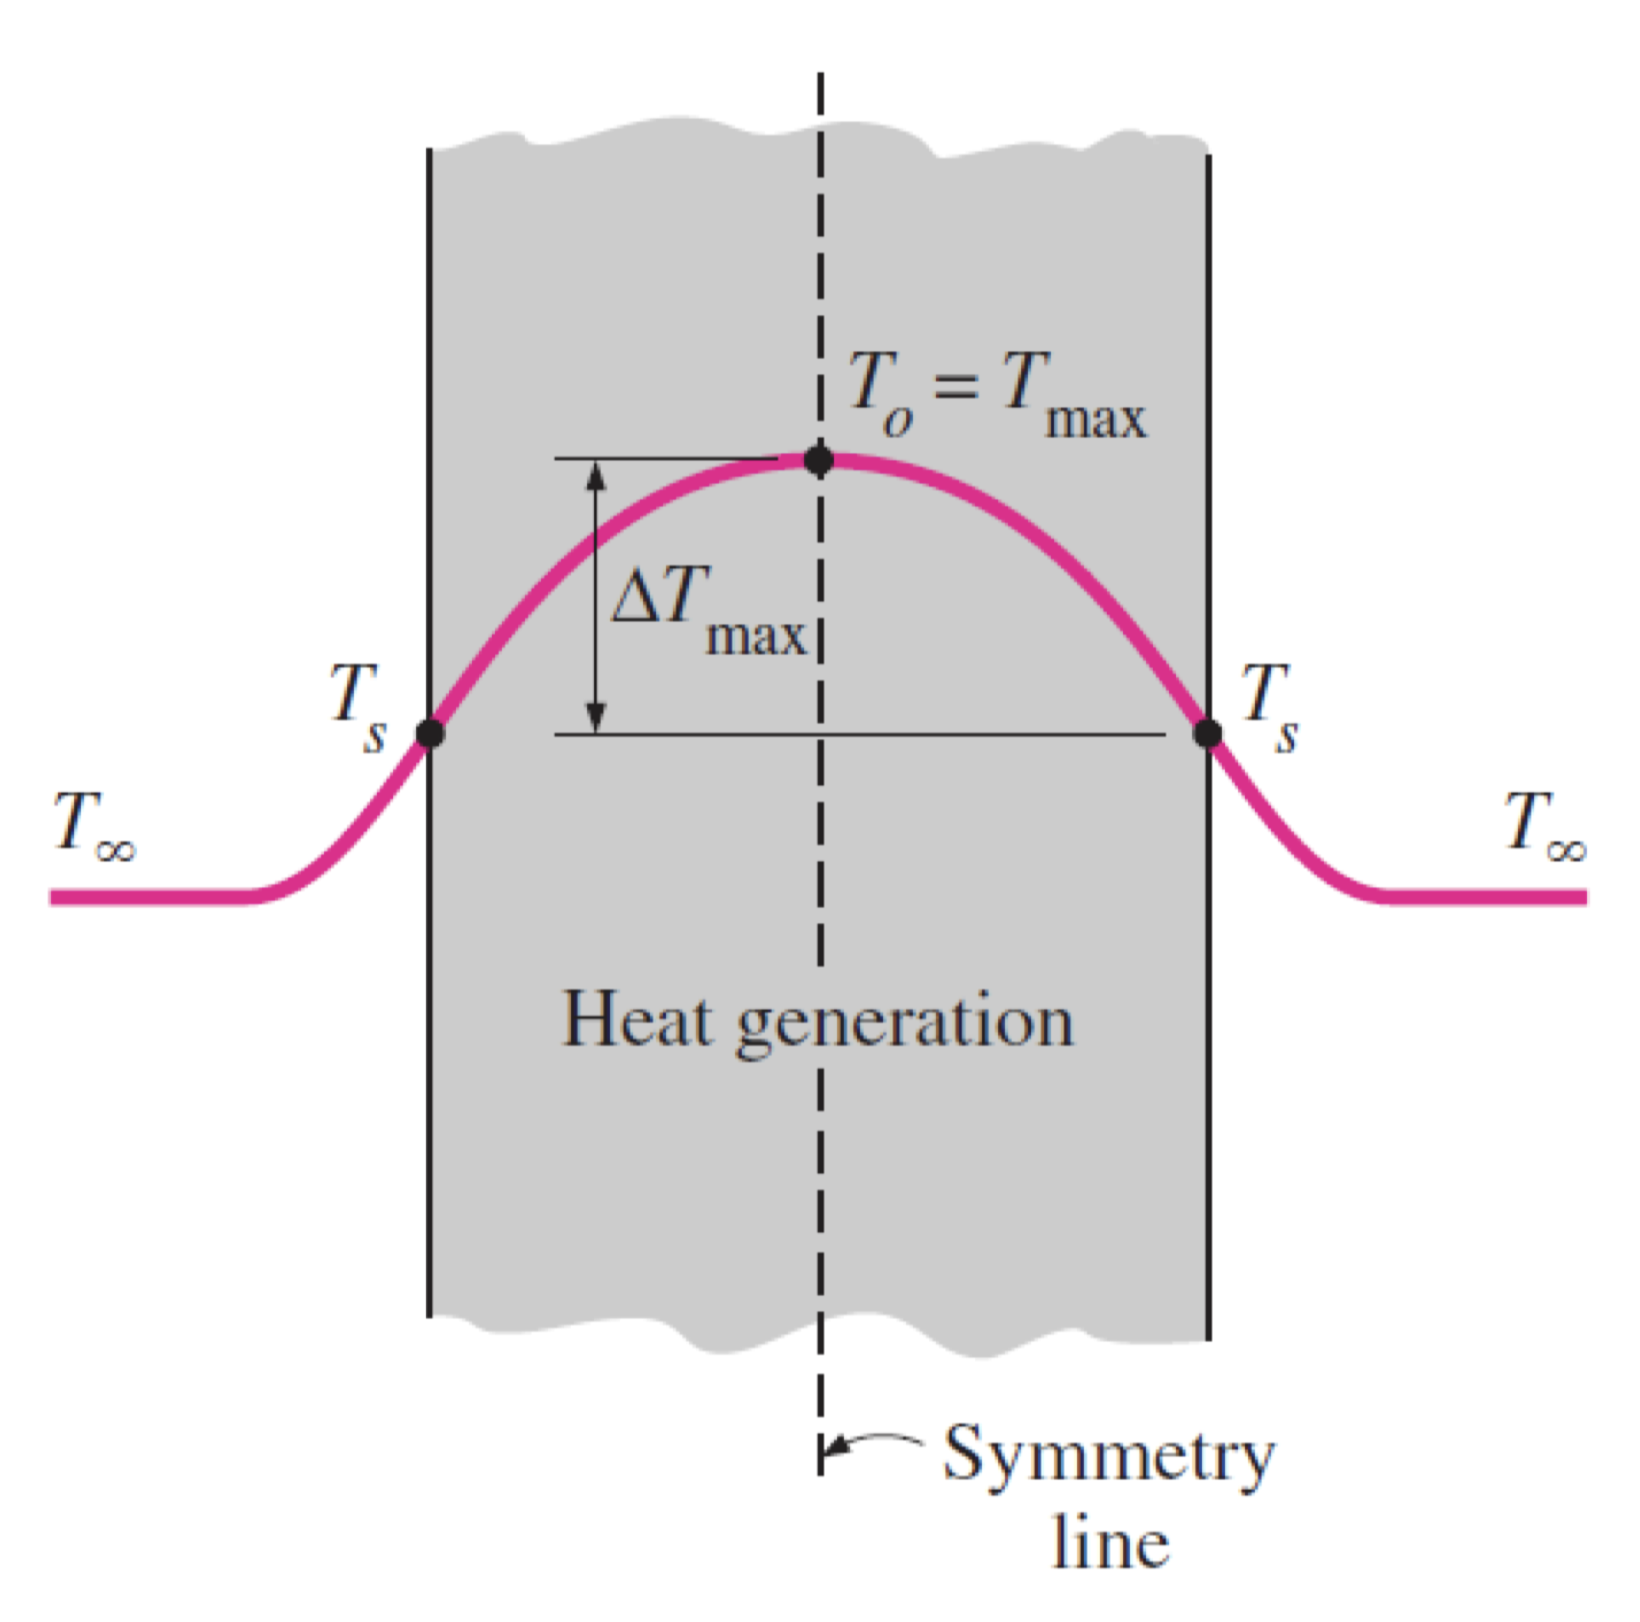
\includegraphics[width=0.75\linewidth]{images/heat_generation_max_temp.png}
\end{figure}

\begin{align*}
    \Delta T_{\text{max,cylinder}}&= T_o - T_s = \frac{\dot{g}r_o^2}{4k} \\
    \Delta T_{\text{max,plane wall}} &= \frac{\dot{g}L^2}{2k} \\
    \Delta T_{\text{max,sphere}} &= \frac{\dot{g}r_o^2}{6k}
\end{align*}

\large\textbf{Heat Equations}
\begin{enumerate}
    \item Heat conduction through \color{red} large plane wall: \color{black}
    \begin{equation*}
        \frac{\partial^2 T}{\partial x^2} + \frac{\dot{e}_g}{k} = \frac{1}{\alpha} \frac{\partial T}{\partial t}
    \end{equation*}
    \item Heat conduction in \color{red} long cylinder: \color{black}
    \begin{equation*}
        \frac{1}{r} \frac{\partial}{\partial r}\left(r \frac{\partial T}{\partial r}\right) + \frac{\dot{e}_g}{k} = \frac{1}{\alpha} \frac{\partial T}{\partial t}
    \end{equation*}
    \item Heat conduction in \color{red} sphere: \color{black}
    \begin{equation*}
        \frac{1}{r^2} \frac{\partial}{\partial r} \left( r^2 \frac{\partial T}{\partial r}\right) + \frac{\dot{e}_g}{k} = \frac{1}{\alpha} \frac{\partial T}{\partial t}
    \end{equation*}
\end{enumerate}

\large\textbf{Thermal Resistance}
\begin{itemize}
    \item Definition:
    \begin{align*}
        R &= \frac{\text{driving force}}{\text{transfer rate}} \\
        &= \frac{T_1 - T_2}{\dot{Q}}\;\; \text{ in [K/W]}
    \end{align*}
    \item Overall heat transfer coefficient UA$:=\frac{1}{\sum R_i}$
    \item For \color{red} plane walls: \color{black}
    \begin{align*}
        R_{cond} &= \frac{L}{kA_s} \\
        R_{conv} &= \frac{1}{h A_s} \\
        R_{rad} &= \frac{1}{h_r A_s}
    \end{align*}
    \item Example:
    \begin{itemize}
        \item In series:
        \begin{figure}[H]
            \centering
            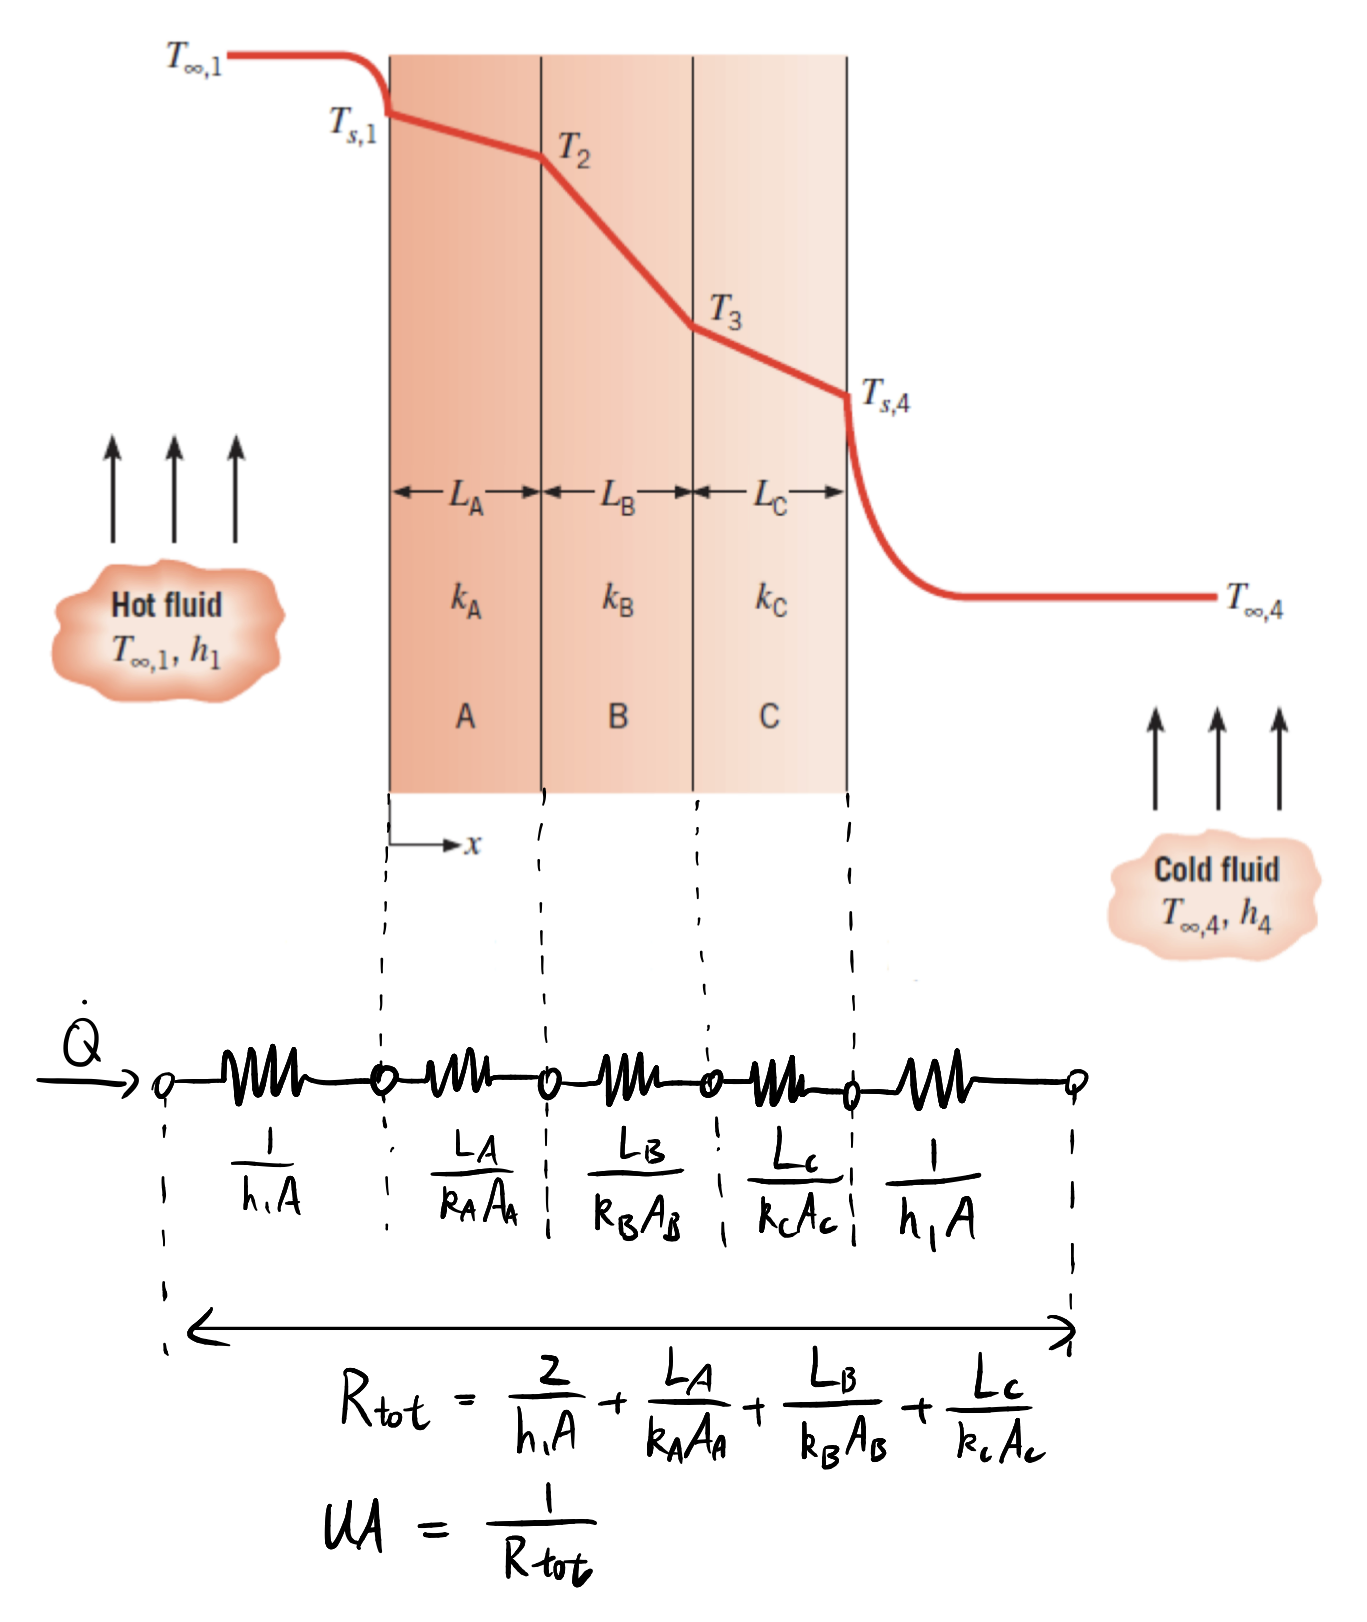
\includegraphics[width=0.85\linewidth]{images/thermal_resistance.png}
        \end{figure}
        \item In parallel:
        \begin{figure}[H]
            \centering
            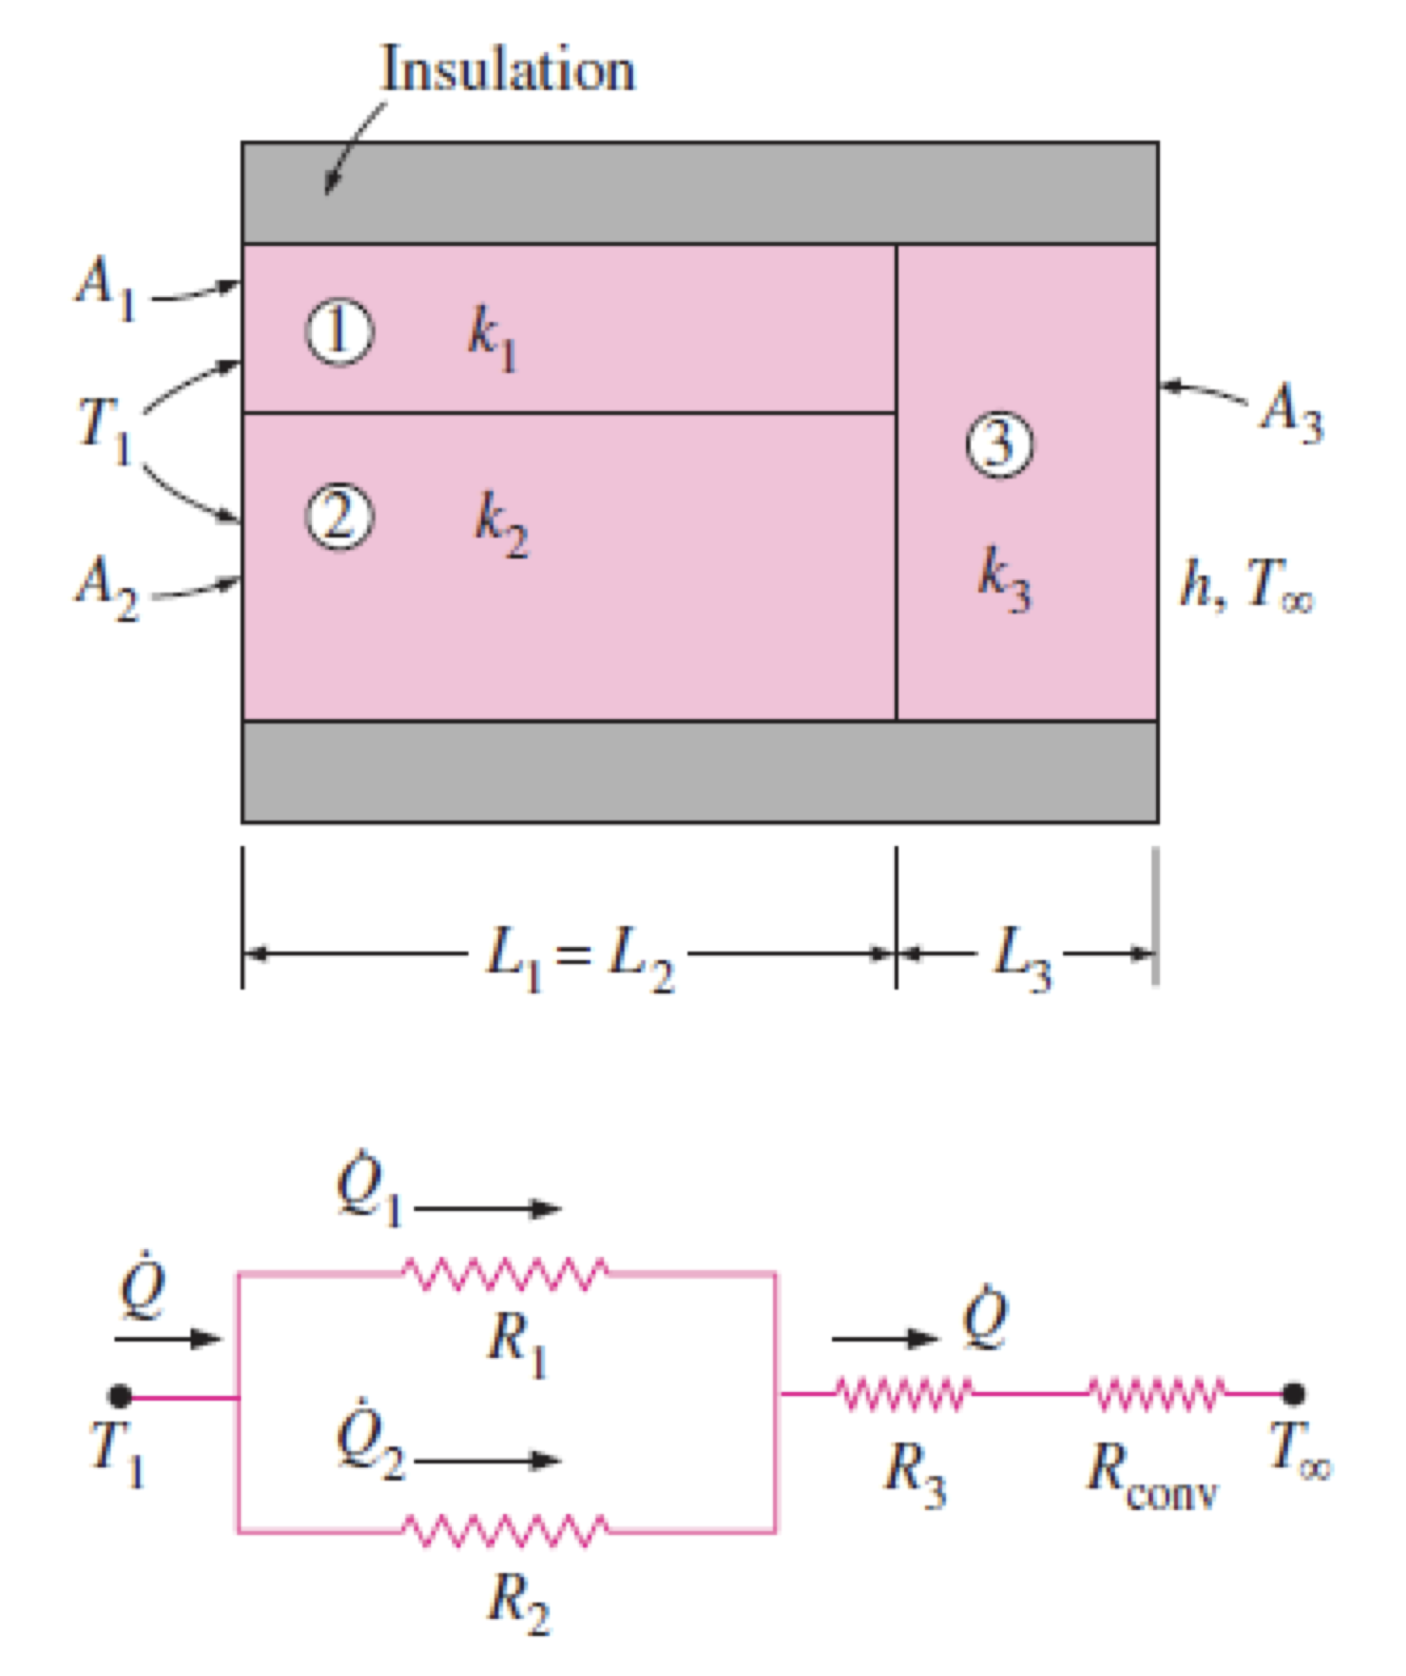
\includegraphics[width=0.7\linewidth]{images/thermal_resistance_parallel.png}
        \end{figure}
        \begin{align*}
            R_{tot} &= \frac{R_1 R_2}{R_1 + R_2} + R_3 + R_{conv} \\
        \end{align*}
        Note that in 1D analyses, we neglect the heat transferred between block 1 and 2.
    \end{itemize}
    \item For \color{red} cylinders: \color{black}
    \begin{figure}[H]
        \centering
        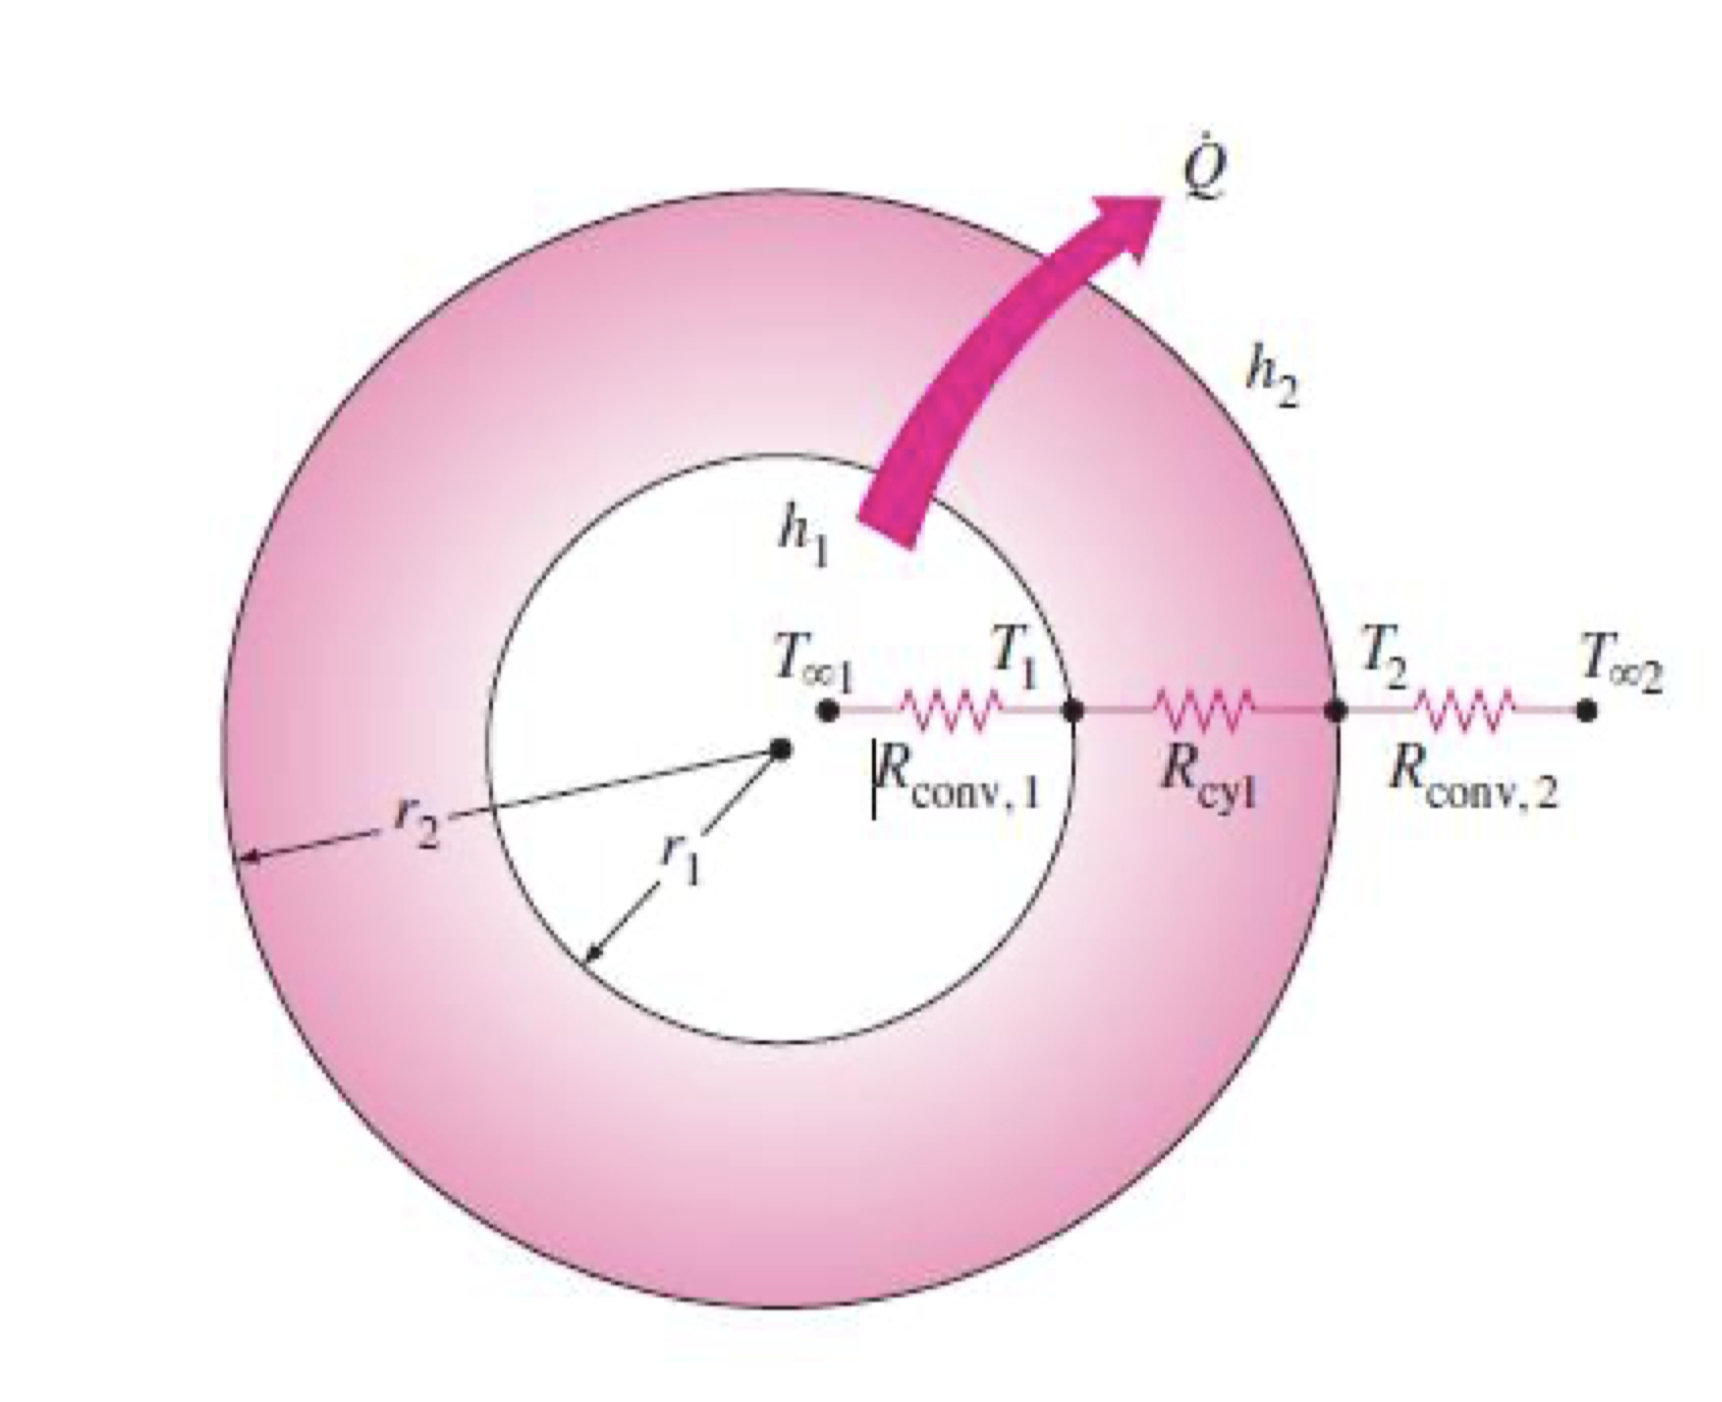
\includegraphics[width=0.9\linewidth]{images/thermal_resistance_cylinder.png}
    \end{figure}
    \begin{align*}
        R_{\text{cyl,cond}} &= \frac{\ln(r_2/r_1)}{2\pi L k} \\
        R_{tot} &= R_{conv,1}+R_{\text{cyl,cond}} + R_{conv,2} \\
        &= \frac{1}{(2\pi r_1 L)h_1} + \frac{\ln(r_2/r_1)}{2\pi L k} + \frac{1}{(2\pi r_2 L)h_2}
    \end{align*}
    \item For \color{red} sphere: \color{black}
    \begin{figure}[H]
        \centering
        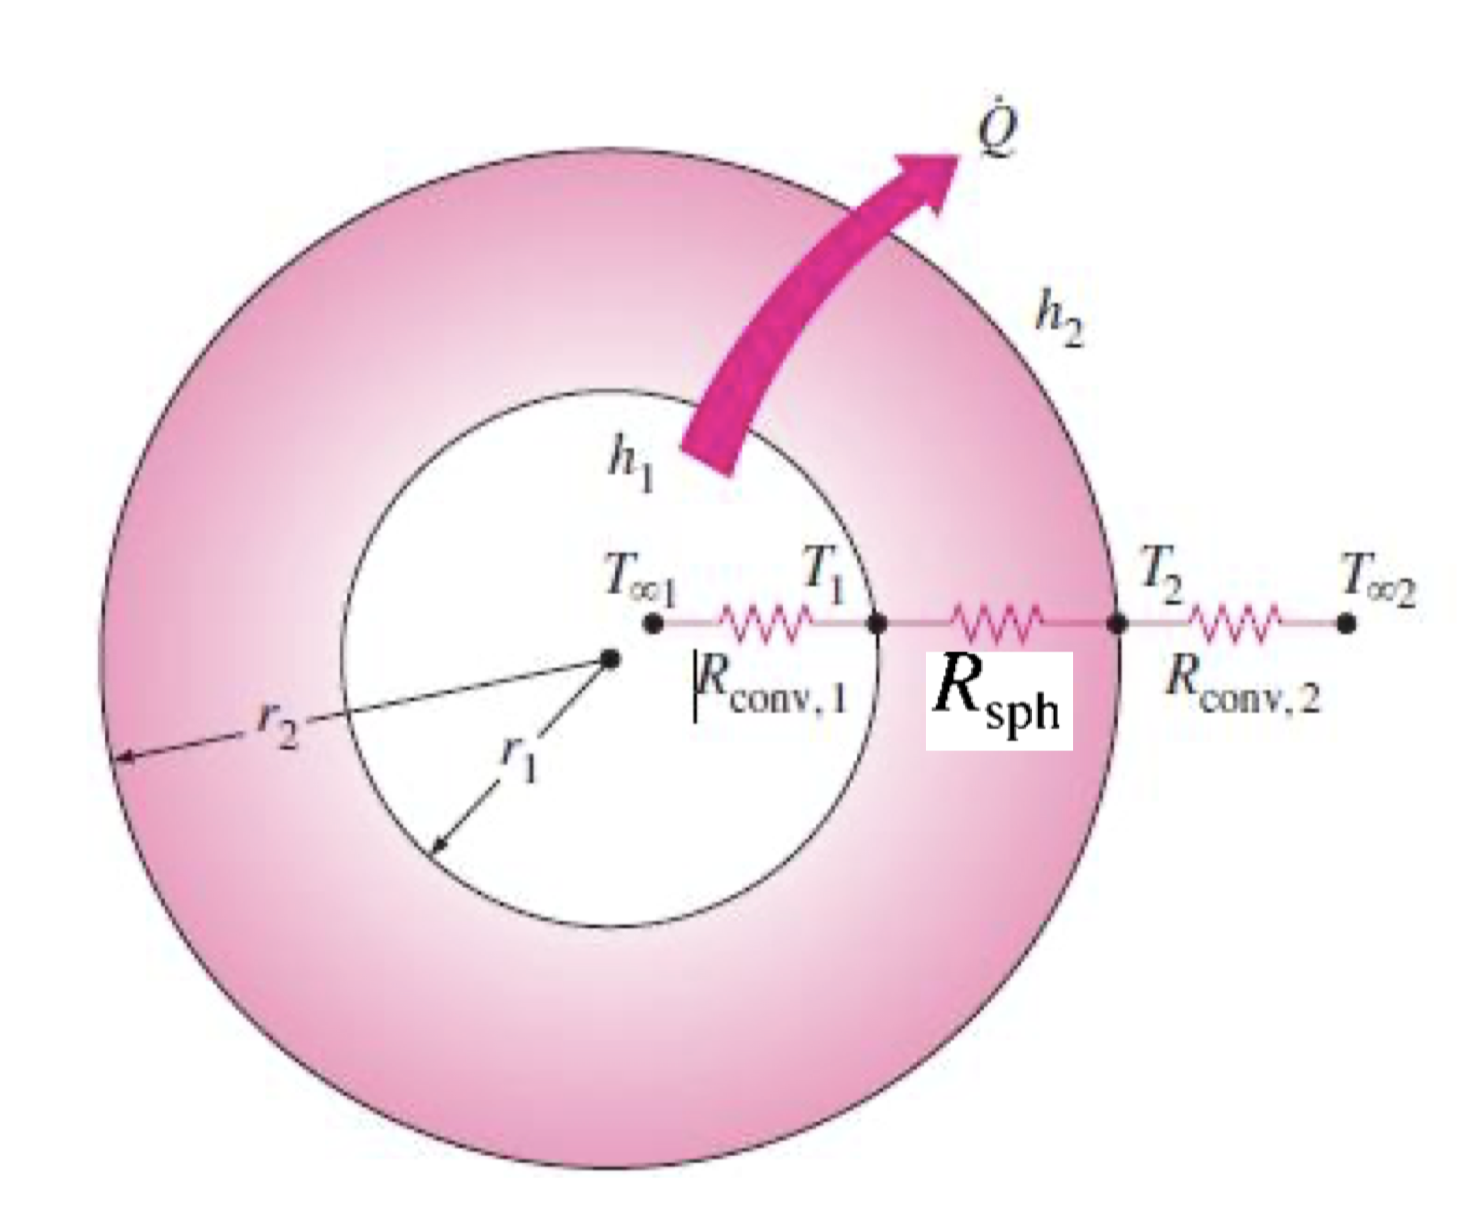
\includegraphics[width=0.9\linewidth]{images/thermal_resistance_sphere.png}
    \end{figure}
    \begin{align*}
        R_{sph} &= \frac{r_2 - r_1}{4\pi r_1 r_2 k} \\
        R_{tot} &= R_{conv,1} + R_{sph} + R_{conv,2} \\
        &= \frac{1}{(4\pi r_1^2)h_1} + \frac{r_2 - r_1}{4\pi r_1 r_2 k} + \frac{1}{(4\pi r_2^2)h_2}
    \end{align*}
    \item For \color{red} radiations: \color{black}
    \begin{align*}
        \dot{Q}_{rad} &= h_r A_s (T_s - T_{surr}) \\
        R_{rad} &= \frac{1}{h_r A}
    \end{align*}
\end{itemize}



\section{Week 2}
\textbf{\large Extended Surfaces: Fins}
\begin{itemize}
    \item Fin Equation:
    \begin{align*}
        \frac{d^2\theta}{dx^2} - m^2 \theta &= 0 \\
        \text{where } \; \theta &= T - T_{\infty} \\
        m^2 &= \frac{hp}{k A_c}
    \end{align*}
    \begin{figure}[H]
        \centering
        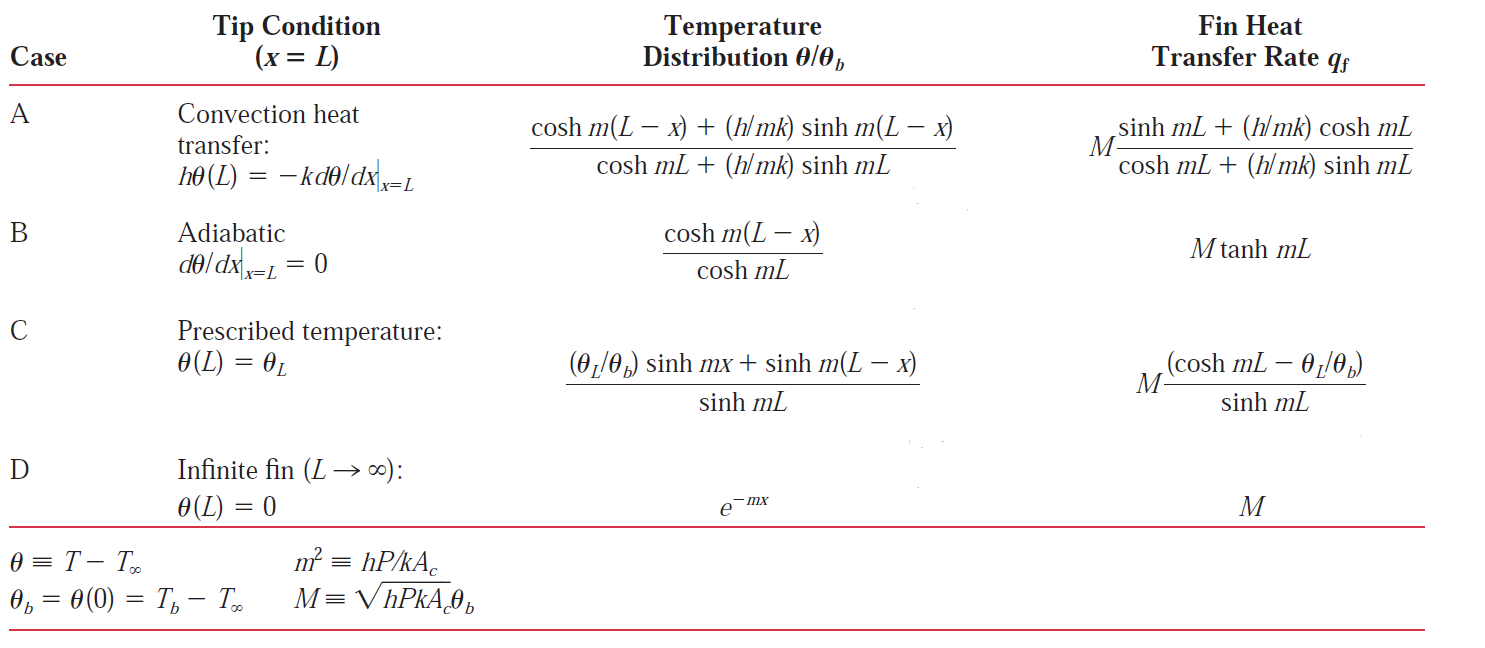
\includegraphics[width=1.0\linewidth]{images/Fin_equations.png}
        \caption{Note that P is the circumference of the cross-section element, and $A_c$ is the area of the cross-section element.}
    \end{figure}
    \item \textbf{\underline{Fin Efficiency:}} defined as the ratio of \color{red} the actual heat transfer rate from the fin \color{black} over \color{blue} ideal heat transfer rate from the fin if the entire fin were at base temperature. \color{black} 
    \begin{align*}
        \eta_{fin} &= \frac{\dot{Q}_{fin}}{\dot{Q}_{fin,max}} \\
        \dot{Q}_{fin} &= \eta_{fin} \dot{Q}_{fin,max} = \eta_{fin}h A_{fin} (T_b - T_{\infty})
    \end{align*}
    \item Corrected fin length $L_c$:
    \begin{equation*}
        L_c = L + \frac{A_c}{p}
    \end{equation*}
    \begin{figure}[H]
        \centering
        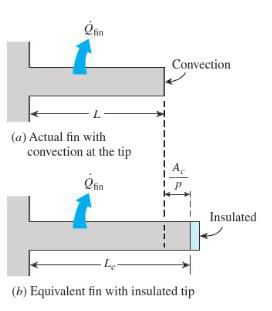
\includegraphics[width=0.6\linewidth]{images/corrected_fin_length.png}
    \end{figure}
    \item List of fin efficiency:
    \begin{figure}[H]
        \centering
        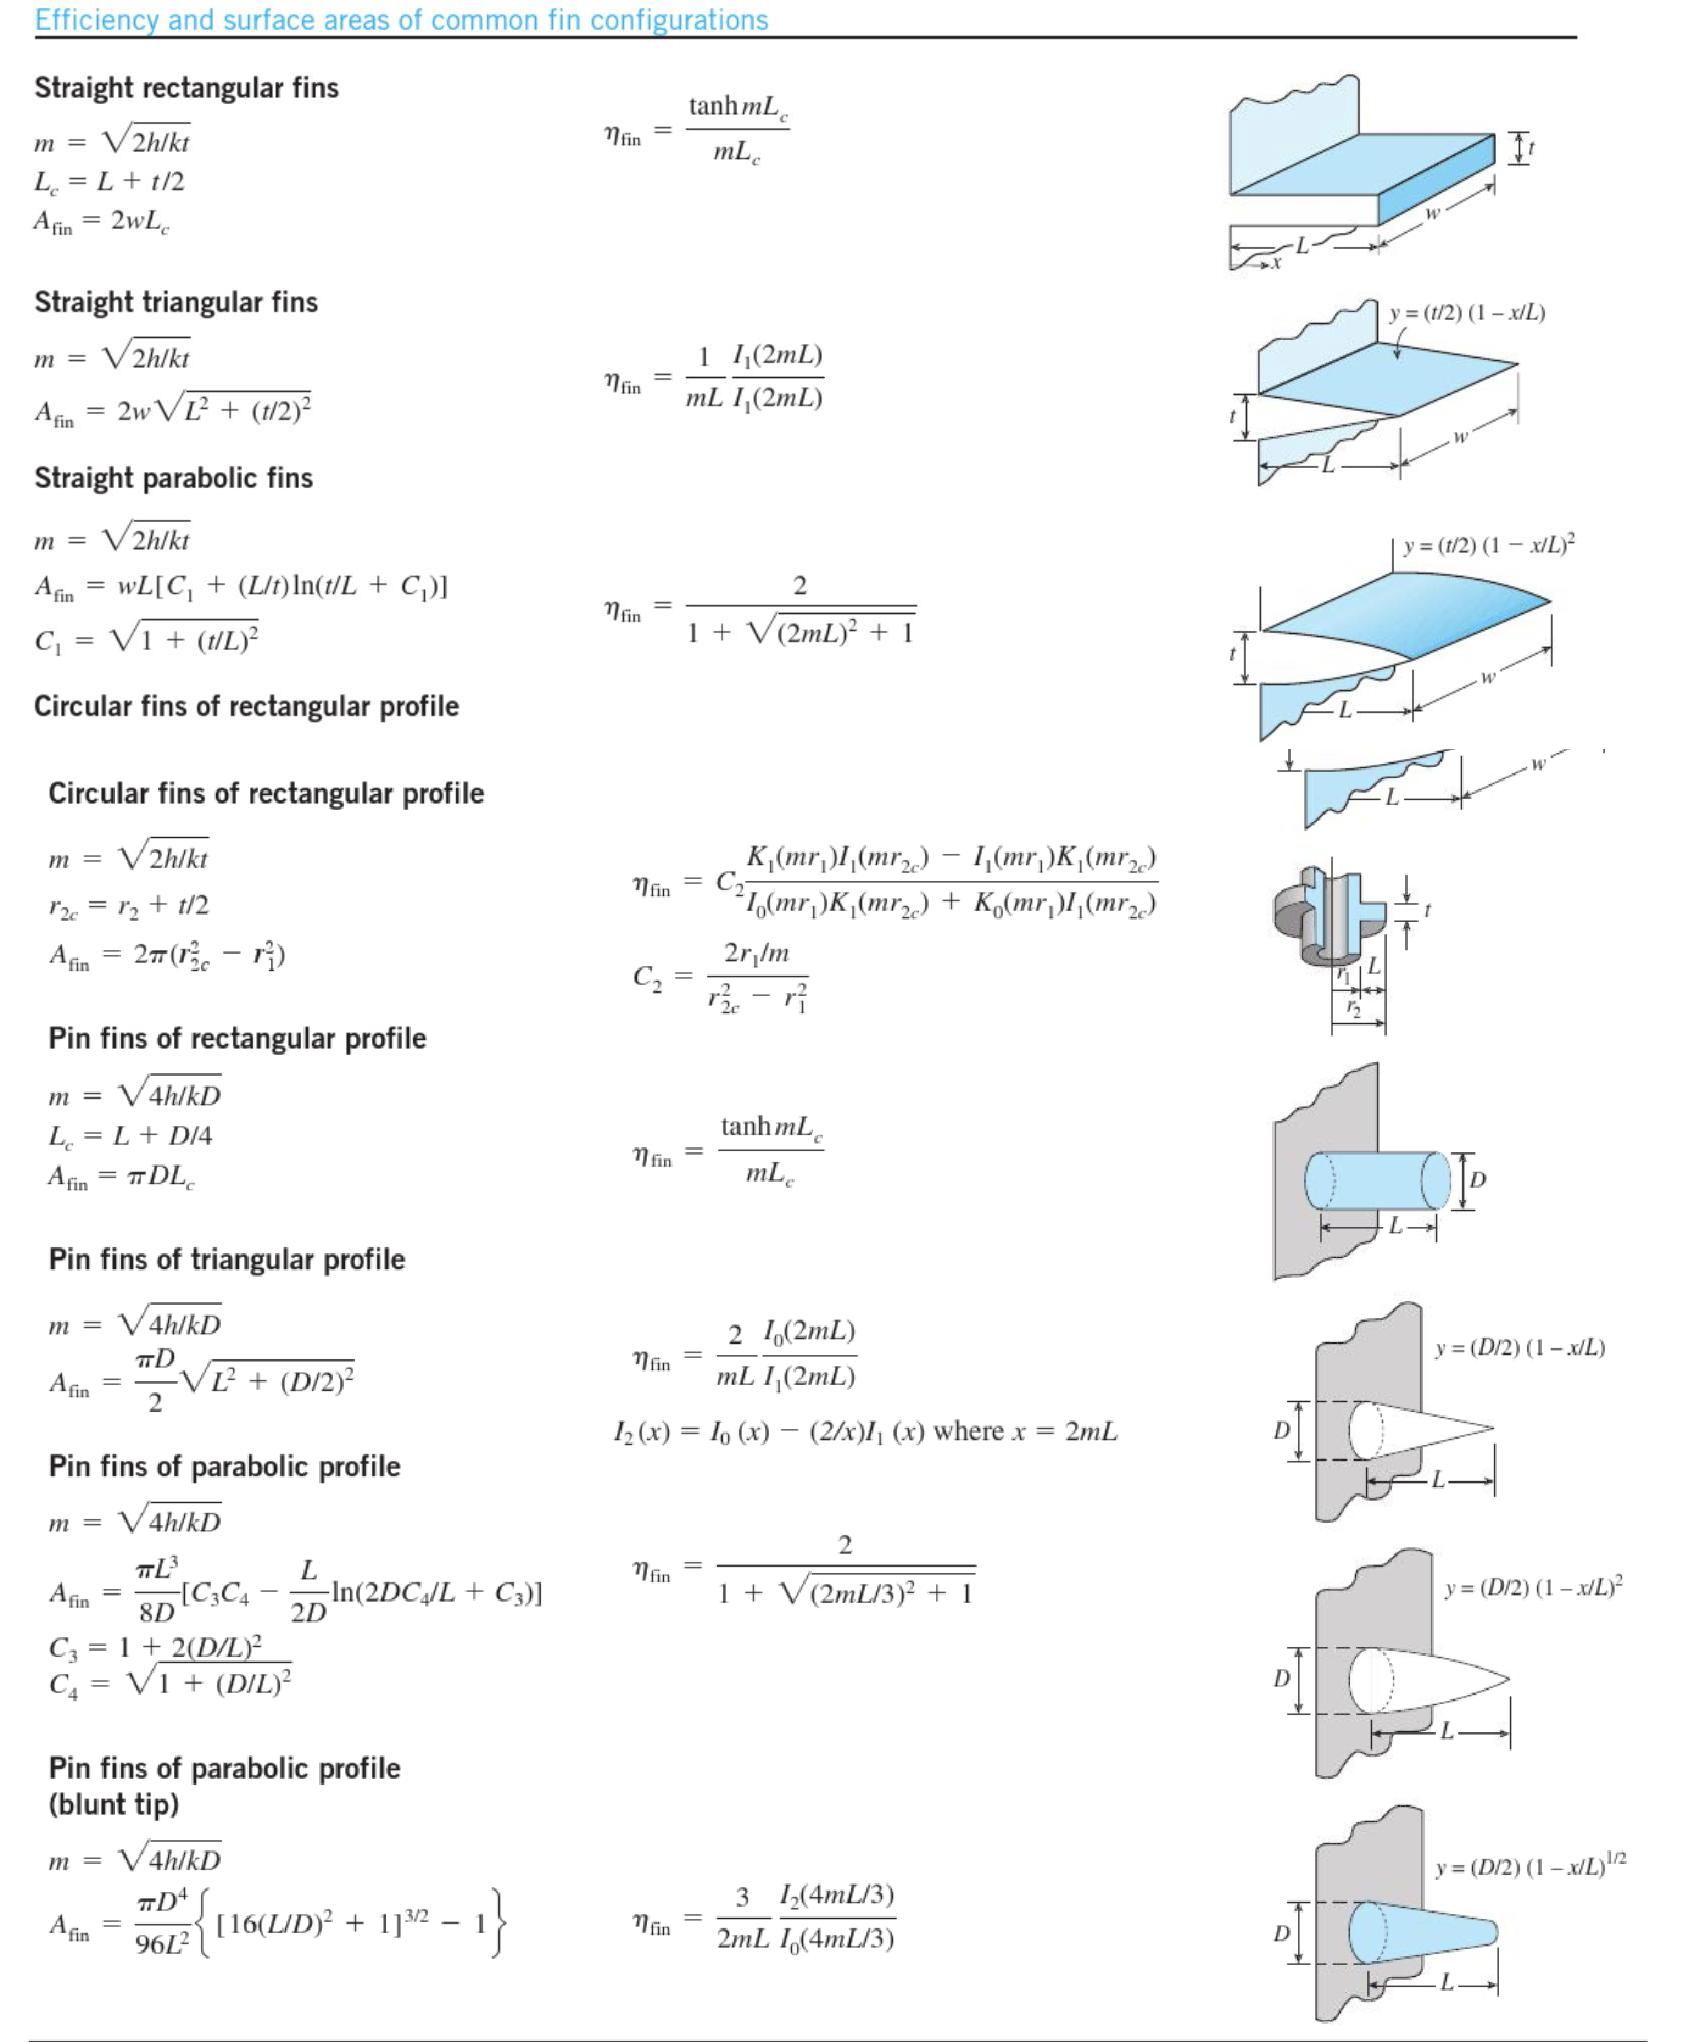
\includegraphics[width=1.0\linewidth]{images/fin_efficiency.png}
        \caption{Note $L_c$ is the corrected length.}
    \end{figure}
    \item \underline{\textbf{Fin effectiveness}}: measures the enhancement of heat transfer from fin. Defined as the ratio of \color{red} heat transfer rate from the fin of base area $A_b$ \color{black} over \color{blue} heat transfer rate from the surface of area $A_b$. \color{black}
    \begin{align*}
        \epsilon_{fin} &= \frac{\dot{Q}_{fin}}{\dot{Q}_{\text{no fin}}} = \frac{\dot{Q}_{fin}}{h A_b (T_b - T_{\infty})} \\
        &= \frac{A_{fin}}{A_b} \cdot \eta_{fin}
    \end{align*}
    \begin{figure}[H]
        \centering
        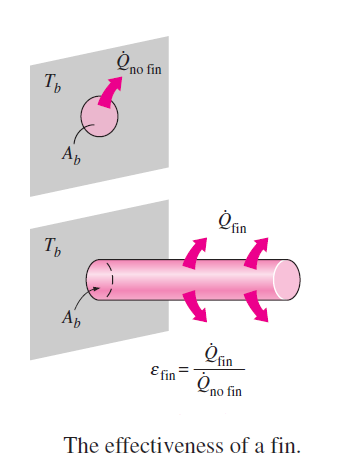
\includegraphics[width=0.5\linewidth]{images/fin_effectiveness.png}
    \end{figure}
    \begin{figure}[H]
        \centering
        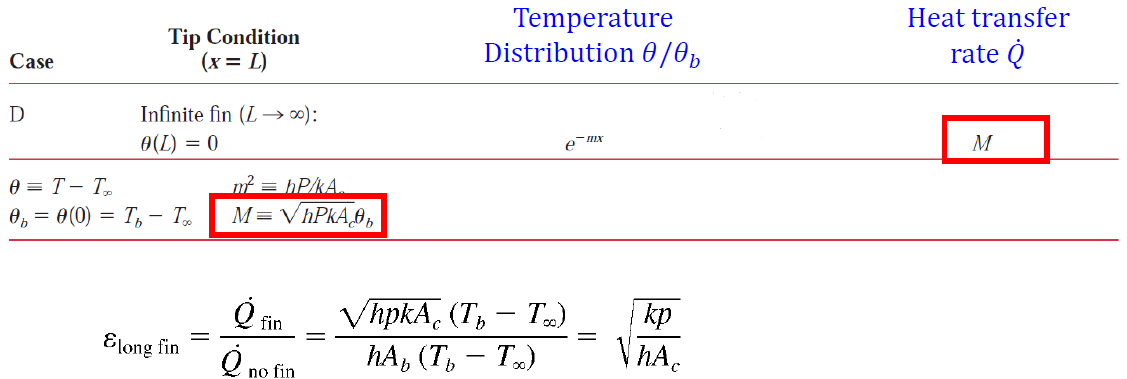
\includegraphics[width=1.0\linewidth]{images/fin_effectiveness_relation.png}
    \end{figure}
    \item $\epsilon_f \propto k$: made from metals usually;
    \item $\epsilon_f \propto \frac{1}{h}$: more effective in gases/natural convection;
    \item $\epsilon \propto \frac{P}{A_c}$: satisfied thin plate / slender fins
    \item \underline{\textbf{Fin arrays}}
    \begin{figure}[H]
        \centering
        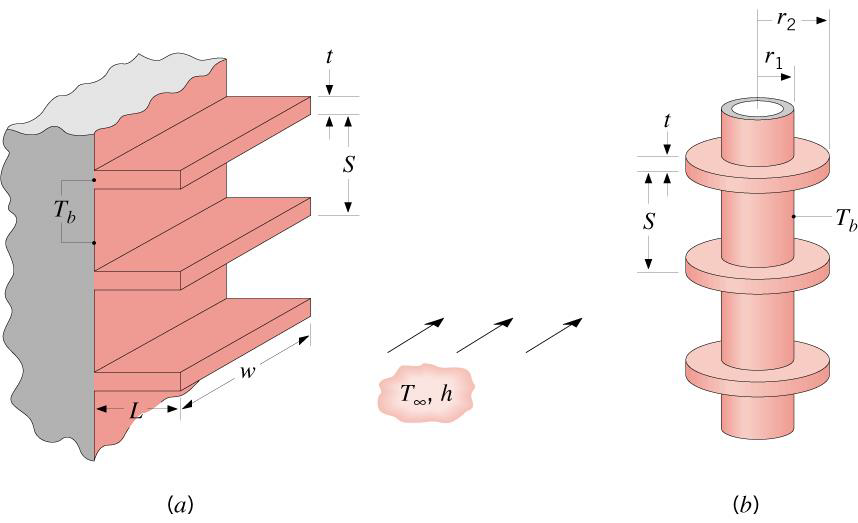
\includegraphics[width=1.0\linewidth]{images/fin_array_diagram.png}
    \end{figure}
    \begin{itemize}
        \item Total surface area:
        \begin{align*}
            A_t &= N A_f + A_b \\
            \text{where } N &= \text{number of fins,} \\
            A_b &= \text{area of exposed based (prime surface)}
        \end{align*}
        \item Total heat rate:
        \begin{align*}
            \color{blue} \dot{Q}_t &= \color{black} N \eta_f h A_f \theta_b + h A_b \theta_b \\
            &= h\left[N\eta_f A_f + (A_t - N A_f)\theta_b \right] \\
            &= h A_t \left[1 - \frac{NA_f}{A_t}(1-\eta_f)\right]
        \end{align*}
    \end{itemize}
\end{itemize}


\textbf{\underline{Fin efficiency read off from graph}}
\begin{figure}[H]
    \centering
    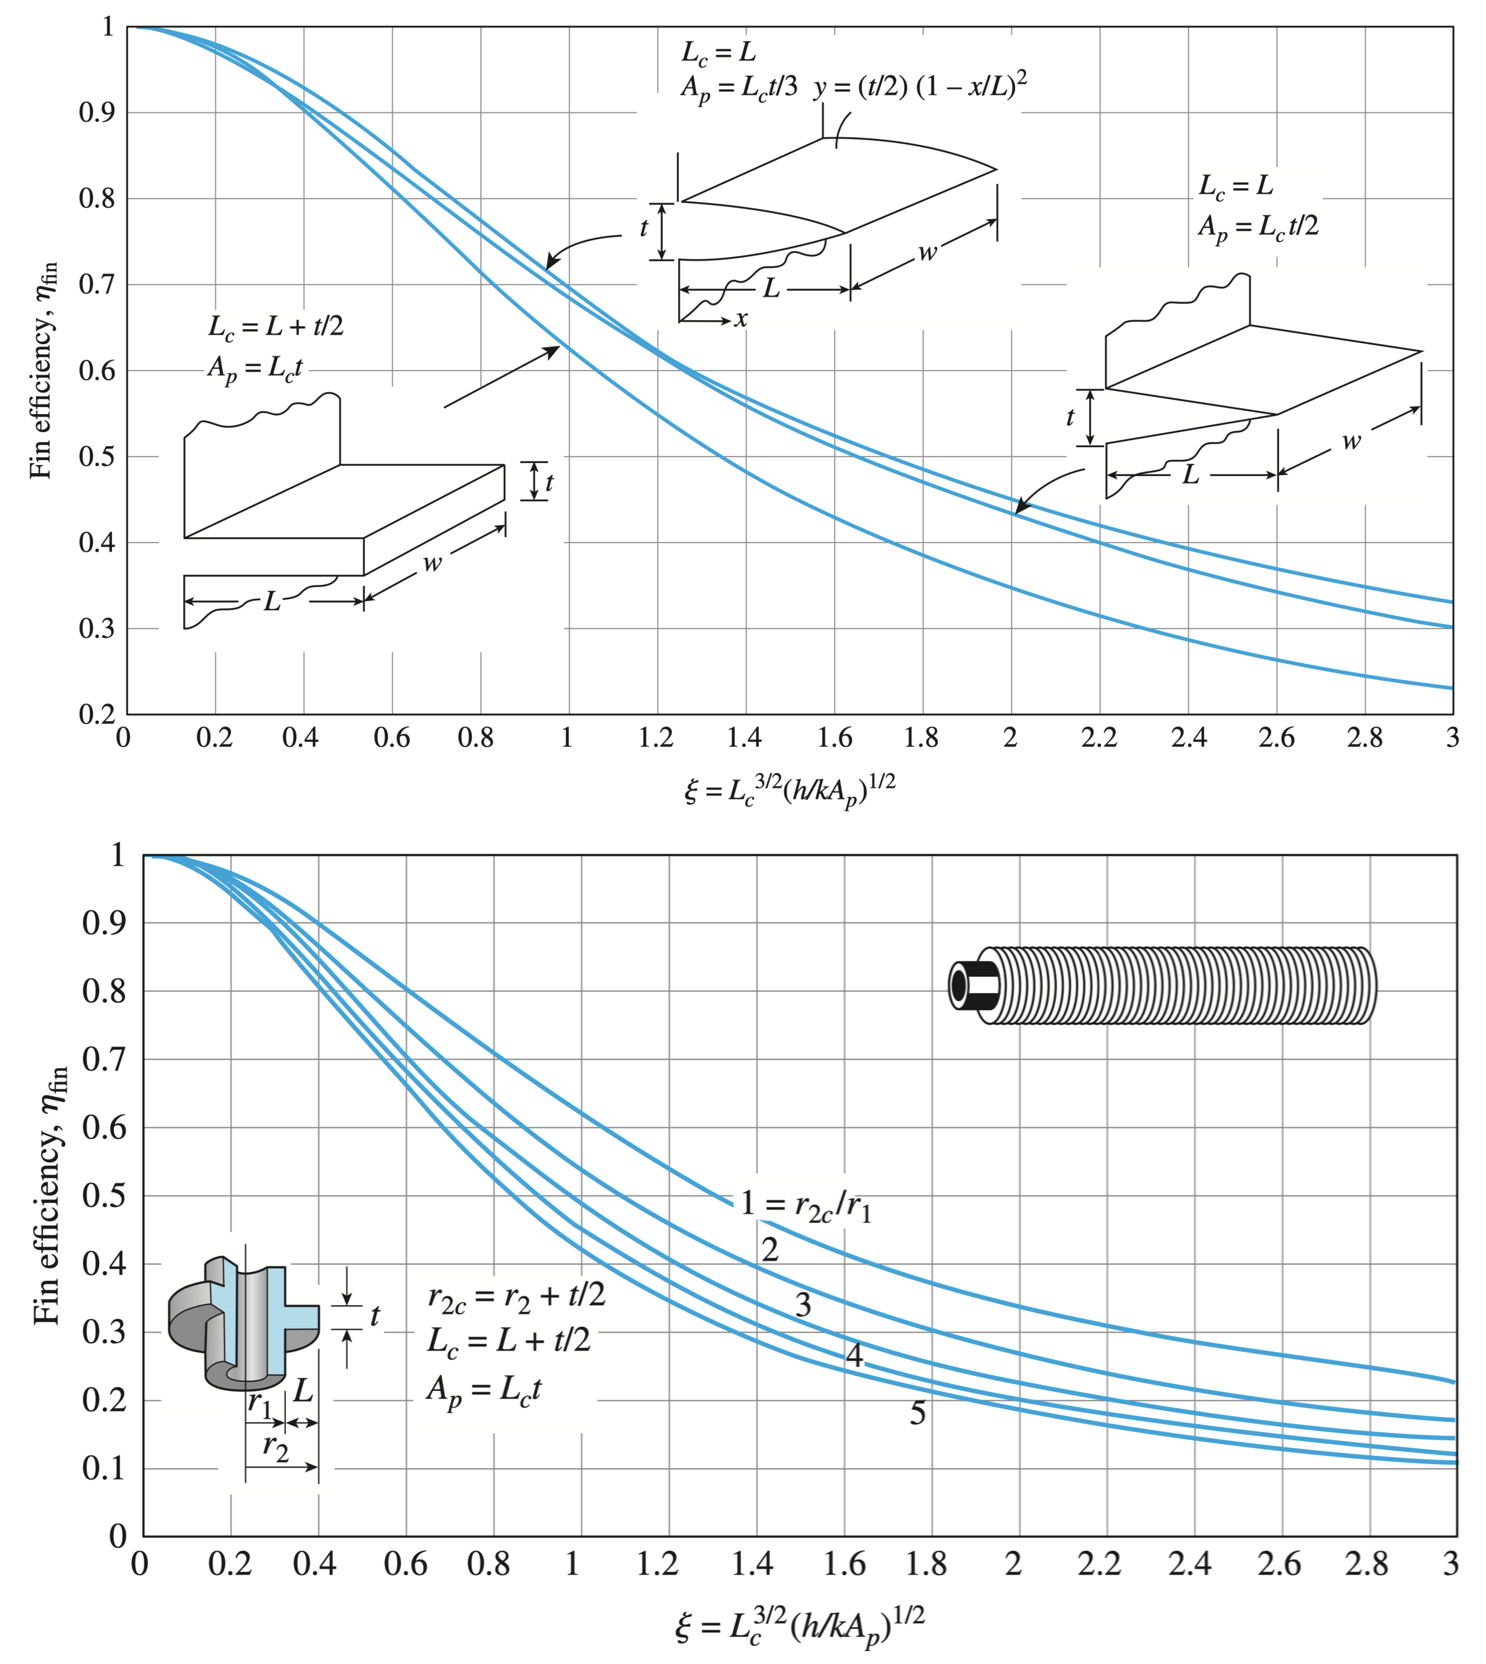
\includegraphics[width=1.0\linewidth]{images/Fin_efficiency_chart.png}
\end{figure}
Overall fin efficiency:
\begin{align*}
    R_{t,o} &= \frac{1}{\eta_o h A_t} \\
    \eta_o &= 1- \frac{N A_f}{A_t} (1-\eta_f)
\end{align*}

\textbf{\underline{Lumped Capacitance Method}}
\begin{figure}[H]
    \centering
    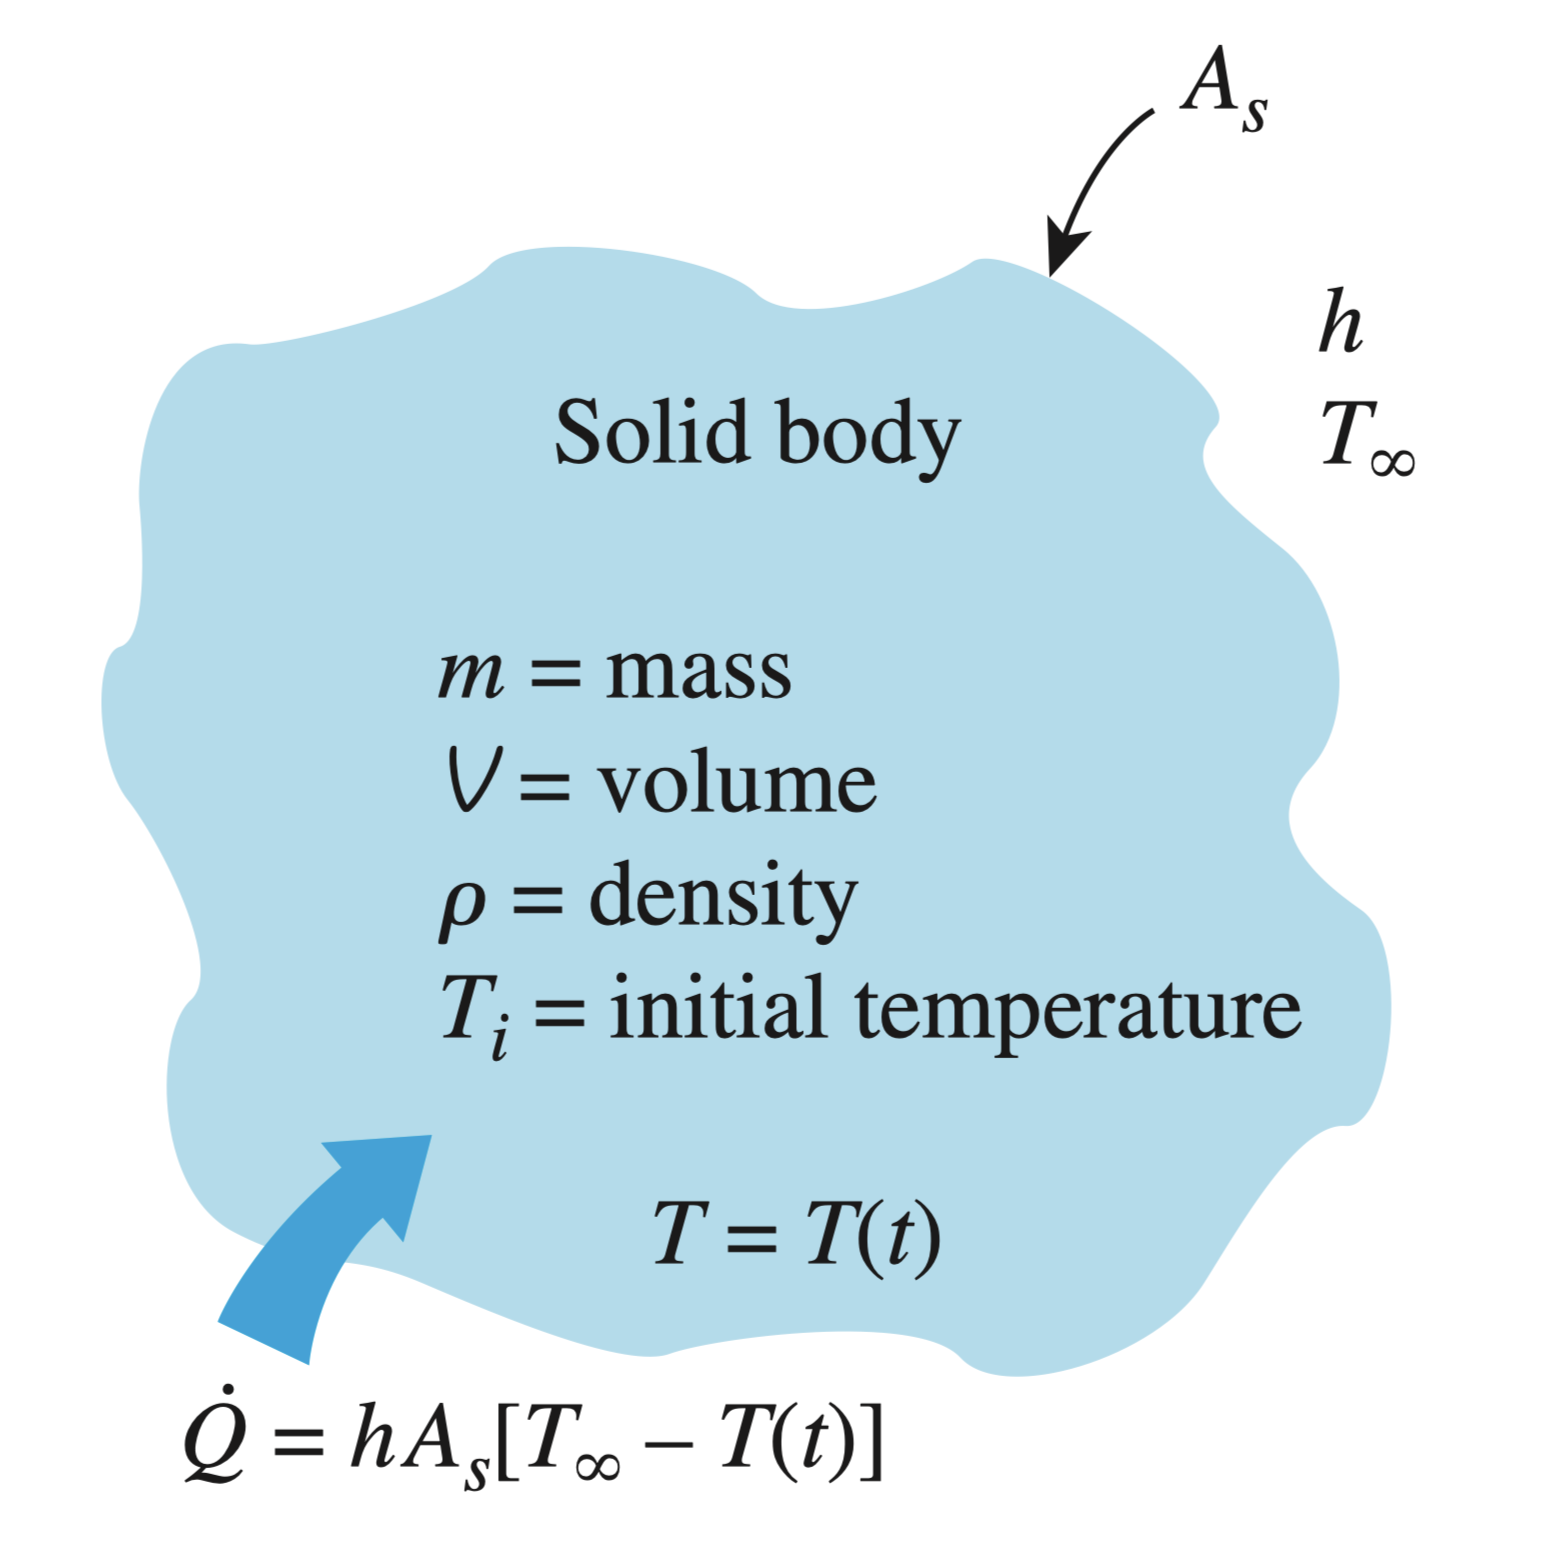
\includegraphics[width=0.55\linewidth]{images/lumped_system_analysis.png}
\end{figure}
\begin{itemize}
    \item Temperature of Body:
    \begin{align*}
        \frac{T(t) - T_{\infty}}{T_i - T_{\infty}} &= e^{-bt} \\
        \text{where } T(t) &= \text{temperature of body}\\
        b &= \frac{h A_s}{\rho V C_p} \; \text{[1/s]}
    \end{align*}
    \item Rate of heat transfer to/from environment at time t:
    \begin{equation*}
        \dot{Q}(t) = h A_s [T(t) - T_{\infty}] \;\; \; \text{[W]} 
    \end{equation*}
    \item Total amount of heat transferred between $\tau=0$ and $\tau = t$:
    \begin{equation*}
        Q = m C_p [T(t) - T_i] \;\; \; \text{[kJ]}
    \end{equation*}
    \item \textbf{\underline{Characteristic Length:}} 
    \begin{itemize}
        \item Less conservative but convenient for complex geometries: 
        \begin{equation*}
            L_c = \frac{V}{A_s} 
        \end{equation*}
        \item More conservative: calculated as the dimension corresponding to the max spatial temperature difference. Usually equivalent to \color{red} the furthest distance from surface to centroid. \color{black} 
    \end{itemize}
    \item Biot number: $\text{Bi} = \frac{h L_c}{k}$
    \begin{figure}[H]
        \centering
        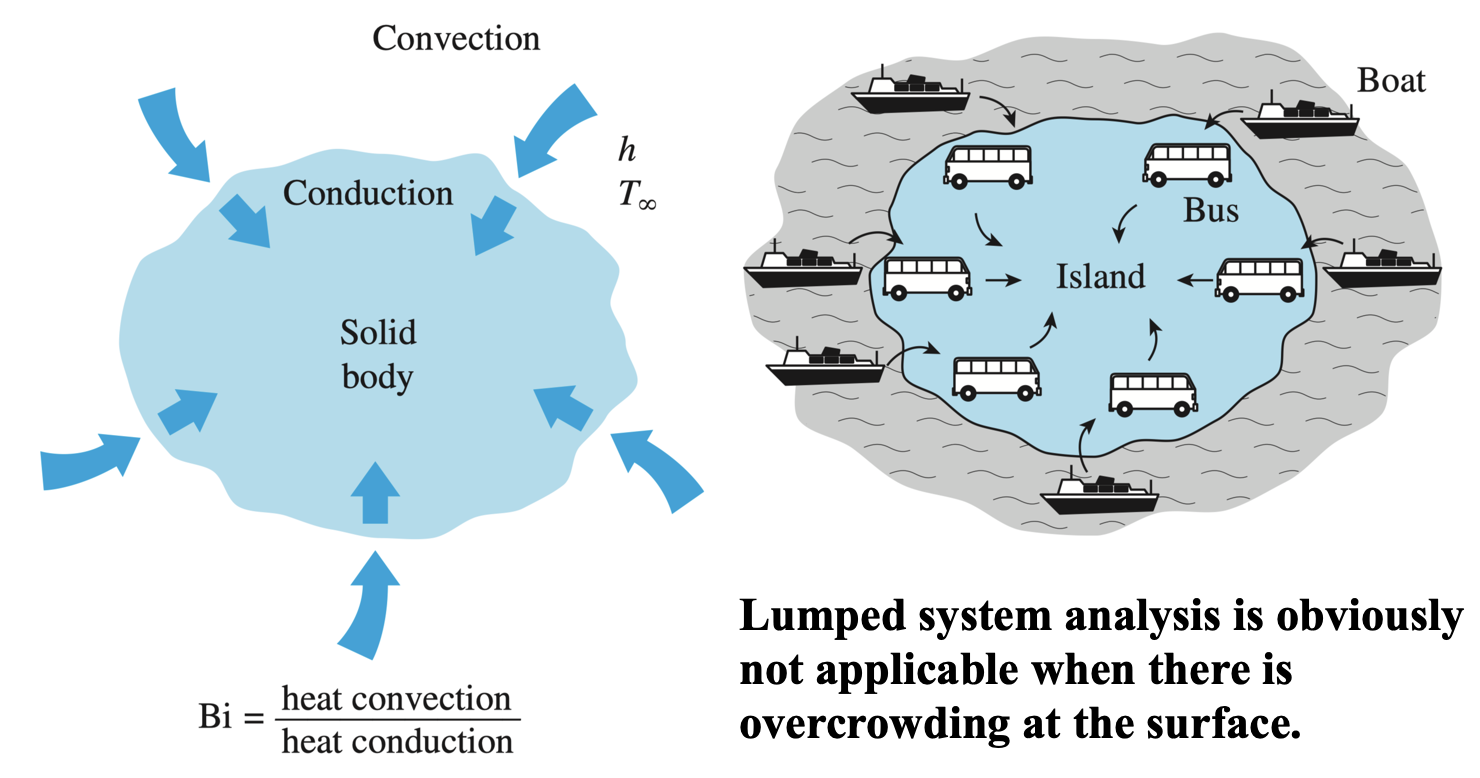
\includegraphics[width=1.0\linewidth]{images/Biot_number.png}
    \end{figure}
    \begin{itemize}
        \item Definition 1:
        \begin{align*}
            \text{Bi} &= \frac{h}{\left(\frac{k}{L_c}\right)}\cdot \frac{\Delta T}{\Delta T} \\
            &= \frac{\text{convection at the surface of body}}{\text{conduction within body}}
        \end{align*}
        \item Definition 2:
        \begin{align*}
            \text{Bi} &= \frac{\left(\frac{L_c}{k}\right)}{\left(\frac{1}{h}\right)} \\
            &= \frac{\text{conduction resistance within body}}{\text{convection resistance at the surface of body}}
        \end{align*}
    \end{itemize}
    \item \underline{Criterion for Applicability of LCM}:
    \begin{equation*}
        \text{Bi} \leq 0.1
    \end{equation*}
\end{itemize}

\underline{\textbf{\large Convections and External Flow}}
\begin{itemize}
    \item Convective heat transfer coefficient (defined at a single point):
    \begin{equation*}
        h \equiv \frac{-k_f \left(\frac{\partial T}{\partial y}\right)|_{y=0}}{T_s - T_{\infty}} \; \; \; \text{[W/$m^2\cdot K$]}
    \end{equation*}
    \item Average heat transfer coefficient (defined over the entire surface): 
    \begin{itemize}
        \item for a uniform surface temperature:
        \begin{equation*}
            \bar{h} = \frac{1}{A_s}\int_{A_s} h \, d A_s
        \end{equation*}
        \item for a flat plate in parallel flow:
        \begin{equation*}
            \bar{h} = \frac{1}{L} \int_{0}^{L} h \, dx
        \end{equation*}
    \end{itemize}
    
    
    \item \underline{\textbf{\large Nußelt number (non-dimensional)}}
    \begin{figure}[H]
        \centering
        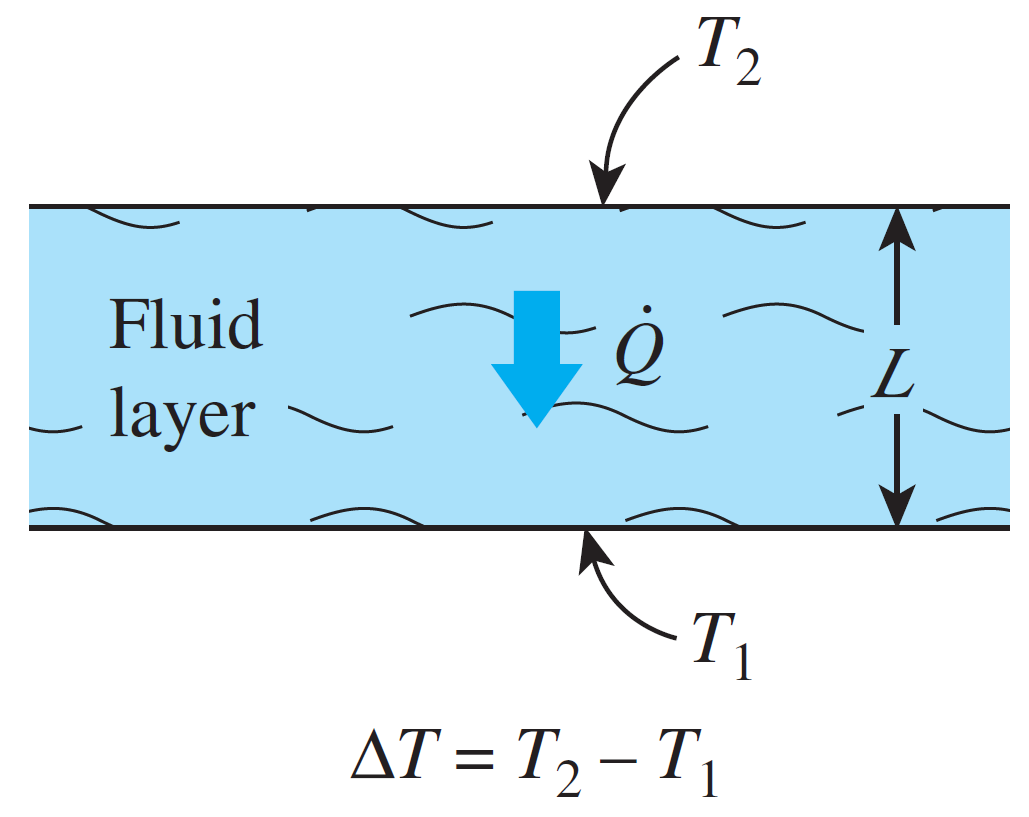
\includegraphics[width=0.55\linewidth]{images/Nusselt_number.png}
    \end{figure}
    \begin{equation*}
        \frac{q^{''}_{conv}}{q^{''}_{cond}} = \frac{h \Delta T}{k \left(\frac{\Delta T}{L_c}\right)} = \frac{hL_c}{k} = \text{Nu}
    \end{equation*}
    \item \textbf{Nu}: enhancement of heat transfer due to convection relative to conduction across the same fluid layer.
    \begin{itemize}
        \item $\text{Nu}>1$: (usually in laminar flows) the more effective convective heat transfer.
        \item $\text{Nu}\gg 1$: (usually in turbulent flows) 
        \item $\text{Nu}=1$: heat transfer is pure conduction
        \item $\text{Nu}<1$: Not possible. Convection always increases heat transfer.
    \end{itemize}
\end{itemize}
\section{Week 3}
The convection coefficient $h$ depends on
\begin{itemize}
    \item \color{blue}Fluid properties\color{black}
    \begin{itemize}
        \item density $\rho$
        \item viscosity $\mu$
        \item thermal conductivity $k$
        \item specific heat $c_p$
    \end{itemize}
    \item \color{blue} Surface geometry
    \item Flow conditions \color{black}
    \begin{itemize}
        \item \textbf{\underline{Laminar flow:}} smooth, orderly, low velocities, high viscosity. $h$ reduces as $\delta$ increases
        \item \underline{\textbf{Transition.}} Sudden increase in $h$ due to enhanced mixing.
        \item \underline{\textbf{Turbulent flow:}} chaotic, disorganized, high velocity, low viscosity. $h$ reduces as $\delta$ continues to increase
    \end{itemize}
    \begin{figure}[H]
        \centering
        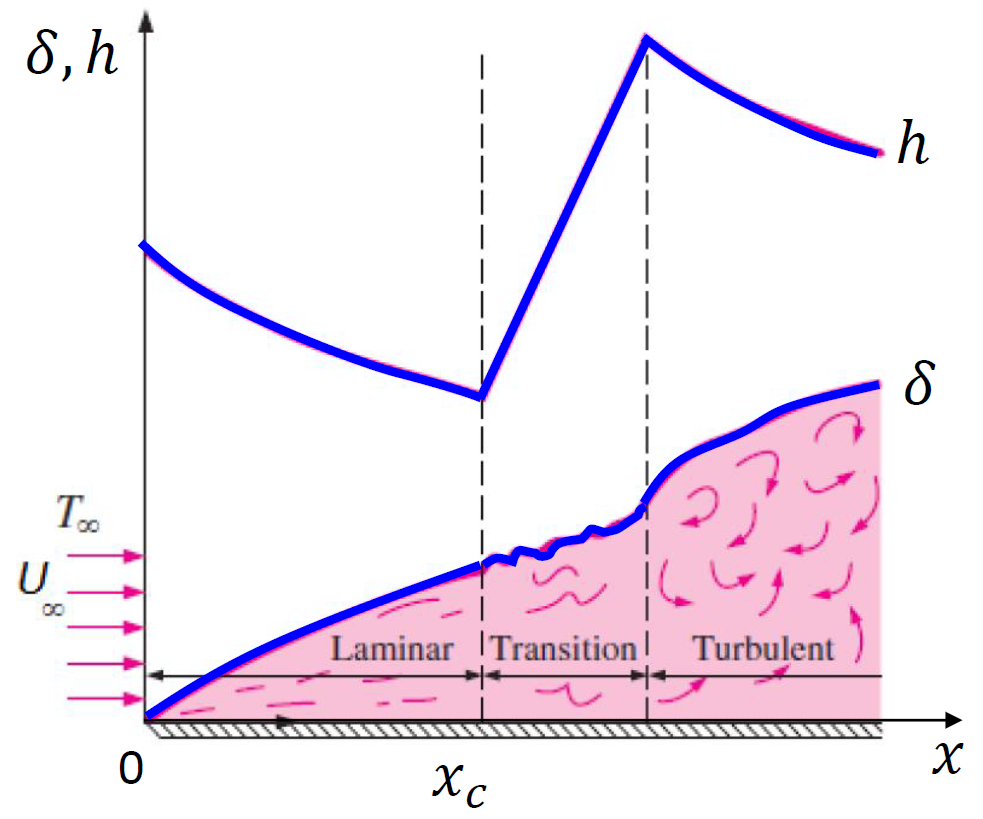
\includegraphics[width=0.8\linewidth]{images/convection_vs_Renold.png}
    \end{figure}
\end{itemize}

\underline{\textbf{\large Reynolds number:}}
\begin{figure}[H]
    \centering
    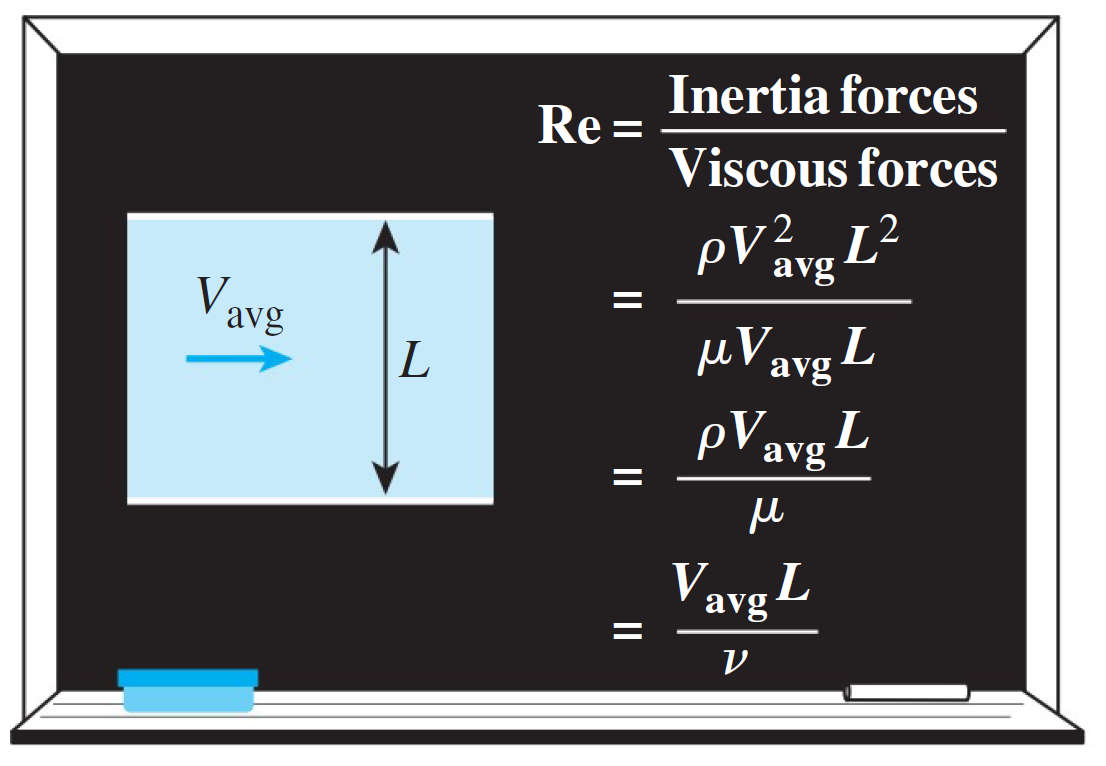
\includegraphics[width=0.8\linewidth]{images/Renolds_Number.png}
\end{figure}
\begin{itemize}
    \item Critical Reynolds number: transition from laminar to turbulent
    \begin{equation*}
        \text{Re}_{x,c} \approx 5\times 10^5
    \end{equation*}
    \begin{itemize}
        \item Transition can \color{red} be advanced \color{black} if the surface roughness is high;
        \item Transition can \color{red} be delayed \color{black} if there are suction / vortex generators 
    \end{itemize}
    \item Characteristic Length
\end{itemize}
\textbf{\underline{Prandtl Number}}
\begin{equation*}
    \text{Pr} = \frac{c_p \mu}{k} = \frac{v}{\alpha}
\end{equation*}
\begin{itemize}
    \item \color{red}Pr \color{black} is a ratio of \color{blue} momentum diffusivity \color{black} (kinematic viscosity, $v$) to \color{blue} thermal diffusivity \color{black} ($\alpha$)
    \item \color{red} Pr \color{black} is a measure of the \color{blue} relative effectiveness of momentum \color{black} and \color{blue} thermal energy transport \color{black} by diffusion in the velocity and thermal boundary layers.
    \begin{align*}
        \text{Pr} &\approx 1 \; \; \text{momentum and heat dissipation comparable} \\
        \text{Pr} &< 1 \;\; \text{heat diffuses quickly (typical in air, liquid, metals)} \\
        \text{Pr} &> 1 \;\;\text{heat diffuses slowly (typical in oils, water)}
    \end{align*}
\end{itemize}
\textbf{\underline{Principle of Similarity}}
\begin{itemize}
    \item Despite different length, different velocities, and different fluids, the two situations are compatible if $Re_1=Re_2$, $Pr_1 = Pr_2$, $Nu_1 = Nu_2$.
\end{itemize}

\textbf{\underline{Film Temperature}}
\begin{itemize}
    \item average temperature between $T_{\infty}$ and $T_{s}$: 
    \begin{equation*}
        T_f = \frac{T_{\infty}+T_{f}}{2}
    \end{equation*}
\end{itemize}

\textbf{\Large \underline{External Flow}}

\begin{itemize}
    \item Empirical form of Nußelt number: 
    \begin{equation*}
        \text{Nu}=C\cdot \text{Re}^{m}_{x}\cdot \text{Pr}^{n}
    \end{equation*}
    C, m, and n are often independent of the nature of fluid. C depends on geometry / flow.  
    \item Case 1: \color{red} Flat Plate \color{black}
    \begin{itemize}
        \item Local coefficient \color{blue} (isothermal surfaces) \color{black}
        \begin{align*}
            \text{Laminar: }\; \text{Nu} &= \frac{hx}{k} = 0.332 \text{Re}_{x}^{1/2} \text{Pr}^{1/3} \\
            Pr &> 0.6 \\
            \text{Re}_{x} &< 5\times 10^5\\
            \text{Turbulent: }\; \text{Nu} &= \frac{hx}{k} = 0.0296 \text{Re}_{x}^{0.8} \text{Pr}^{1/3} \\
            0.6 &< Pr < 60 \\
            5\times 10^5 &< \text{Re}_{x} < 10^7
        \end{align*}
        \item Average coefficient
        \begin{align*}
            \text{Laminar: }\; \overline{\text{Nu}}_L &= \frac{\bar{h}L}{k} = 0.664 \text{Re}_{L}^{1/2} \text{Pr}^{1/3} \\
            \text{Turbulent: }\; \overline{\text{Nu}}_L &= \frac{\bar{h}L}{k} = 0.037 \text{Re}_{L}^{0.8}
        \end{align*}
        \item Local coefficient \color{blue} (uniform heat flux) \color{black}
        \begin{align*}
            \text{Laminar: }\; \text{Nu} &= \frac{hx}{k} = 0.453 \text{Re}_{x}^{1/2} \text{Pr}^{1/3} \\
            Pr &> 0.6 \\
            \text{Re}_{x} &< 5\times 10^5\\
            \text{Turbulent: }\; \text{Nu} &= \frac{hx}{k} = 0.0308 \text{Re}_{x}^{0.8} \text{Pr}^{1/3} \\
            0.6 &< Pr < 60 \\
            5\times 10^5 &< \text{Re}_{x} < 10^7
        \end{align*}
        \item Flow composed of both laminar and turbulent regions:
        \begin{align*}
            \overline{\text{Nu}}_L &= \left(0.037\, \text{Re}_{L}^{4/5}-A\right)\, \text{Pr}^{1/3} \\
            A &= 0.037 \, \text{Re}^{4/5}_{x,c} - 0.664 \, \text{Re}^{1/2}_{x,c} 
        \end{align*}
        \begin{table}[H]
            \centering
            \begin{tabular}{|l|l|l|l|}
            \hline
            \textbf{$\text{Re}_{x,c}$}   & \textbf{$10^5$} & \textbf{$5\times 10^5$} & \textbf{$10^6$} \\ \hline
            $A$                          & 160             & 871                     & 1671            \\ \hline
            $\overline{\text{Nu}}_L$     & 2645            & 2014                    & 1303            \\ \hline
            $\bar{h}_L$ (W/$m^2\cdot K$) & 79.2            & 60.2                    & 39              \\ \hline
            $q'$ (W/m)                   & 17,420          & 13,270                  & 8595            \\ \hline
            \end{tabular}
        \end{table}
        \item Weighted average of surface temperature
        \begin{align*}
            \overline{T_s - T_{\infty}} &= \frac{1}{L} \int_{0}^{L} \left(T_s - T_{\infty}\right)\, dx \\
            &= \frac{q^{''}_{s}}{L} \int_{0}^{L} \frac{x}{k \text{Nu}_x} \, dx
        \end{align*}
    \end{itemize}
    \item Case 2: \color{red} Cylinder \color{black}
    \begin{align*}
        \text{Re}_D &\equiv \frac{\rho V D}{\mu} = \frac{VD}{v} \\
        \overline{\text{Nu}}_D &= \frac{\bar{h}D}{k}
    \end{align*}
    \begin{itemize}
        \item Churchill and Bernsein's equation:
        \begin{equation*}
            \text{Criterion of application:}\;\;\text{Re}\cdot \text{Pr} > 0.2
        \end{equation*}
    \end{itemize}
\end{itemize}
\begin{equation*}
            \overline{\text{Nu}}_D = 0.3 + \frac{0.62\, \text{Re}_D^{1/2}\, \text{Pr}^{1/3}}{\left(1+(\frac{0.4}{\text{Pr}})^{2/3}\right)^{1/4}} \left[1+\left(\frac{\text{Re}_D}{282000}\right)^{5/8}\right]^{4/5}
        \end{equation*}
\begin{figure}[H]
    \centering
    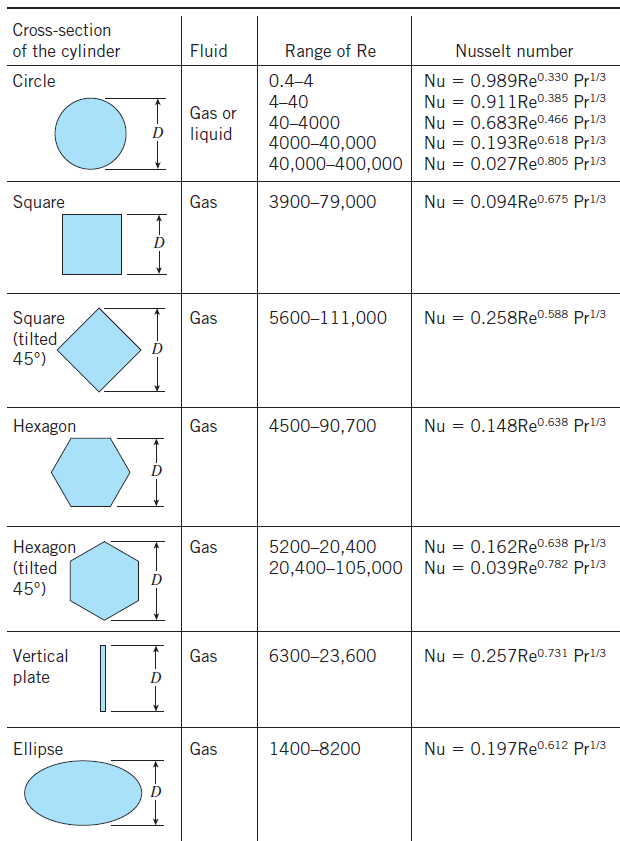
\includegraphics[width=1.0\linewidth]{images/Nusselt_Number_Cylinder.png}
\end{figure}

\begin{itemize}
    \item Case 3: \color{red} Sphere \color{black}
    
    Whitaker's correlation:
    \begin{equation*}
        \overline{\text{Nu}}_D = 2 + \left(0.4\text{Re}_{D}^{1/2}+0.06\text{Re}_{D}^{2/3}\right)\text{Pr}^{0.4}\left(\frac{\mu_{\infty}}{\mu_s}\right)^{1/4}
    \end{equation*}
    Limits of application (all properties are evaluated at $T_{\infty}$, except $\mu_s$ which is at $T_s$):
    \begin{align*}
        3.5 &< \text{Re}_D < 7.6 \times 10^5 \\
        0.71 &< \text{Pr} < 380 \\
        1 &< \frac{\mu_{\infty}}{\mu_s} < 3.2
    \end{align*}
\end{itemize}

\begin{itemize}
    \item Case 4: \color{red} Flow across tube banks \color{black}
    \begin{figure}[H]
        \centering
        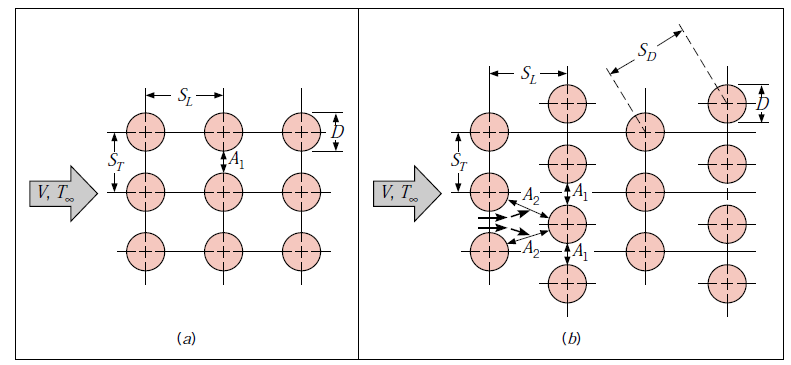
\includegraphics[width=1.0\linewidth]{images/tube_bank.png}
    \end{figure}
    \begin{itemize}
        \item Aligned:
        \begin{equation*}
            V_{max} = V \frac{S_T}{S_T-D}
        \end{equation*}
        \item Staggered:
        \begin{align*}
            V_{max} &= V \frac{S_T}{S_T - D} \; \; \text{if 2$A_2>A_1$} \\
            V_{max} &= V \frac{S_T}{2(S_D - D)}\;\; \text{if 2$A_2<A_1$}
        \end{align*}
        \item Average Nusselt Number for an isothermal array:
        \begin{align*}
            \overline{\text{Nu}}_D &= \frac{hD}{k} = C \,\text{Re}^m_D \, \text{Pr}^n \left(\frac{\text{Pr}}{\text{Pr}_s}\right)^{0.25}\\
            \text{Nu}_{D,N_{L<16}} &= F \, \text{Nu}_D
        \end{align*}
        Look up Table 7.2 to find $C$, $m$, and $n$, and look up Table 7.3 for correction factor $F$.
    \end{itemize}
\end{itemize}
\begin{figure}[H]
    \centering
    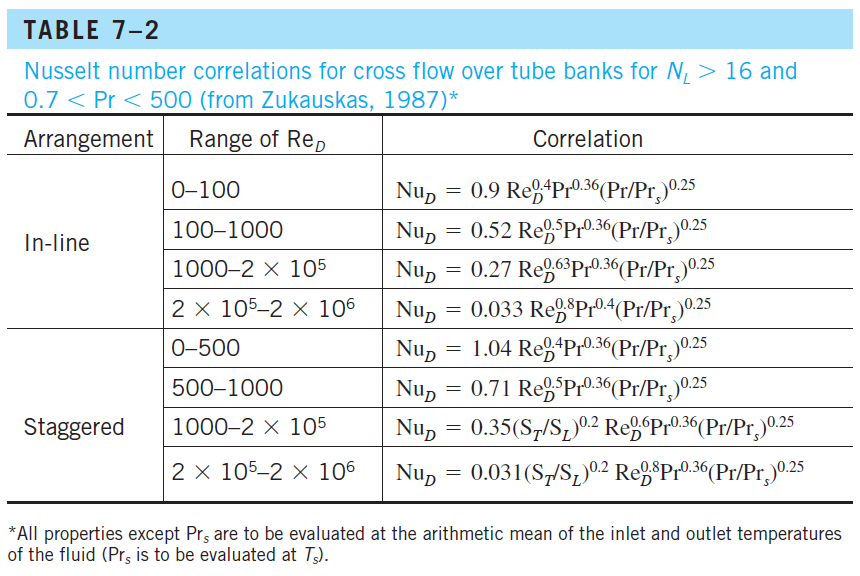
\includegraphics[width=1.0\linewidth]{images/Table_7_2.png}
    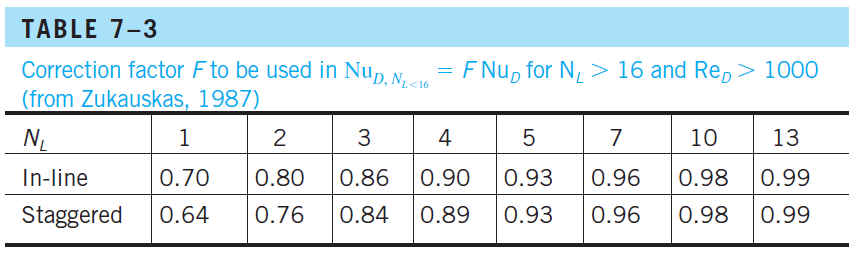
\includegraphics[width=1.0\linewidth]{images/Table_7_3.png}
\end{figure}

\underline{\textbf{\large Internal Flows}}
\begin{itemize}
    \item Hydrodynamic entrance region
    \begin{align*}
        L_{\text{h,laminar}} &\approx 0.05 \cdot \text{Re} \cdot D \\
        L_{\text{h,turbulent}} &\approx 10D
    \end{align*}
    \begin{figure}[H]
        \centering
        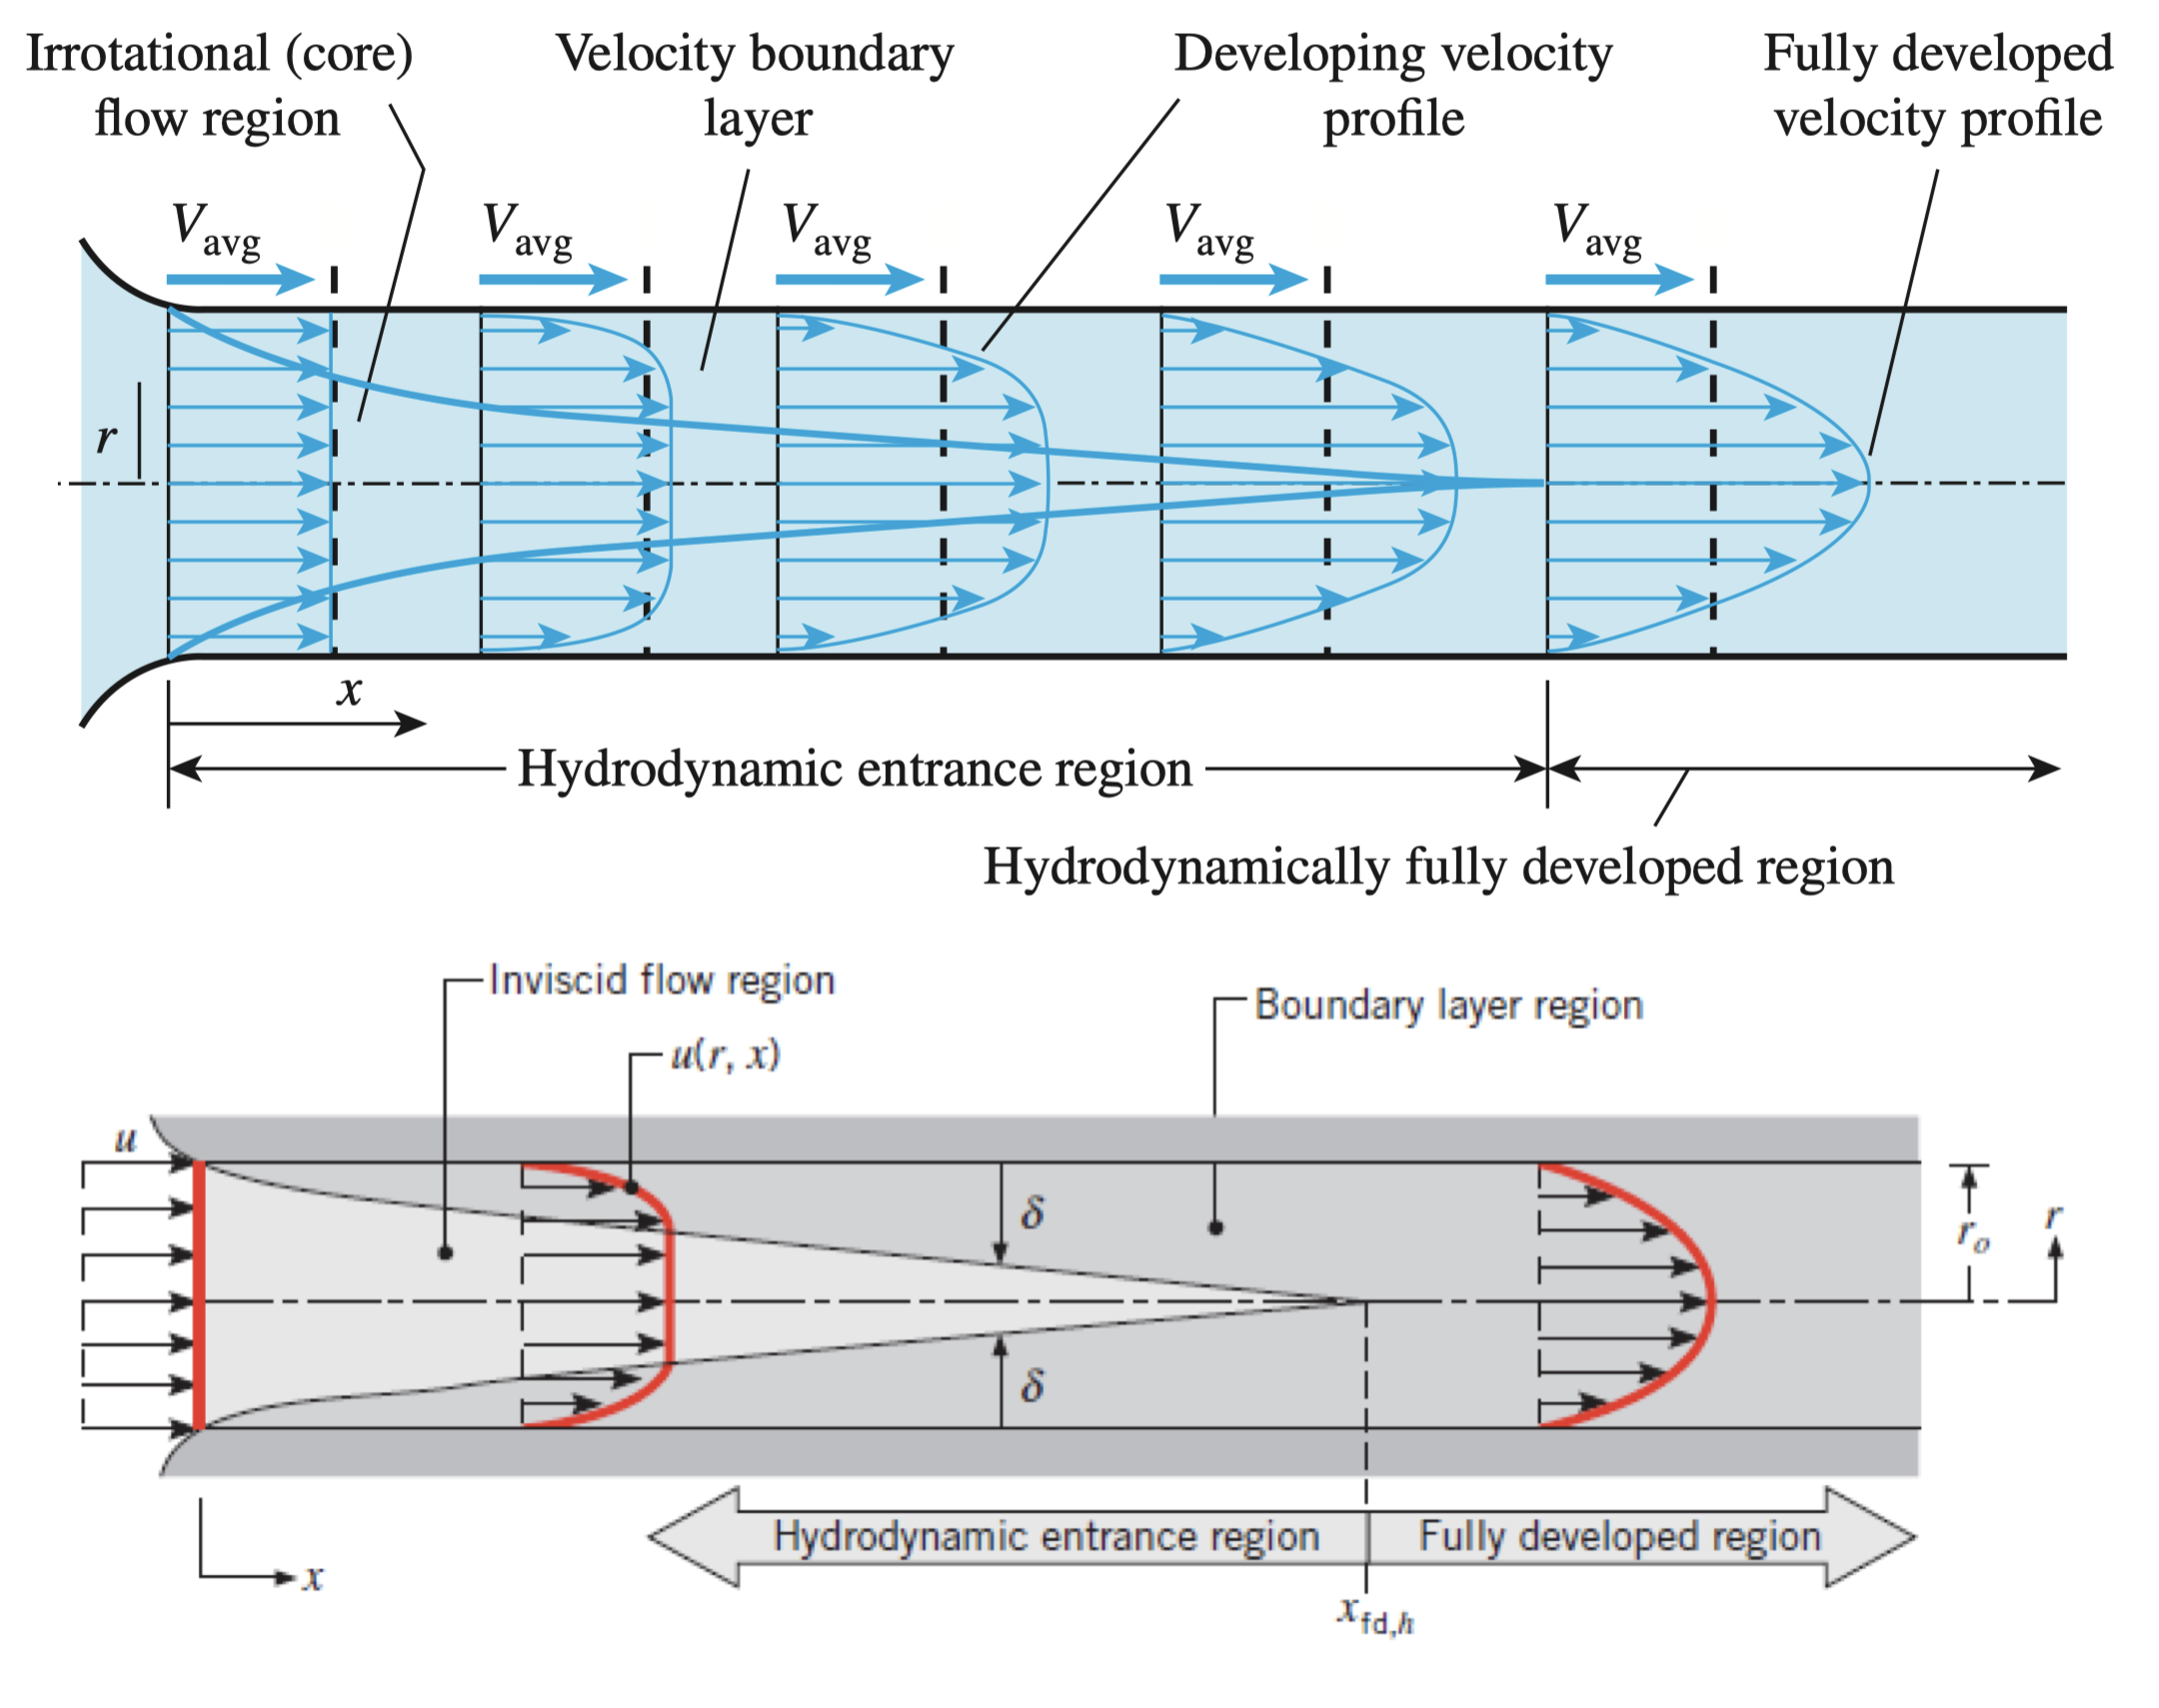
\includegraphics[width=1.0\linewidth]{images/hydrodynamic_entrance.png}
    \end{figure}
    \item Thermal entrance region
        \begin{align*}
            L_{\text{t,laminar}} &\approx 0.05 \cdot \text{Re} \cdot \text{Pr} \cdot D = \text{Pr}\cdot L_{\text{h,laminar}}
        \end{align*}
        \begin{figure}[H]
            \centering
            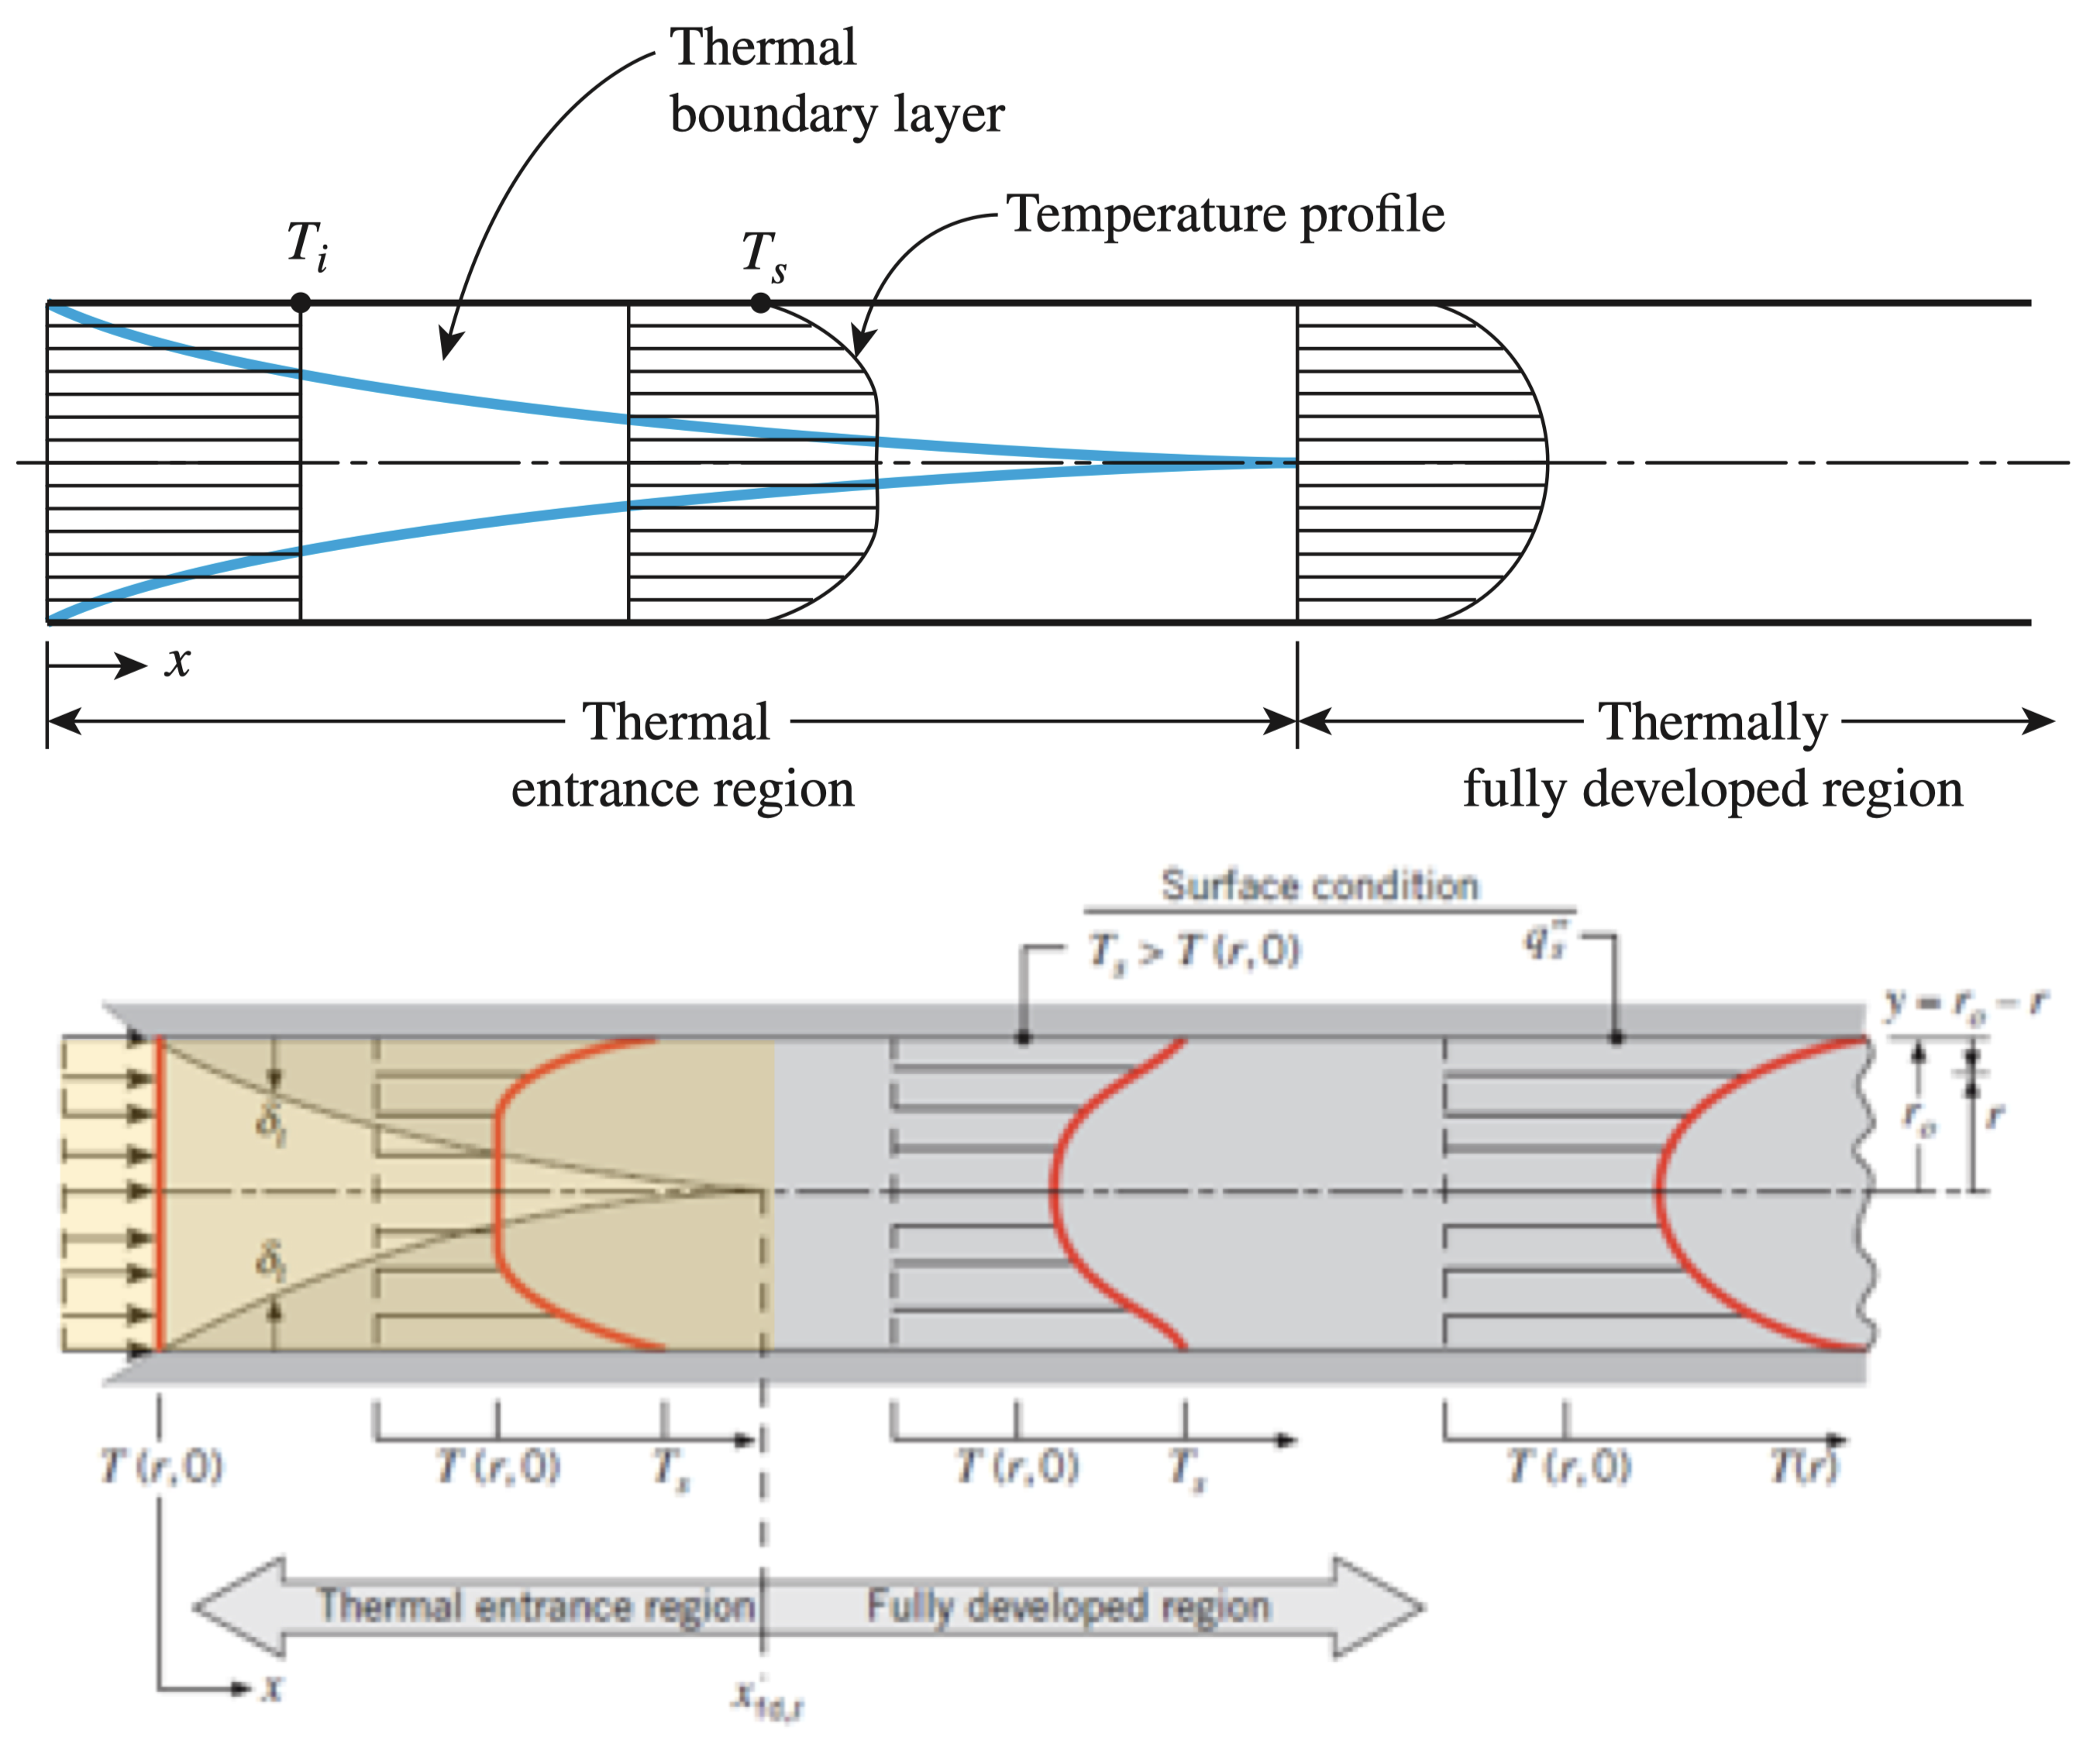
\includegraphics[width=1.0\linewidth]{images/thermal_entrance.png}
        \end{figure}
\end{itemize}
\begin{itemize}
        \item Reynolds number:
        \begin{align*}
            \text{Re}_D &= \frac{\rho u_m D_h}{\mu} \\
            \text{where } D_h &= \frac{4\cdot\text{crosssection area}}{perimeter} = \frac{4A_c}{P}
        \end{align*}
        \color{red}\underline{For a circular pipe:}\color{black}
        \begin{align*}
            \text{Re}_D &= \frac{\rho u_m D}{\mu} = \frac{\rho D}{\mu} \left(\frac{\dot{m}}{\rho (\pi D^2 /4)}\right) = \frac{4\dot{m}}{\mu \pi D}
        \end{align*}
        \item \color{red}\underline{For an annulus (ring circular pipe):}\color{black}
        \begin{equation*}
            D_h = D_o - D_i
        \end{equation*}
        \begin{align*}
            \text{Re}_D &= \frac{\rho u_m D_h}{\mu} \\
            &= \frac{\rho (D_o - D_i)}{\mu} \times \frac{\dot{m}}{\rho \pi (D_o^2 - D_i^2)/4} \\
            &= \frac{4 \dot{m}}{\pi (D_o + D_i)\mu }
        \end{align*}
        \begin{figure}[H]
            \centering
            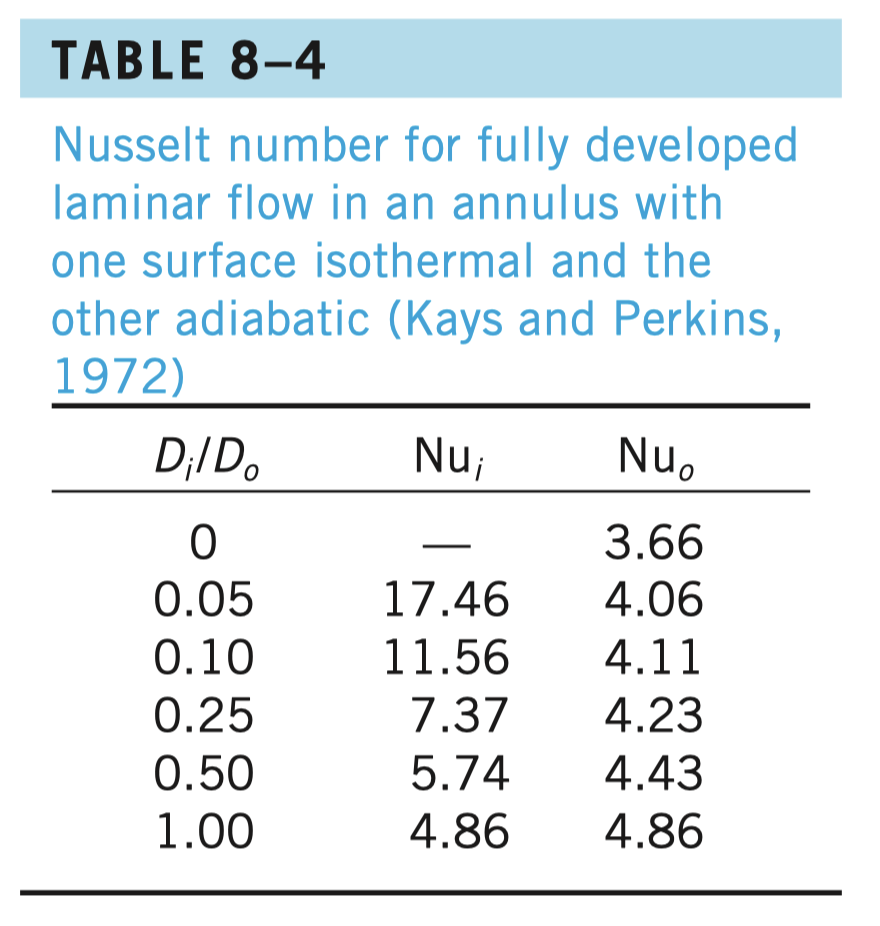
\includegraphics[width=0.7\linewidth]{images/internal_flow_annulus.png}
        \end{figure}
        \item Onset of turbulence occurs at a critical Reynolds number of:
        \begin{equation*}
            \text{Re}_{D,c} \approx 2300
        \end{equation*}
        \item Fully turbulent conditions exist for: 
        \begin{equation*}
            \text{Re}_D\approx 10000
        \end{equation*}
\end{itemize}
\textbf{\underline{\large Mean Temperature}}
\begin{itemize}
    \item Constant surface heat flux
    \begin{align*}
        \dot{Q} &= q^{''}_{s}A_s = \dot{m} c_p (T_e - T_i) \\
        T_m &= T_i + \frac{P q_{s}^{''}}{\dot{m}c_p} x \\
        T_s &= T_m + \frac{q_{s}^{''}}{h}
    \end{align*}
    \item Constant surface temperature
    \begin{align*}
        \Delta T &\equiv T_s - T_m \\
        \Delta T_{lm} &= \frac{\Delta T_e - \Delta T_i}{\ln(\Delta T_e / \Delta T_i)} \\
        \dot{Q} &= \overline{h} A_s \Delta T_{lm}
    \end{align*}
    where $\Delta T_{lm}$ is the log-mean temperature difference.
\end{itemize}

\textbf{\underline{\large Fully Developed Flow}}
\begin{itemize}
    \item For hydraulically and thermally fully-developed \color{blue} laminar flow \color{black} in a \color{blue} circular tube \color{black}:
    \begin{enumerate}
        \item Constant surface heat flux $q_{s}^{''}$:
        \begin{equation*}
            \text{Nu}_D = \frac{hD}{k} = 4.36 \; \; \text{constant everywhere}
        \end{equation*}
        \item Constant surface temperature $T_s$:
        \begin{equation*}
            \text{Nu}_D = \frac{hD}{k} = 3.66 \;\;\text{constant everywhere}
        \end{equation*}
    \end{enumerate}
    \begin{figure}[H]
            \centering
            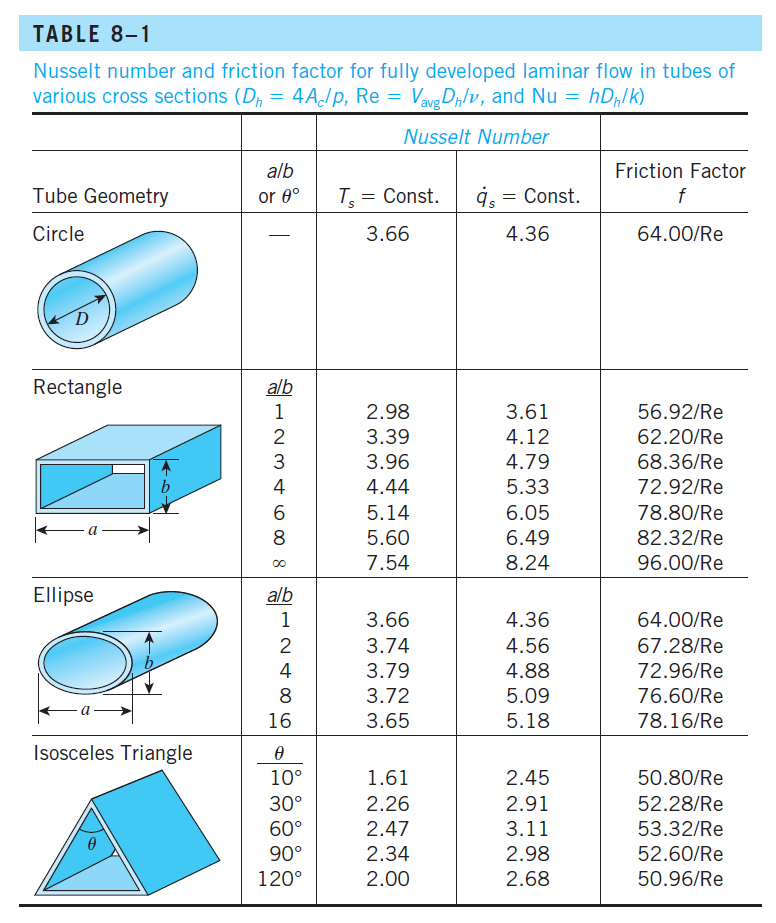
\includegraphics[width=1.0\linewidth]{images/Table_8_1.png}
    \end{figure}
    Note: to determine $h$, evaluate $k$ at $T_m$
    \item For  hydraulically and thermally fully-developed \color{blue} turbulent flow \color{black} in a \color{blue} circular tube \color{black}:
    \begin{enumerate}
        \item For a smooth surface and fully turbulent conditions:
        \begin{align*}
            \text{Nu}_D &= 0.023 \, \text{Re}_D^{4/5} \, \text{Pr}^n \\
            \text{where } n &= 0.3 \; \text{ if } T_s < T_m \\
            n &= 0.4 \; \text{ if } T_s > T_m 
        \end{align*}
        Criteria of application:
        \begin{align*}
            0.6 &	\lesssim \text{Pr} 	\lesssim 160 \\
            \text{Re}_D &\gtrsim 10000 \\
            \frac{L}{D} &\gtrsim 10
        \end{align*}
    \end{enumerate}
\end{itemize}

\section{Week 4}
\underline{\Large \textbf{Free Convection}}


\begin{itemize}
    \item \color{blue} Quiescent fluid \color{black} means motionless fluid.
    \item \color{red}Grashof Number\color{black}
    \begin{align*}
        \text{Gr}_{L} &= \frac{g \beta (T_s- T_{\infty}) L_c^3}{v^2} \\ 
        &= \frac{\text{buoyancy force}}{\text{viscous force}} \\
        \text{where } g &= 9.8, \; \text{m/s}^2 \\
        \beta &= \text{coefficient of volume expansion, }\; k^{-1} \\
        T_s &= \text{surface temp.},\;C^{\circ} \\
        T_{\infty} &= \text{fuild temp. far away from surface,}\; C^{\circ}\\
        L_c &= \text{characteristic length, m}\\
        v &= \text{kinematic viscosity of fluid, }\;m^2/s
    \end{align*}
    Note that $\beta = 1/T_f$ for ideal gases.
    \item \color{red} Rayleigh Number\color{black}
    \begin{align*}
        \text{Ra}_L &= \text{Gr}_L \text{Pr}\\
        &= \frac{g\beta (T_s - T_{\infty})L_c^3}{v \alpha } \\
        \text{where } \alpha &= \text{thermal diffusivity} \\
    \end{align*}
    Note that $L_c = $ length parallel to gravity for vertical plates, and $L_c=A_s / P$ for horizontal plates. 
\end{itemize}
\underline{\textbf{Mixed Convection}}
\begin{itemize}
    \item Effects of \color{blue} forced \color{black} and \color{blue} free convection \color{black} are
    \begin{itemize}
        \item comparable if $\text{Gr}_L/\text{Re}_L^2 \approx 1$
        \item free convection dominates if $\text{Gr}_L/\text{Re}_L^2 >> 1$
        \item forced convection dominates if $\text{Gr}_L/\text{Re}_L^2 << 1$
    \end{itemize}
\end{itemize}

\textbf{\underline{\color{red}Vertical Plate\color{black}}}
\begin{itemize}
    \item Transition occurs at a critical Rayleigh number of
    \begin{equation*}
        \text{Ra}_{x,c} = \text{Gr}_{x,c}\text{Pr} \approx 10^9
    \end{equation*}
    \item Heat Transfer Correlations for Mixed Convection:
    \begin{align*}
        \text{Nu}^n &\approx \text{Nu}_{FC}^{n} \pm \text{Nu}_{NC}^{n} \\
        \text{where } n &\approx 3 \\
        \text{Nu}_{FC} &= \text{Nusselt number for forced convection} \\
        \text{Nu}_{NC} &= \text{Nusselt number for natural convection}\\
        + &= \text{assisting and transverse flows}\\
        - &= \text{opposing flows}
    \end{align*}
    \item Empirical Heat Transfer Correlations
    \begin{itemize}
        \item Laminar: $10^4<\text{Ra}<10^9$
        \begin{equation*}
            \overline{\text{Nu}} = 0.59 \text{Ra}_L^{1/4}
        \end{equation*}
        \item Turbulent: $10^{10} < \text{Ra} < 10^{13}$
        \begin{equation*}
            \overline{\text{Nu}} = 0.1 \text{Ra}^{1/3}_{L}
        \end{equation*}
        \item All conditions apply
        \begin{equation*}
            \overline{\text{Nu}}_L = \left\{ 0.825+ \frac{0.387\text{Ra}_{L}^{1/6}}{\left[1+(0.492/\text{Pr})^{9/16}\right]^{8/27}} \right\}^2
        \end{equation*} 
    \end{itemize}
\end{itemize}
\textbf{\underline{\color{red}Horizontal Plate\color{black}}}
\begin{itemize}
    \item Nusselt number (applies to \color{blue} hot surface facing upward \color{black} OR \color{blue} cold surface facing downward\color{black})
    \begin{itemize}
        \item Laminar: $10^4<\text{Ra}_L<10^7$
        \begin{equation*}
            \overline{\text{Nu}}_L = 0.54 \text{Ra}_{L}^{1/4}
        \end{equation*}
        \item Turbulent: $10^7<\text{Ra}_L<10^{11}$ and $\forall \text{Pr}$
        \begin{equation*}
            \overline{\text{Nu}}_L = 0.15 \text{Ra}_L^{1/3}
        \end{equation*}
        These correlations can be used for \color{blue} a variety of different plate shapes \color{black} when the characteristic length $L_c$ is defined as $L_c \equiv \frac{A_s}{P}$
    \end{itemize}
    \item Nusselt number (applies to \color{blue} hot surface facing downward \color{black} OR\color{blue} cold surface facing upward\color{black})
    \begin{itemize}
        \item Laminar $10^5 < \text{Ra}_L<10^{10}$ and $\text{Pr}>0.7$
        \begin{equation*}
            \overline{\text{Nu}}_L = 0.27 \text{Ra}_L^{1/4}
        \end{equation*}
    \end{itemize}
    Plate acts as an obstruction. 
\end{itemize}
\textbf{\underline{\color{red}Horizontal Hot Cylinder\color{black}}}

Churchill-Chu correlation for free convection:
\begin{align*}
    \overline{\text{Nu}}_D &= \left\{0.60 + \frac{0.387 \text{Ra}_D^{1/6}}{\left[1+(0.559/\text{Pr})^{9/16}\right]^{8/27}}\right\}^2\\
    \text{for }\text{Ra}_D &< 10^{12}
\end{align*}
\textbf{\underline{\color{red}Hot Sphere\color{black}}}
\begin{itemize}
    \item Applicable to all conditions associated with spheres:
    \begin{equation*}
        \overline{\text{Nu}}_D = 2 + \frac{0.589 \text{Ra}_D^{1/4}}{\left[1+(0.469/\text{Pr})^{9/16}\right]^{4/9}}
    \end{equation*}
\end{itemize}


\underline{\Large \textbf{Heat Exchangers}}

\vspace{0.5cm}
\underline{ \textbf{Types of Heat Exchanger}}
\begin{itemize}
    \item Concentric-tube heat exchangers
    \begin{figure}[H]
        \centering
        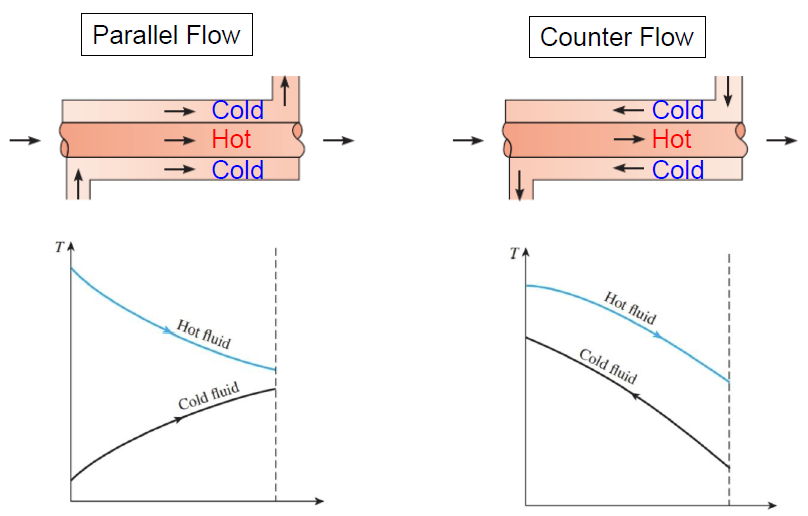
\includegraphics[width=1.0\linewidth]{images/concentric_tube_heat_exchangers.png}
    \end{figure}
    Counter-flow allows the exit temperatures of both fluids to be different.
    \item Cross-flow heat exchangers
    \begin{figure}[H]
        \centering
        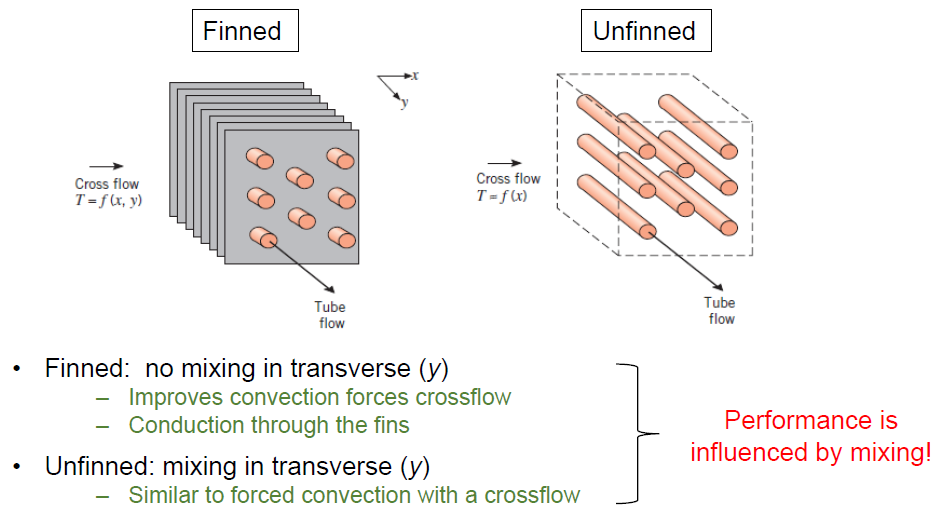
\includegraphics[width=1.0\linewidth]{images/cross_flow_heat_exchanger.png}
    \end{figure}
    \item Shell-and-Tube heat exchanger
    \begin{figure}[H]
        \centering
        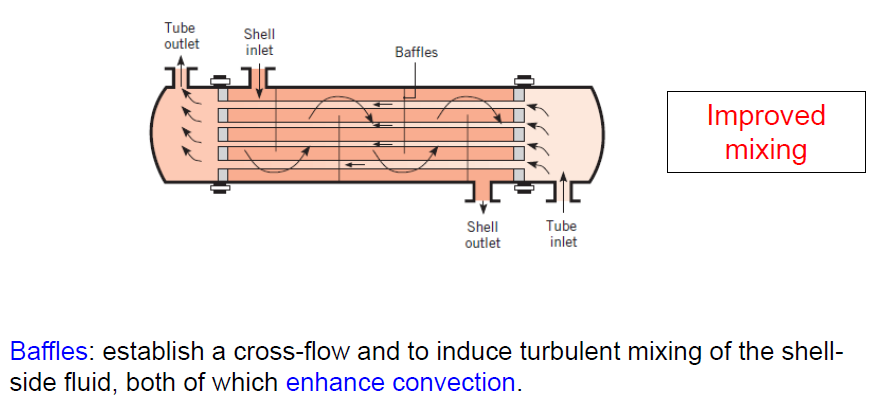
\includegraphics[width=1.0\linewidth]{images/shell_and_tube_heat_exchanger.png}
    \end{figure}
    \item Compact heat exchanger
    \begin{figure}[H]
        \centering
        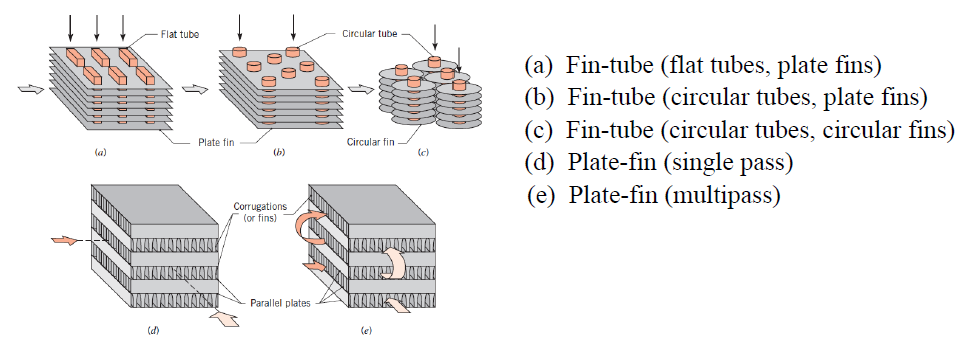
\includegraphics[width=1.0\linewidth]{images/compact_heat_exchanger.png}
    \end{figure}
\end{itemize}
\underline{ \textbf{Overall heat transfer coefficient \color{red}U\color{black}}}
\begin{itemize}
    \item heat gained in cold fluid (c) = heat lost from hot fluid (h)
    \begin{equation*}
        U = \frac{1}{\frac{1}{h_i}+\frac{1}{h_o}}
    \end{equation*}
    \begin{equation*}
        \frac{1}{UA} = \frac{1}{(UA)_c} = \frac{1}{(UA)_h}
    \end{equation*}
    \begin{align*}
        \frac{1}{UA} &= \color{red}\underbrace{\frac{1}{(\eta_O h A)_c} +\frac{1}{(\eta_O h A)_h}}_{\text{Convection}}\color{black} \\
        &+ \color{magenta}\underbrace{\frac{R_{f,c}^{''}}{(\eta_O A)_c} +\frac{R_{f,c}^{''}}{(\eta_O A)_h}}_{\text{Fouling}}\color{black} + \color{blue}\underbrace{R_w }_{\text{Conduction}} \color{black}
    \end{align*}
    \begin{itemize}
        \item $R_{f}^{''}=$ fouling factor for a unit surface area, ($m^2\cdot K/W$)
        \begin{figure}[H]
            \centering
            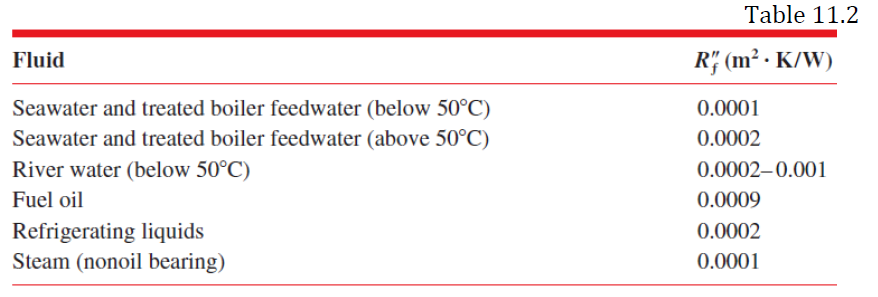
\includegraphics[width=1.0\linewidth]{images/Fouling_table.png}
        \end{figure}
        \item \color{blue} $R_w$ \color{black} = Wall conduction resistance, (K/W) 
        \item $\eta_o = $ Overall surface efficiency of fin array
    \end{itemize}
\end{itemize}
\underline{ \textbf{Methodology for Heat Exchanger Calculations}}
\begin{itemize}
    \item Log Mean Temperature Difference (\color{blue}LMTD\color{black}) Method 
    \begin{align*}
        \dot{Q} &= UA\Delta T_{lm} \\
        \Delta T_{lm} &= \frac{\Delta T_1 - \Delta T_2}{\ln(\Delta T_1 / \Delta T_2)}
    \end{align*}
    \color{red} Evaluation of $\Delta T_1$ and $\Delta T_2$ depends on the heat exchanger types.\color{black}
    \begin{itemize}
        \item Parallel-flow heat exchanger
        \begin{align*}
            \Delta T_1 &= T_{h,i} - T_{c,i} \\
            \Delta T_2 &= T_{h,o} - T_{c,o}
        \end{align*}
        \color{blue} $T_{c,o}$ cannot exceed $T_{h,o}$\color{black}
        \item Counter-flow heat exchanger
        \begin{align*}
            \Delta T_1 &= T_{h,i} - T_{c,o} \\
            \Delta T_2 &= T_{h,o} - T_{c,i}
        \end{align*}
         \color{blue} $T_{c,o}$ can exceed $T_{h,o}$\color{black}
         \item For \color{blue} equivalent values of UA \color{black} and inlet temperatures, \color{blue} $\Delta T_{lm,CF}> \Delta T_{lm,PF}$.
    \end{itemize}
    \item \underline{\textbf{Correction Factor F:}} applies to complex heat exchangers like \color{blue}shell-and-tube \color{black} and \color{blue} cross-flow heat exchangers \color{black}.
    \begin{equation*}
        \Delta T_{lm} = F \Delta T_{lm,CF}
    \end{equation*}
    $F$ measures the \color{red} deviation of $\Delta T_{lm}\;$\color{black} from the corresponding \color{red} counter-flow \color{black} case. 
    \begin{figure}[H]
        \centering
        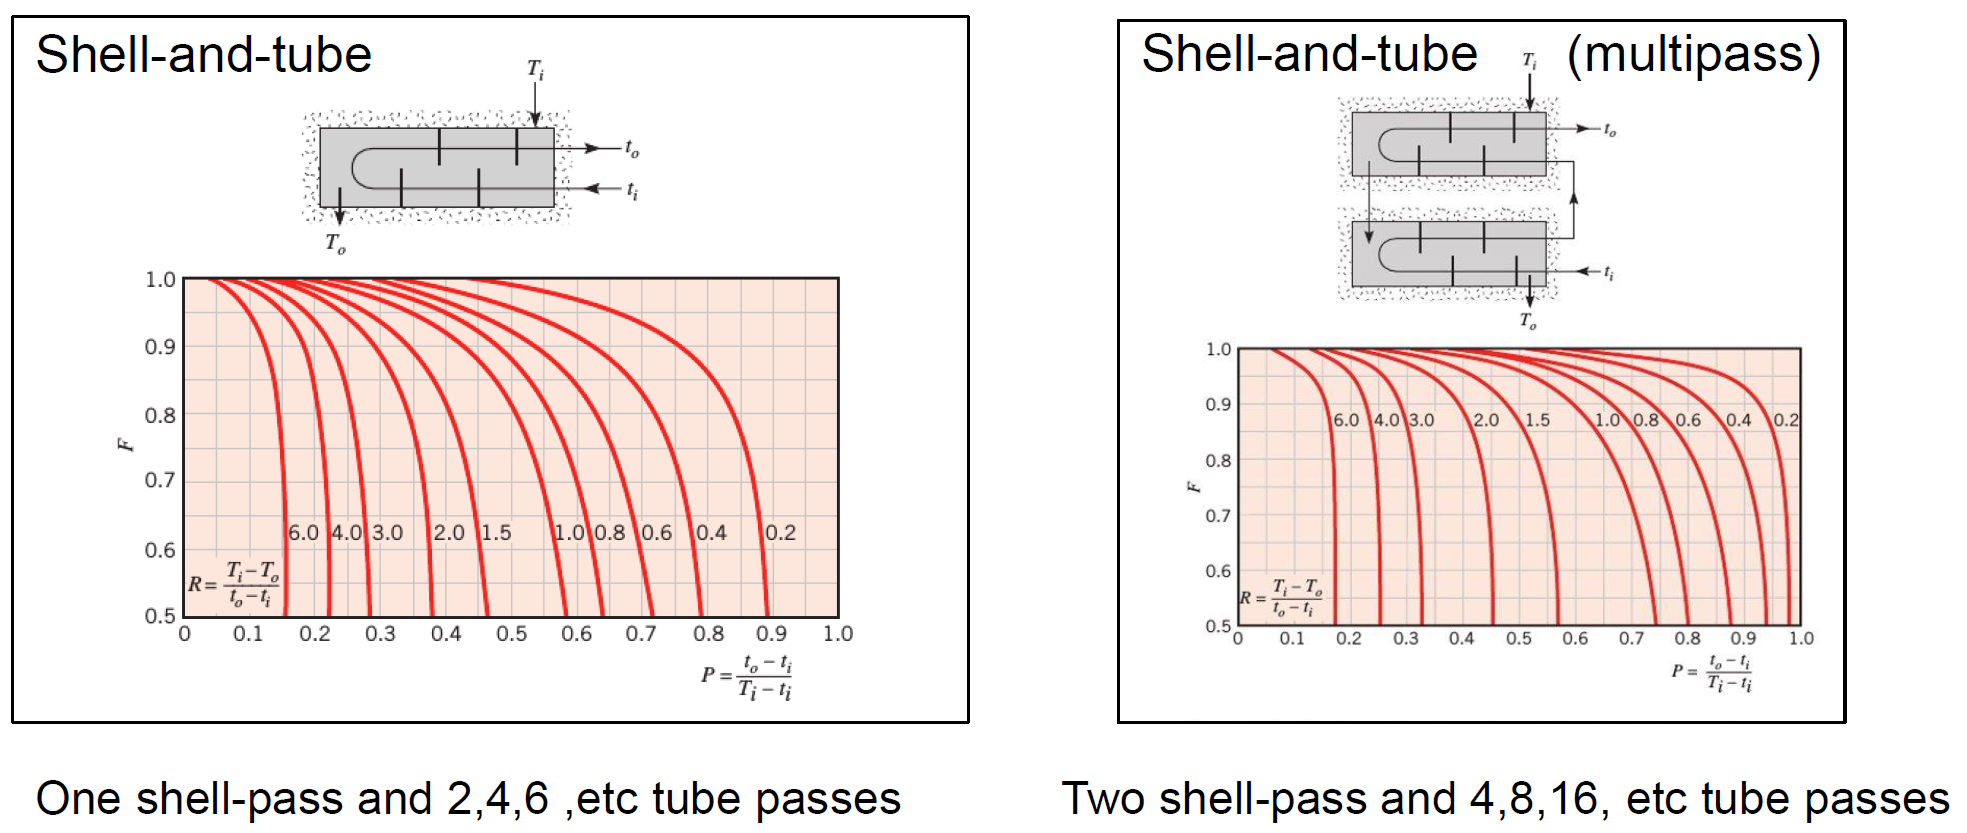
\includegraphics[width=1.0\linewidth]{images/heat_exchanger_correction_factor_1.png}
    \end{figure}
    Note that
    \begin{align*}
        \text{Uppercase} &\rightarrow \text{hot stream} \\
        \text{Lowercase} &\rightarrow \text{cold stream}
    \end{align*}
    \begin{figure}[H]
        \centering
        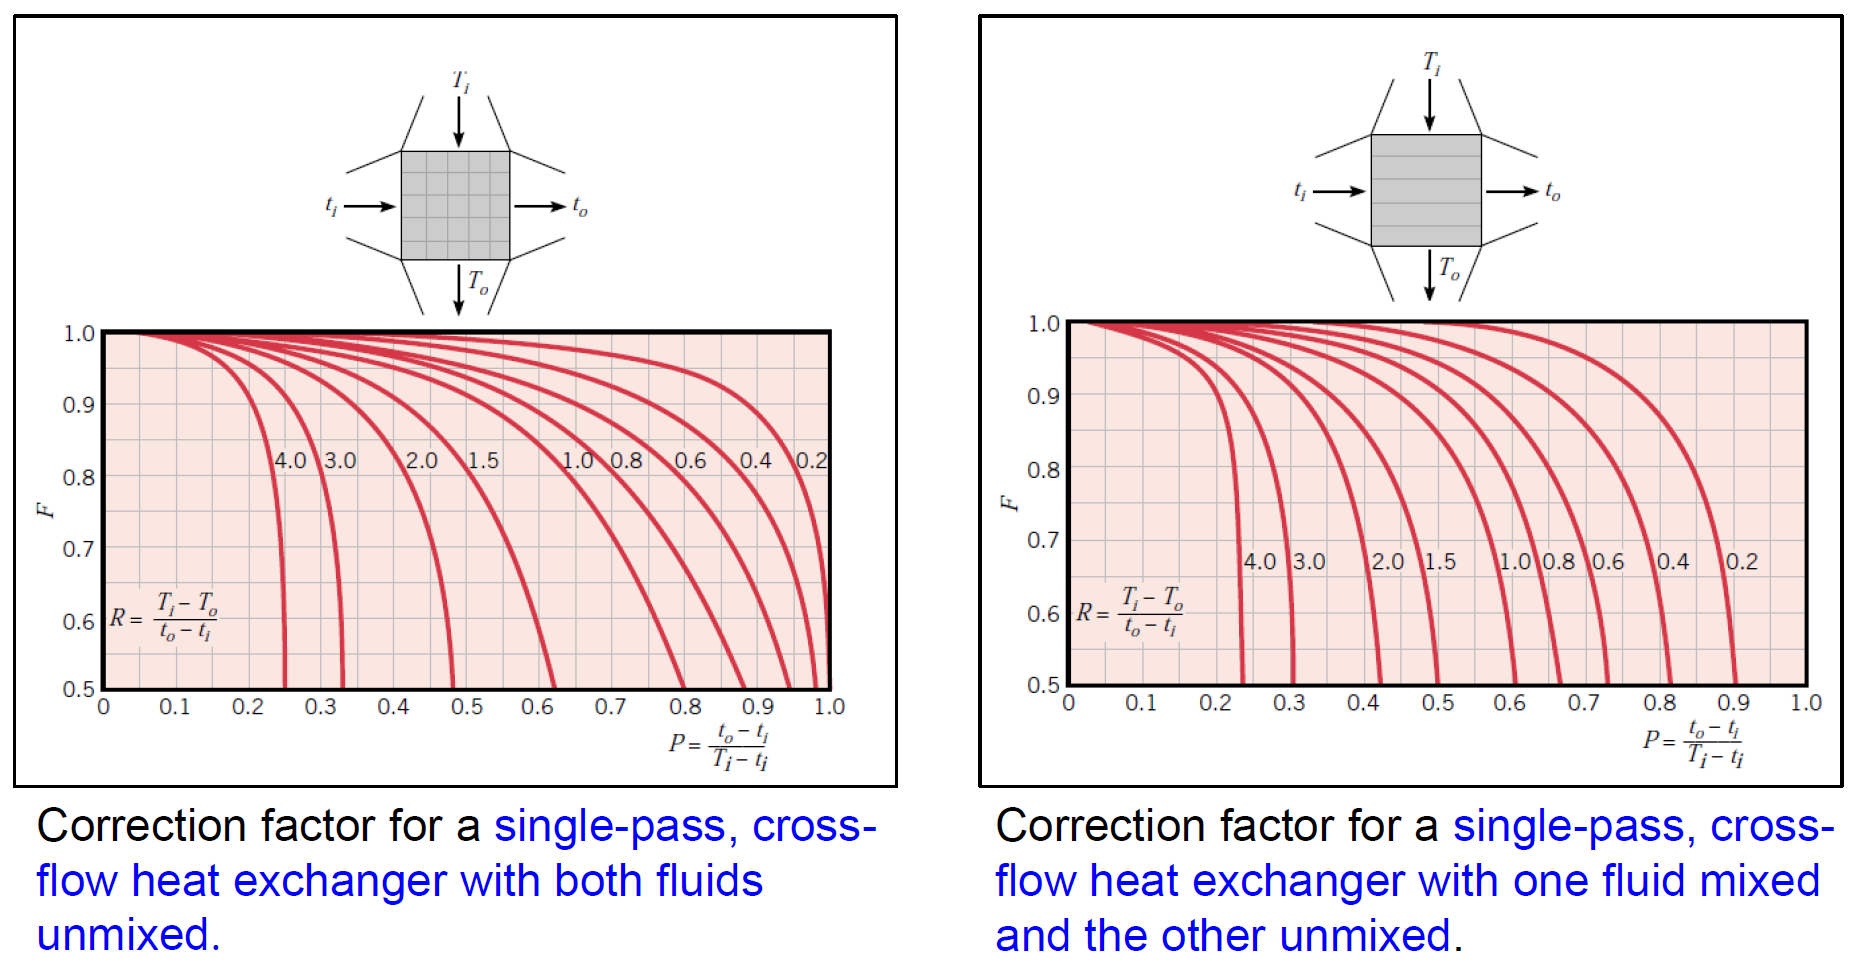
\includegraphics[width=1.0\linewidth]{images/heat_exchanger_correction_factor_2.png}
    \end{figure}
\end{itemize}


\Large \textbf{\underline{Radiation}}


\begin{itemize}
    \item \color{blue} \textbf{Emission:} \color{black} heat transfer from matter resulting in a \color{blue} reduction in its thermal energy. \color{black} 
    \item \color{blue} \textbf{Absorption:} \color{black} radiation may also be intercepted and absorbed by matter, resulting in an increase in thermal energy.
\end{itemize}

\large \textbf{\underline{Emission}}


\begin{itemize}
    \item For gas, liquid, and semitransparent solid, \color{blue} emission \color{black} is a \color{blue} volumetric \color{black} phenomenon.
    \item For opaque solid and liquid, \color{blue} emission \color{black} is a \color{blue} surface phenomenon\color{black} (emission originates from atoms and molecules within 1 $\mu m$ of the surface).
\end{itemize}
\begin{align*}
    \lambda &= \frac{c}{v} \\
    \text{where } \lambda &= \text{wavelength} \\
    v &= \text{frequency} \\
    c &= 2.998\times 10^8 \; m/s
\end{align*}

\large \textbf{\underline{Blackbody Radiation}}
\begin{itemize}
    \item Emissive power at a specific wavelength (Planck distribution)
    \begin{equation*}
        E_{\lambda,b}(\lambda,T) = \frac{C_1}{\lambda^5 [\exp(\frac{C_2}{\lambda T})-1]}
    \end{equation*}
    \begin{itemize}
        \item First radiation constant: $C_1 = 3.742\times 10^8\; W\cdot \mu m^4/m^2$
        \item Second radiation constant: $C_2 = 1.439 \times 10^4\; \mu m \cdot K$
    \end{itemize}
    \item Wien's displacement law:
    \begin{equation*}
        \lambda_{max} T = C_3 = 2898\; \mu m \cdot K
    \end{equation*}
    \item Total emissive power of a blackbody:
    \begin{align*}
        E_b &= \int_{0}^{\infty} E_{\lambda,b} d\lambda = \color{blue}\sigma T^4\color{black} \\
        \text{where } \sigma &= 5.670 \times 10^{-8} W/m^2\cdot K^4
    \end{align*}
    \item Blackbody radiation function $f_{\lambda}$
    \begin{itemize}
        \item $f_{\lambda}$ is a fraction of radiation emitted at $T$ in a fixed wavelength band.
        \item Defined as
        \begin{equation*}
            f_{\lambda}(T) = \frac{\int^{\infty}_{0}E_{\lambda,b}d\lambda }{\sigma T^4}
        \end{equation*}
        \item Use $\lambda\times T$ to find the tabulated value of $f_{\lambda}$
        \begin{figure}[H]
            \centering
            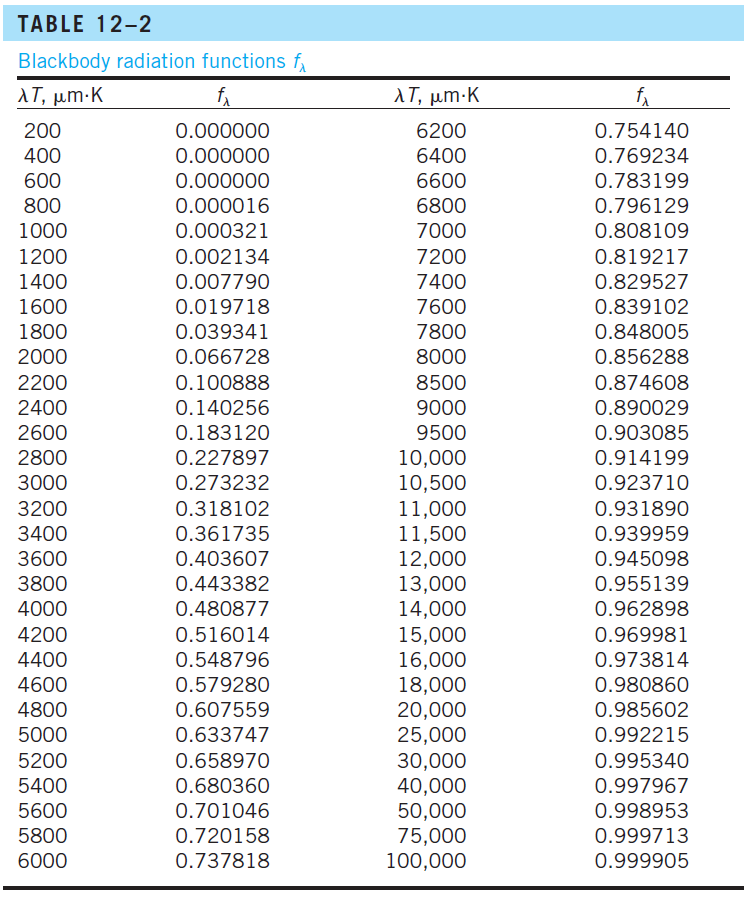
\includegraphics[width=1.0\linewidth]{images/blackbody_radiation_functions.png}
        \end{figure}
    \end{itemize}
\end{itemize}


\section{Week 5}
\large \textbf{\underline{View Factor}}

\begin{itemize}
    \item Radiation heat transfer between surfaces depends on the \color{blue} orientation of the surfaces. \color{black}
    \begin{figure}[H]
        \centering
        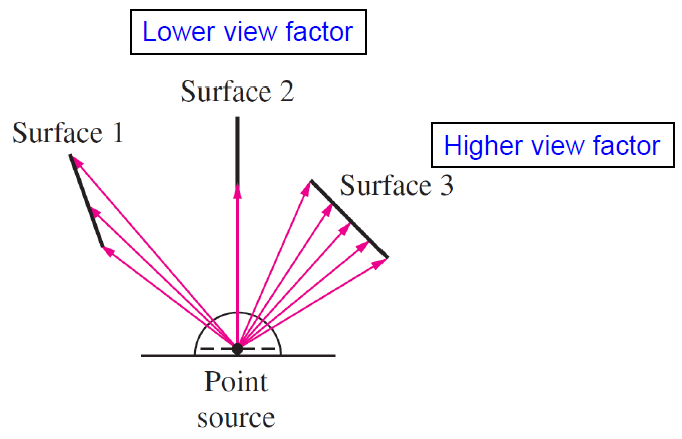
\includegraphics[width=1.0\linewidth]{images/view_factor_1.png}
    \end{figure}
    \item View factor by Table and Chart:
    \begin{figure}[H]
        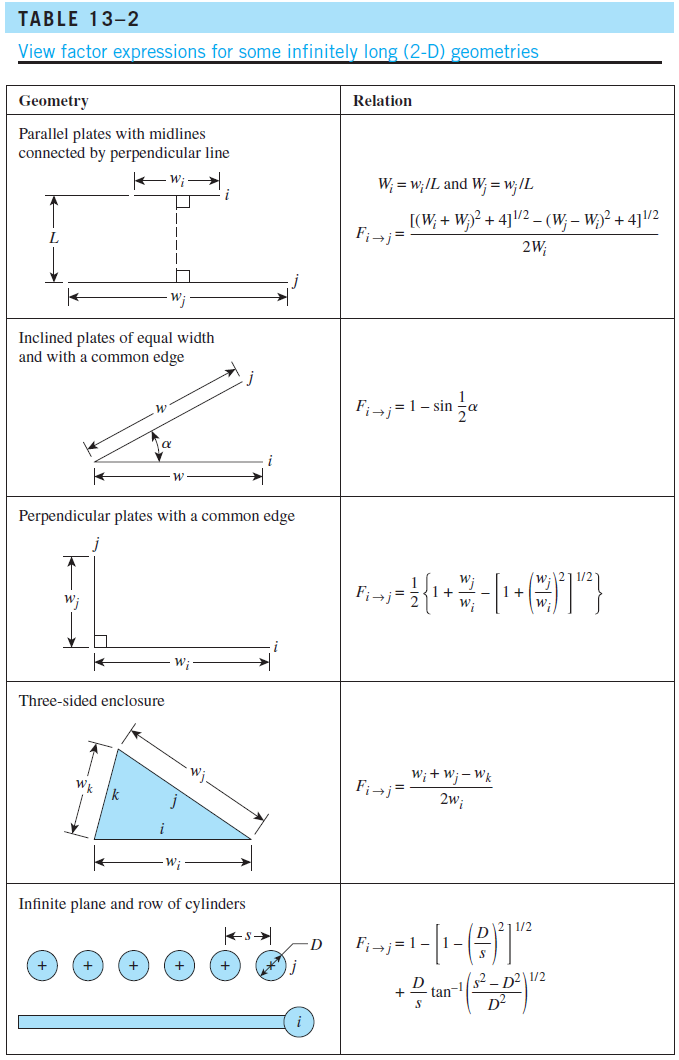
\includegraphics[width=1.0\linewidth]{images/View_factor_table_13_2.png}
    \end{figure}
    \begin{figure}[H]
        \centering
        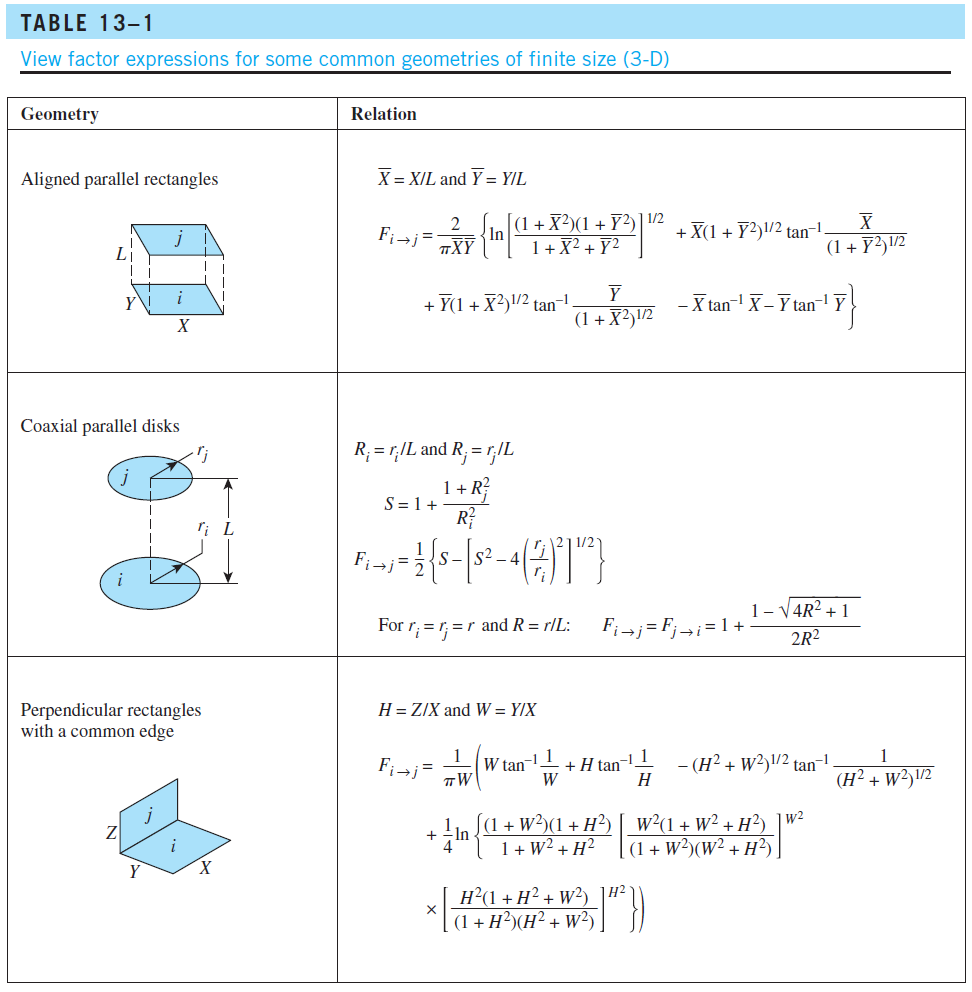
\includegraphics[width=1.0\linewidth]{images/View_factor_table_13_1.png}
    \end{figure}
    
    \begin{figure}[H]
        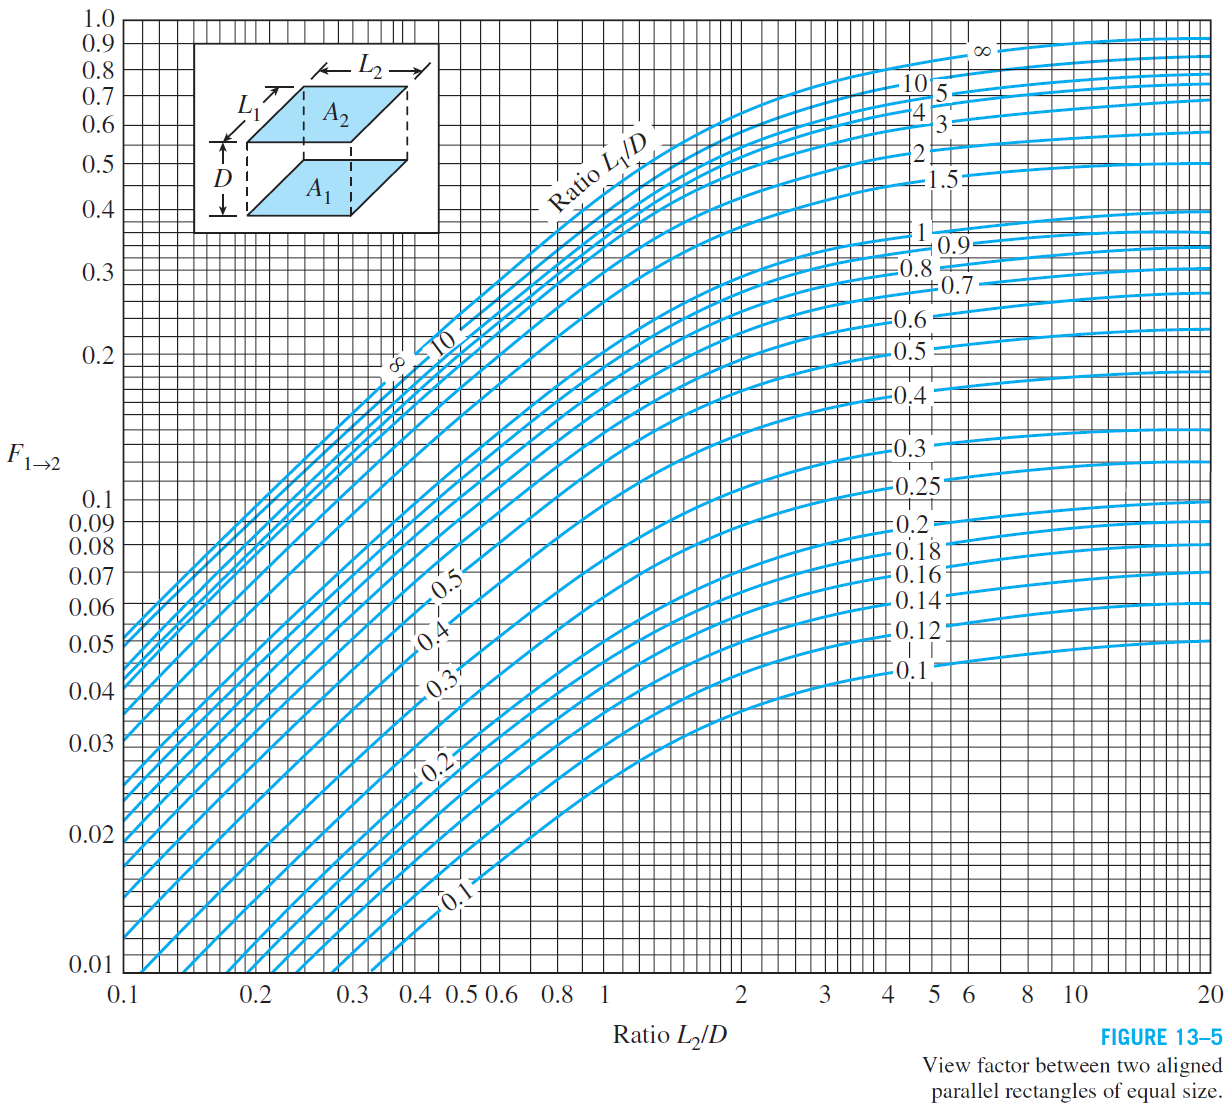
\includegraphics[width=1.0\linewidth]{images/view_factor_chart_1.png}
    \end{figure}
    \begin{figure}[H]
        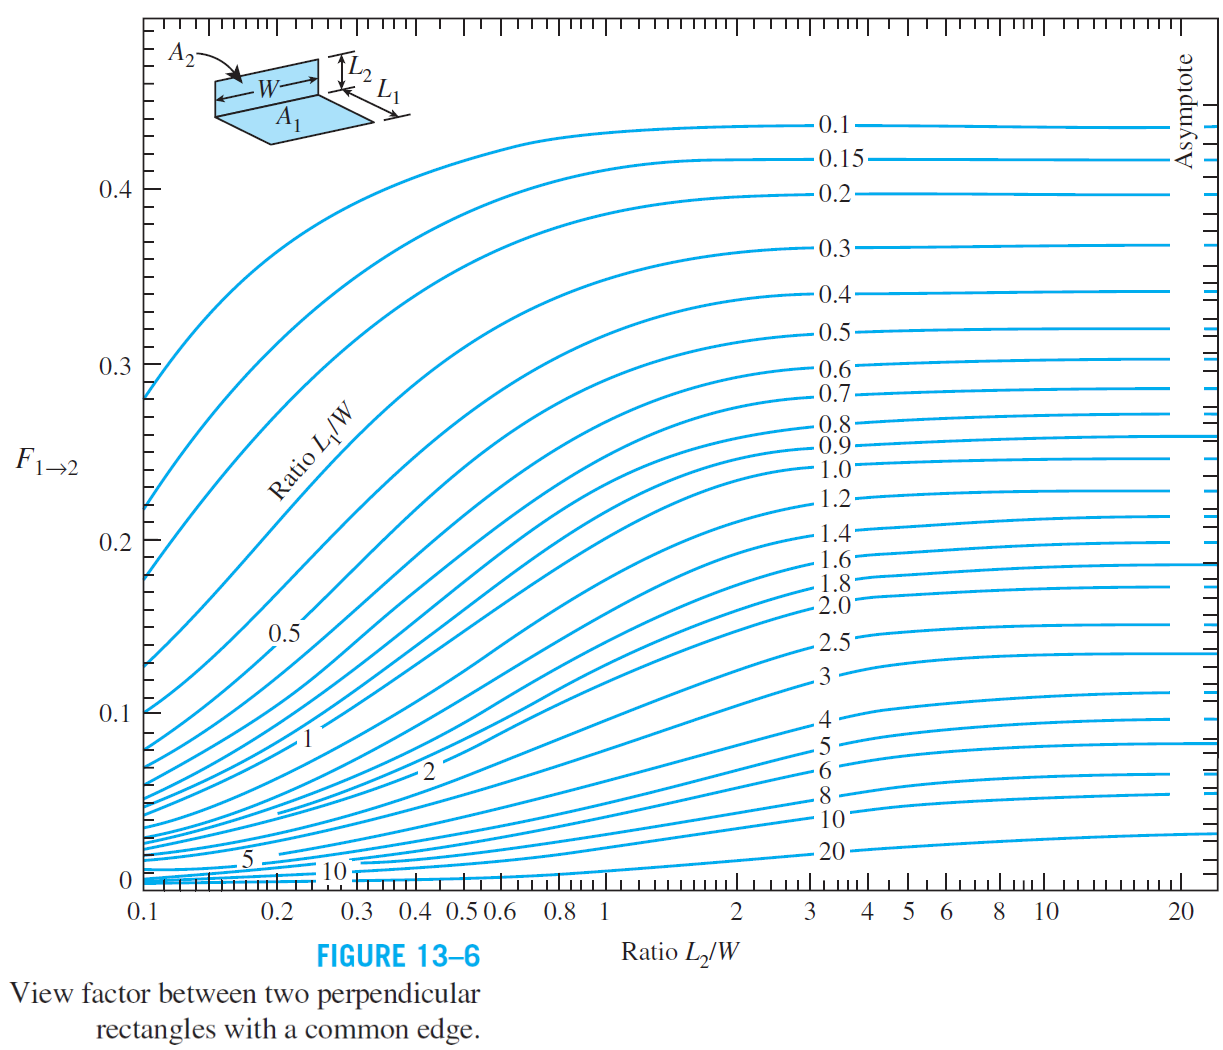
\includegraphics[width=1.0\linewidth]{images/view_factor_chart_2.png}
    \end{figure}
    \begin{figure}[H]
        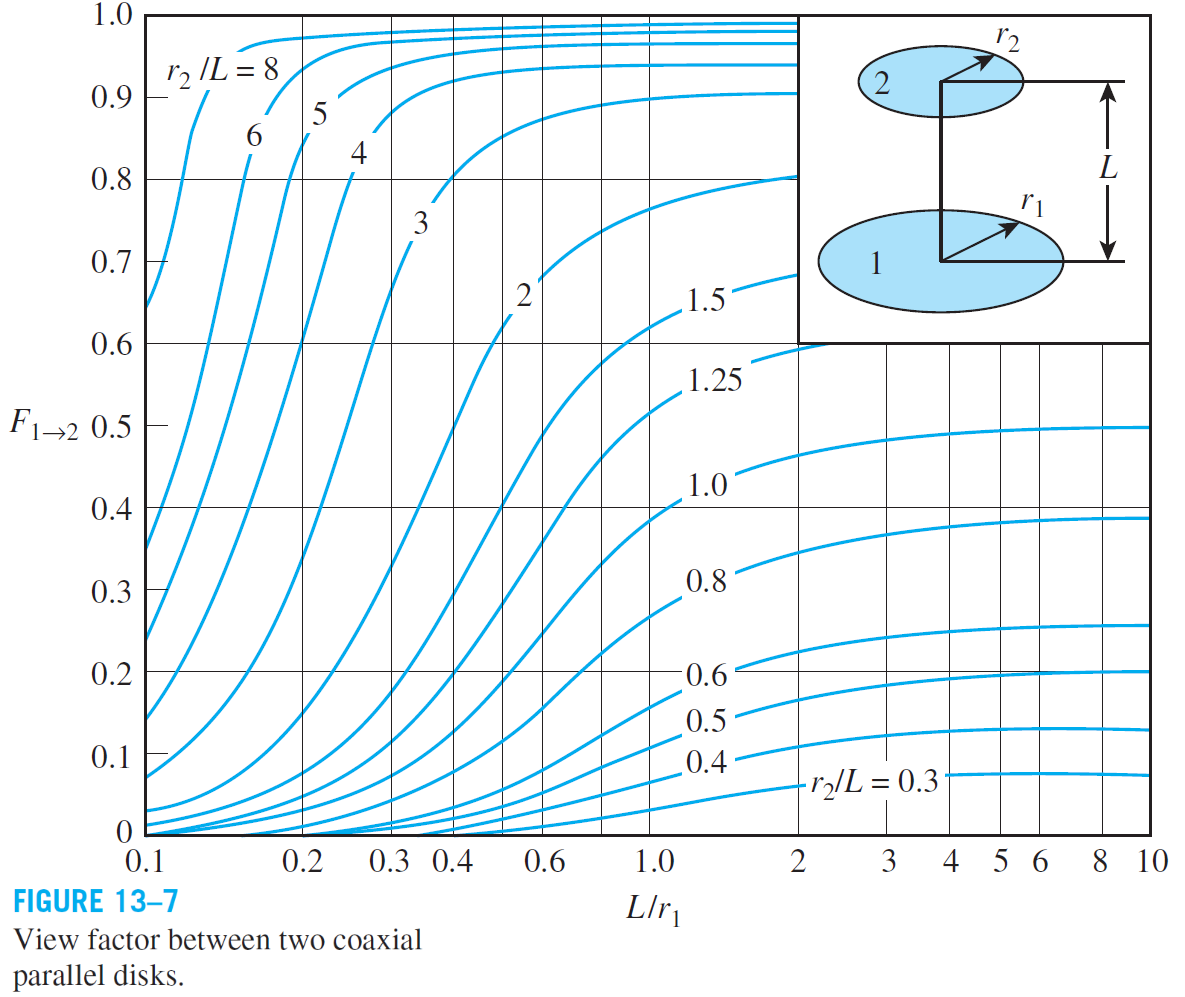
\includegraphics[width=1.0\linewidth]{images/view_factor_chart_3.png}
    \end{figure}
    \item View factor by analytical derivation
    \begin{itemize}
        \item Rule of Reciprocity
        \begin{equation*}
            A_i F_{ij} = A_j F_{ji}            
        \end{equation*}
        \item Rule of Summation (for enclosed geometry)
        \begin{equation*}
            \sum_{j=1}^{N} F_{ij} = 1
        \end{equation*}
        \item Important Geometries
        \begin{figure}[H]
            \centering
            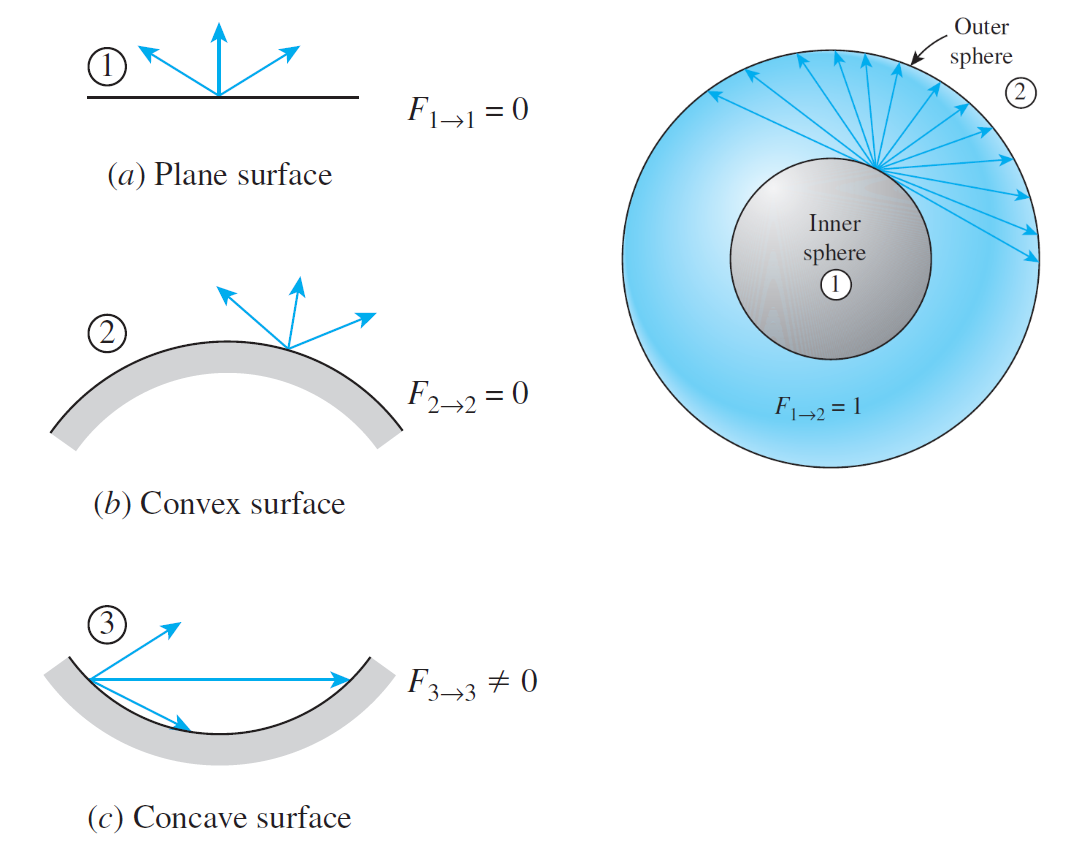
\includegraphics[width=0.9\linewidth]{images/view_factor_important_geometries.png}
        \end{figure}
    \end{itemize}
    \item Blackbody Radiation Exchanger
    \begin{itemize}
        \item Net radiative exchange
        \begin{align*}
            \dot{Q}_{ij} &= \left(\frac{\text{Radiation leaving surface i}}{\text{that strikes surface j}}\right) \\
            &- \left(\frac{\text{radiation leaving surface j}}{that strikes surface i}\right)\\
            \dot{Q}_{ij} &= \dot{Q}_{i\to j} - \dot{Q}_{j \to i}
        \end{align*}
        \item For a blackbody of Emissive Power $=E_{bi}$
        \begin{equation*}
            \dot{Q}_{ij} = A_i F_{ij} \sigma (T_i^4-T_j^4)
        \end{equation*}
        \item Net radiation transfer from surface i due to exchange with all (N) surfaces of an enclosure:
        \begin{equation*}
            \dot{Q}_i = \sum_{j=1}^{N} A_i F_{ij} \sigma (T_i^4-T_j^4) 
        \end{equation*}
    \end{itemize}
\end{itemize}
\section{Week 7}
\textbf{\underline{Pole-Zero Placement}}

When a transfer function is given,
\begin{equation*}
    G_p (z) = \frac{z-0.1}{(z-0.8)\cdot (z^2-z+0.34)} \; ,
\end{equation*}

and the question asks for a pole/zero placement that makes the system goes through a certain point that was not originally on the root locus,
\begin{equation*}
    z^* = 0.4+j\,0.17 \; ,
\end{equation*}

Do the following steps:
\begin{enumerate}
    \item Compute $G_p(z^*)$. In this example,
    \begin{align*}
        G_p(z^*) &= -1.38451 - j\, 9.3625 \\
        &= 9.46432 \, \angle -98.41^{\circ} 
    \end{align*}
    \item Obtain the angle contribution the controller needs to provide. In this case,
    \begin{align*}
        \theta &= -180^{\circ} - (-98.41^{\circ}) \\
        &= -81.58^{\circ} 
    \end{align*}
    \item Use geometry to determine the pole/zero location (not sure if there's a better and quicker way).
\end{enumerate}
\begin{figure}[h]
    \centering
    \includegraphics[width=1.0\linewidth]{images/pole_placement.png}
\end{figure}
    
\textbf{\large Cancellations:}
\begin{itemize}
    \item Cancellation of unstable poles of $G_p$ at the implementation stage leads to instability, because the value of physical poles cannot be precisely measured.
    \item Cancellation taken place at the computational plane is harmless.
    \item Cancel a pole with real parts greater than 0 in z-domain is more worrisome than cancelling a pole with negative real part.
    \begin{equation*}
        \begin{cases}
            \frac{4(z+0.5)}{(z+0.5)(z-0.1)} \\
            y(k) = C_1 (-0.5)^k + C_2 (0.1)^k
        \end{cases}
    \end{equation*}
    Ex. $(z-0.1)$ is the more worrying pole because $C_2 (0.1)^k$ is growing while $C_1 (-0.5)^k$ is neutral and ringing.
\end{itemize}

\section{Week 8}
\Large \textbf{{\color{red}\underline{Normal Shocks}}}

\begin{itemize}
    \item Non-isentropic process
    \item Non-trivial solution for {\color{blue}compressible} flows:
    \begin{itemize}
        \item Density ratio:
        \begin{equation*}
            \frac{\rho_2}{\rho_1} = \frac{u_1}{u_2} = \frac{(\gamma + 1)M_1^2}{2+(\gamma - 1)M_1^2}
        \end{equation*}
        \item Pressure ratio:
        \begin{equation*}
            \frac{P_2}{P_1} = 1 + \frac{2 \gamma}{\gamma + 1} (M_1^2 - 1)
        \end{equation*}
        \item Temperature ratio:
        \begin{align*}
            \frac{T_2}{T_1} &= \left[ 1 + \frac{2\gamma}{\gamma + 1}(M_1^2 - 1) \right]\\
            &\cdot \frac{2+(\gamma - 1)M_1^2}{(\gamma + 1)M_1^2}
        \end{align*}
        \item Mach number ratio:
        \begin{equation*}
            M_2^2 = \frac{1+\frac{\gamma - 1}{2}M_1^2}{\gamma M_1^2 - \frac{\gamma - 1}{2}}
        \end{equation*}
        \item Entropy $s$ ratio
        \begin{align*}
            s_2 - s_1 &= c_p \ln\left(\left[1+\frac{2\gamma(M_1^2 - 1)}{\gamma+1}\right]\right. \\
            &\cdot \left. \frac{2+(\gamma-1)M_1^2}{(\gamma + 1)M_1^2}\right) \\
            &- R \ln\left( 1 + \frac{2\gamma}{\gamma + 1}(M_1^2 - 1) \right)
        \end{align*}
        Note that since $s_2 - s_1 \geq 0$, $\therefore M_1^2\geq 1$. Thus normal shock only occurs for supersonic flow.
    \end{itemize}
\end{itemize}

\large \textbf{\underline{Stagnation properties cross a normal shock}}

\begin{itemize}
    \item Non-isentropic processes across the shock:
    \begin{itemize}
        \item {\color{blue}Stagnation Pressure Change}
        \begin{equation*}
            \frac{P_{0,2}}{P_{0,1}} = e^{-\frac{(s_2-s_1)}{R}} \leq 1
        \end{equation*}
        \item {\color{blue}Stagnation Temperature} is constant across the normal shock
        \begin{equation*}
            T_{0,1} = T_{0,2}
        \end{equation*}
    \end{itemize}
\end{itemize}

\Large \textbf{{\color{red}\underline{Oblique Shocks}}}

Def: oblique shocks are waves occurred at concave corners. It is a {\color{red}non-isentropic} process.
\begin{figure}[H]
    \centering
    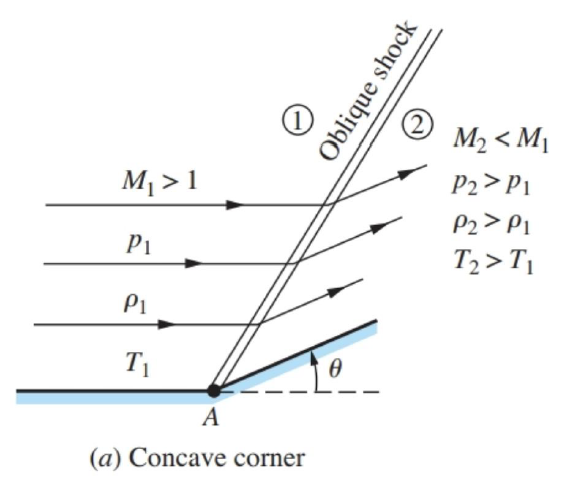
\includegraphics[width=1.0\linewidth]{images/oblique_shock_concave.png}
\end{figure}

Freebody Diagram:

\begin{figure}[H]
    \centering
    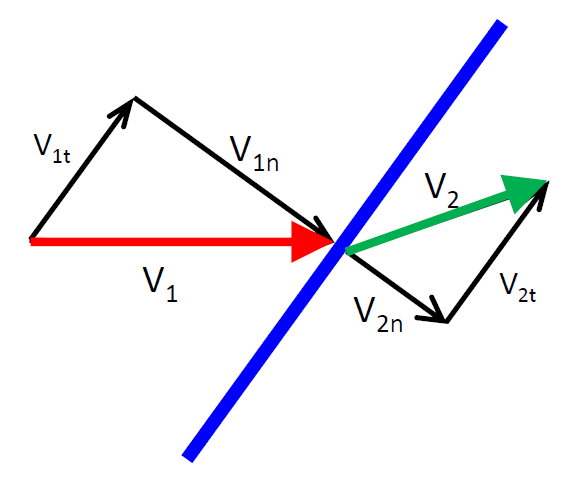
\includegraphics[width=1.0\linewidth]{images/oblique_shocks.png}
\end{figure}
\begin{itemize}
    \item Tangential component unchanged, $V_{1t} = V_{2t}$
    \item Normal component reduces, $V_{2n}<V_{1n}$
\end{itemize}

\textbf{{\color{blue}\underline{A Wedge Case}}}
\begin{itemize}
    \item {\color{red}Upstream of the shock:}
    \begin{figure}[H]
        \centering
        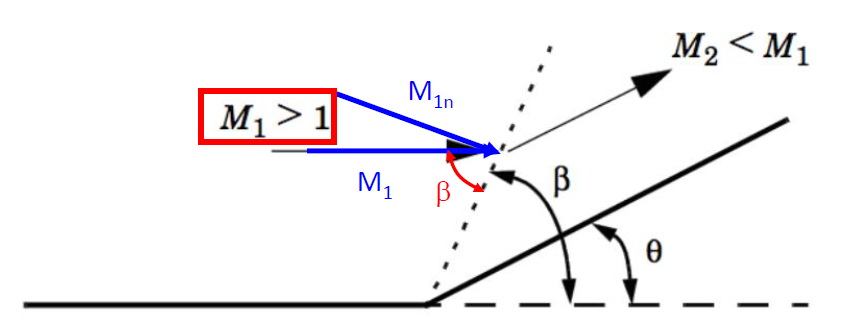
\includegraphics[width=1.0\linewidth]{images/oblique_shocks_upstream.png}
    \end{figure}
    \begin{equation*}
        M_1 = \frac{M_{1n}}{\sin(\beta)}
    \end{equation*}
    Since for a shock to form, it is required that $M_{1n}>1$. Thus, {\color{blue}$M_1 > 1$}. 
    
    \item {\color{red}Downstream of the shock:}
    \begin{figure}[H]
        \centering
        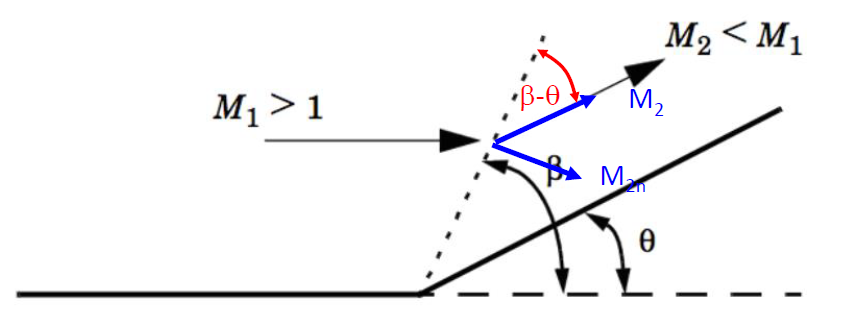
\includegraphics[width=1.0\linewidth]{images/oblique_shocks_downstream.png}
    \end{figure}
    \begin{equation*}
        M_2 = \frac{M_{2n}}{\sin(\beta - \theta)}
    \end{equation*}
    Flow after the shock must be subsonic, $M_{2n}<1$. However, {\color{blue}$M_2$ not necessarily $< 1$}.
    \item Ratios:
    \begin{itemize}
        \item Mach number ratio
        \begin{equation*}
            M_{n,2}^2 = \frac{1+[(\gamma - 1)/2]M_{n,1}^2}{\gamma M_{n,1}^2-(\gamma - 1)/2}
        \end{equation*}
        \item Density ratio
        \begin{equation*}
            \frac{\rho_2}{\rho_1} = \frac{(\gamma+1)M_{n,1}^2}{2+(\gamma-1)M_{n,1}^2}
        \end{equation*}
        \item Pressure ratio
        \begin{equation*}
            \frac{P_2}{P_1} = 1+ \frac{2\gamma}{\gamma + 1}(M_{n,1}^2 - 1)
        \end{equation*}
        \item Temperature ratio
        \begin{equation*}
            \frac{T_2}{T_1} = \frac{P_2}{P_1} \cdot \frac{\rho_1}{\rho_2}
        \end{equation*}
        \item Relation between $\theta$, $\beta$, $M$
        \begin{figure}[H]
            \centering
            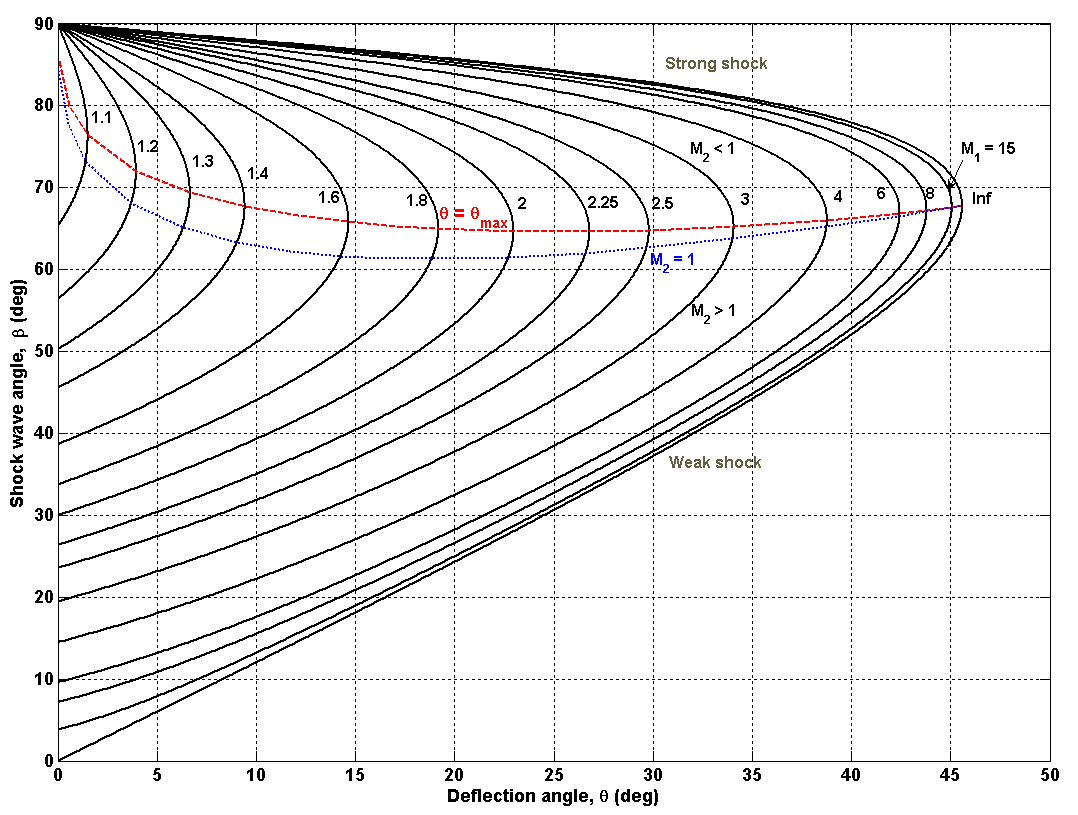
\includegraphics[width=1.0\linewidth]{images/angle-mach-relation.png}
        \end{figure}
        \begin{equation*}
            \tan(\theta) = 2\cot(\beta)\frac{\left(M_1^2\sin^2(\beta)\right)-1}{M_1^2 \left(\gamma + \cos(2\beta)\right)+2}
        \end{equation*}
        \item When $\theta = 0 ^{\circ}$, then $\beta = 90 ^{\circ} \rightarrow$ the normal shock solution.
        \item For every $\theta$ there are two solutions for $\beta$: the \textbf{weak shock} (smaller value of $\beta$) and the \textbf{strong shock} (larger value of $\beta$) - {\color{blue}the weak shock almost always prevails.}
        \begin{figure}[H]
            \centering
            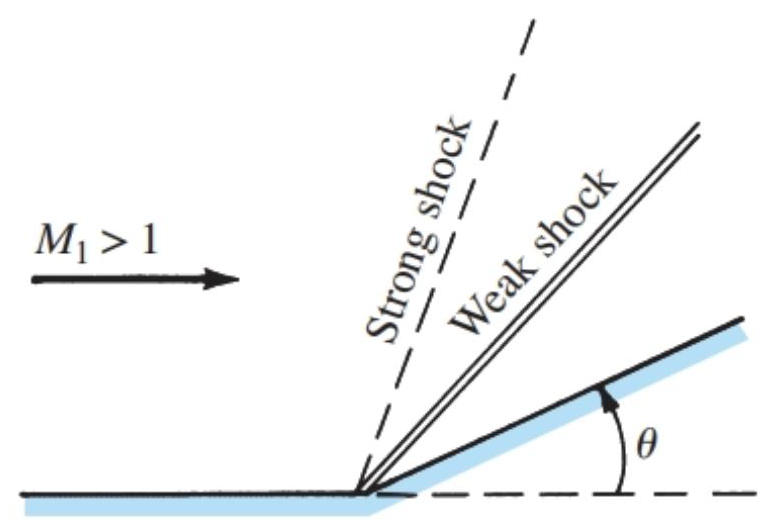
\includegraphics[width=0.8\linewidth]{images/weak_shock.png}
        \end{figure}
    \end{itemize}
\end{itemize}

\textbf{{\color{blue}\underline{Expansion Waves}}}

Def: expansion waves occurred at convex corners. It is a {\color{red}isentropic} process.
\begin{figure}[H]
    \centering
    \includegraphics[width=1.0\linewidth]{images/expansion_wave_convex.png}
\end{figure}

\textbf{\large {\color{red}\underline{Expansion Fan}}}

\begin{itemize}
    \item The flow through the expansion fan is {\color{blue}ISENTROPIC} (thus, $T_{0,2}=T_{0,1}$ and $P_{0,2}=P_{0,1}$)
    \item Prandtl-Meyer Function (function of the incoming Mach number)
    \begin{align*}
        v(M) &= \sqrt{\frac{\gamma+1}{\gamma-1}}\tan^{-1}\left(\sqrt{\frac{\gamma-1}{\gamma+1}(M^2-1)}\right) \\
        &- \tan^{-1}\left(\sqrt{M^2-1}\right)
    \end{align*}
    \item Upstream-Downstream relation:
    \begin{equation*}
        \theta = v(M_2) - v(M_1)
    \end{equation*}
    \begin{figure}[H]
        \centering
        \includegraphics[width=1.0\linewidth]{images/expansion_wave_up_downstream.png}
    \end{figure}
    \begin{itemize}
        \item Mach angles $\alpha_1$ and $\alpha_2$ (also written as $\mu_1$ and $\mu_2$)
        \begin{align*}
            \alpha_1 = \mu_1 &= \sin^{-1}\left(\frac{1}{M_1}\right) \\
            \alpha_2 = \mu_2 &= \sin^{-1}\left(\frac{1}{M_2}\right)
        \end{align*}
    \end{itemize}
    \item Ratios (use isentropic relations)
    \begin{itemize}
        \item Stagnation pressure $P_0$ is {\color{blue}unchanged}
        \item Pressure ratio:
        \begin{equation*}
            \frac{P_2}{P_1} = \left(\frac{1+\frac{\gamma-1}{2}M_1^2}{1+\frac{\gamma-1}{2}M_2^2}\right)^{\frac{\gamma}{\gamma-1}} = 0.6
        \end{equation*}
        \item Temperature ratio:
        \begin{equation*}
            \frac{T_2}{T_1} = \left(\frac{1+\frac{\gamma-1}{2}M_1^2}{1+\frac{\gamma-1}{2}M_2^2}\right)= 0.86
        \end{equation*}
        \item Density ratio:
        \begin{equation*}
            \frac{\rho_2}{\rho_1} = \left(\frac{1+\frac{\gamma-1}{2}M_1^2}{1+\frac{\gamma-1}{2}M_2^2}\right)^{\frac{1}{\gamma-1}}= 0.69
        \end{equation*}
    \end{itemize}
\end{itemize}

\large \textbf{\underline{{\color{red}Pitot-Static Tubes}}}
\begin{figure}[H]
    \centering
    \includegraphics[width=1.0\linewidth]{images/Pitot_static_tubes.png}
\end{figure}

\large \textbf{\underline{{\color{red}Lift and Drag}}}
\begin{figure}[H]
    \centering
    \includegraphics[width=1.0\linewidth]{images/Compressible_Aerodynamics.png}
\end{figure}

\begin{align*}
    R &= (p_3 - p_2 ) \cdot c \\
    L &= (p_3 - p_2 ) \cdot c \cdot \cos(\alpha) \\
    D &= (p_3 - p_2 ) \cdot c \cdot \sin(\alpha)
\end{align*}

\begin{itemize}
    \item Coefficient of Lift:
    \begin{align*}
        c_l &= \frac{L}{\frac{1}{2}\gamma P_1 M_1^2 S} \\
        \text{where } S &= c \times 1
    \end{align*}
    Note that S = chord length $\times$ unit depth. For 2D case, the depth is unity.
    \item Coefficient of Drag:
    \begin{equation*}
        c_d = \frac{D}{\frac{1}{2}\gamma P_1 M_1^2 S}
    \end{equation*}
\end{itemize}
\section{Week 9}
\Large \textbf{{\color{red}\underline{Mixure}}}

\begin{enumerate}
    \item Compressibility factor
    \begin{itemize}
        \item Ideal gas: 
        \begin{equation*}
            Pv = RT
        \end{equation*}
        Assumptions made:
        \begin{itemize}
            \item particles of zero size/volume
            \item no attractive forces
            \item perfectly elastic collisions
        \end{itemize}
        \item 'Compressed' ideal gas:
        \begin{align*}
            Pv &= {\color{blue}Z}RT\\
            \text{where } {\color{blue}Z} &= \frac{v_{actual}}{v_{ideal}}, \\
            {\color{blue}Z} &= \begin{cases} 
            >1, \\
            =1, \\
            < 1
            \end{cases}
        \end{align*}
    \end{itemize}
    \item {\color{blue}Reduced Pressure $P_r$}:
    \begin{equation*}
        P_r = \frac{P}{P_{cr}}
    \end{equation*}
    \item {\color{blue}Reduced Pressure $T_r$}:
    \begin{equation*}
        T_r = \frac{T}{T_{cr}}
    \end{equation*}
\end{enumerate}


\section{Week 10}
\begin{center}
    \textbf{\Large \underline{Observers}}
\end{center}
The following exemplar system will be used in the upcoming notes.
\begin{align*}
    \text{continuous} &\begin{cases}
        \dot{x}(t) = A x(t) + B u(t) \\
        y(t) = C x(t) 
    \end{cases} \\
    \text{discrete} &\begin{cases}
        x(k+1) = G x(k) + H u(k) \\
        y(k) = C x(k)
    \end{cases} \\
    T &= \text{sampling time}
\end{align*}
\textbf{\large \underline{Prediction Observers}}
\begin{itemize}
    \item State feedback controller:
    \begin{align*}
        u(k)&=-Kx \\
        \textbf{CE:} \; \; \left|zI-(G-HK)\right|\cdot X(z)&=0
    \end{align*}
    \item Estimator Equations:
    \begin{align*}  
        &\begin{cases}
            \hat{x}(k+1) = G \hat{x}(k)+H u(k) \\
            \hat{y}(k) = C \hat{x}(k)
        \end{cases} \\
        &\begin{cases}
            \Tilde{x}(k) = x(k) - \hat{x}(k) \\
            \Tilde{y}(k) = y(k) - \hat{y}(k) = C \Tilde{x}(k)
        \end{cases}
    \end{align*}
    \item Error Dynamics:
    \begin{align*}
        e(k) &= \Tilde{x}(k) \\
        e(k+1) &= G e(k) - L[ \Tilde{y}(k)] \\
        &= Ge(k)-L[C\Tilde{x}(k)] \\
        &= [G-LC]e(k) 
    \end{align*}
    \item Characteristic Equation of Error Dynamics:
    \begin{align*}
        \textbf{CE:}\;\; \left|zI-(G-LC)\right|\cdot E(z)&=0
    \end{align*}
    \begin{itemize}
        \item \textbf{Remark:} note that
        \begin{align*}
            (G-LC) &= (G-LC)^{T} \\
            &= G^T - C^T L^T
        \end{align*}
        The above relation is important when using the MATLAB 'acker()' or 'place()' command.
    \end{itemize}
    \item \textbf{Example 1.1:} The state feedback controller is designed to satisfy the continuous time CE $(s+10)^2=0$. Find gain matrix $K$.
\begin{lstlisting}
% root of feedback controller CE
s_fb = -10;
poles = [exp(s_c*T), exp(s_c*T)];
% place(A,B,poles) does not accept repeated roots
% so we use acker() here
K = acker(G,H,poles)
\end{lstlisting}
    \item \textbf{Example 1.2:} The speed of response of the observer must be 5 times faster than that of the feedback controller. Find gain matrix $L$.
\begin{lstlisting}
s_fb = -10;
s_ob = 5 * s_fb;
poles = [exp(s_ob*T), exp(s_ob*T)];
% Recall the remark on transpose made above!
L = acker(G', C', poles)'
\end{lstlisting}
\end{itemize}


\textbf{\large \underline{Current Observers}}
\begin{itemize}
    \item Error Dynamics:
    \begin{align*}
        e(k+1) &= G e(k) - L\color{red} [\Tilde{y}(k+1)] \\
        &= Ge(k)-L\color{red}[C\Tilde{x}(k+1)] \\
        &= Ge(k)-LC[ \underbrace{Gx(k)+\cancel{Hu(k)}}_{x(k+1)}-\underbrace{G\hat{x}(k)-\cancel{Hu(k)}}_{\hat{x}(k+1)}]\\
        &= Ge(k)-LCG\Tilde{x}(k) \\
        &= Ge(k)-LCGe(k) \\
        &= [G-LCG]e(k)
    \end{align*}
    \item Characteristic Equation of Error Dynamics:
    \begin{align*}
        \textbf{CE:}\;\; \left|zI-(G-LCG)\right|\cdot E(z)&=0
    \end{align*}
    \item \textbf{Remark:} note that
    \begin{align*}
        (G-LCG) &= (G-LCG)^T \\
        &= G^T - G^T C^T L^T
    \end{align*}
    \item \textbf{Example 1.3:} The speed of response of the observer must be 5 times faster than that of the feedback controller. Find gain matrix $L$.
\begin{lstlisting}
% Recall the remark on transpose made above!
L = acker(G', G'*C', poles)'
\end{lstlisting}
\end{itemize}


\printbibliography


\end{document}